\documentclass[11pt,a4paper]{article}

% Essential packages
\usepackage[utf8]{inputenc}
\usepackage[T1]{fontenc}
\usepackage{lmodern}
\usepackage[english]{babel}

% Mathematics packages
\usepackage{amsmath}
\usepackage{amssymb}
\usepackage{amsthm}
\usepackage{mathtools}
\usepackage{bm}

% Graphics and figures
\usepackage{graphicx}
\usepackage{subcaption}
\usepackage{float}
\usepackage{tikz}
\usepackage{pgfplots}
\pgfplotsset{compat=1.17}

% Algorithms
\usepackage[ruled,vlined]{algorithm2e}
\usepackage{algorithmic}

% Tables and formatting
\usepackage{booktabs}
\usepackage{array}
\usepackage{multirow}
\usepackage{longtable}

% References and citations
\usepackage{cite}
\usepackage{url}
\usepackage[colorlinks=true,citecolor=blue,urlcolor=blue,linkcolor=blue]{hyperref}

% Page layout
\usepackage[margin=2.5cm]{geometry}
\usepackage{setspace}
\usepackage{parskip}

% Additional formatting
\usepackage{enumerate}
\usepackage{enumitem}
\usepackage{xcolor}
\usepackage{caption}

% Mathematical theorem environments
\newtheorem{theorem}{Theorem}[section]
\newtheorem{lemma}[theorem]{Lemma}
\newtheorem{corollary}[theorem]{Corollary}
\newtheorem{proposition}[theorem]{Proposition}
\newtheorem{definition}[theorem]{Definition}
\newtheorem{example}[theorem]{Example}
\newtheorem{remark}[theorem]{Remark}

% Proof environment
\renewcommand{\proofname}{\textbf{Proof}}

% Custom commands for mathematical notation
\newcommand{\Real}{\mathbb{R}}
\newcommand{\Complex}{\mathbb{C}}
\newcommand{\Natural}{\mathbb{N}}
\newcommand{\Integer}{\mathbb{Z}}
\newcommand{\Prob}{\mathbb{P}}
\newcommand{\Expect}{\mathbb{E}}
\newcommand{\Variance}{\text{Var}}
\newcommand{\Cov}{\text{Cov}}
\newcommand{\norm}[1]{\left\|#1\right\|}
\newcommand{\abs}[1]{\left|#1\right|}
\newcommand{\inner}[2]{\left\langle #1, #2 \right\rangle}

% Title and author information
\title{\textbf{On the Thermodynamic Consequences of Formal Verification in Metacognitive Bayesian Information Processing: A Framework for Meta-Information Extraction with Mathematical Guarantees}}

\author{
Kundai Farai Sachikonye
}

\date{\today}

% Document begins
\begin{document}

% Title page
\maketitle

\begin{abstract}
Presented here is a metacognitive Bayesian computer vision framework that employs formal mathematical verification instead of statistical inference for visual information processing. The system integrates six mathematical components: proof-validated compression analysis using theorem provers, gas molecular dynamics modeling with Hamilton's equations, S-entropy coordinate transformation for semantic space navigation, constrained stochastic sampling with semantic gravity fields, Bayesian inference on weighted sample collections, and meta-information extraction for structural pattern identification. Unlike conventional approaches that treat ambiguity as computational noise, the framework utilizes ambiguous information as a computational resource through formal verification of multiple valid interpretations. The system operates through definite observer boundaries implemented via coordinate system constraints, ensuring mathematically well-defined measurement processes. Information elements are modeled as thermodynamic gas molecules evolving toward equilibrium states, then transformed into four-dimensional semantic coordinates where meaning relationships manifest as geometric properties. Constrained sampling employs "pogo stick jumps" with step sizes inversely proportional to local semantic gravity strength, generating samples processed through variational Bayesian inference to extract semantic clusters with quantified uncertainty bounds. Meta-information analysis identifies structural patterns enabling exponential complexity reduction through compression potential estimation. Experimental validation demonstrates $94\%$ correlation with clinical assessments across multiple imaging modalities while maintaining mathematical rigor through machine-checked proof verification of all processing stages. 
\end{abstract}

\tableofcontents

\section{Introduction}

The computational processing of visual information has traditionally operated under the assumption that information extraction and pattern recognition constitute sufficient objectives for machine vision systems \cite{szelisky2010computer, forsyth2011computer}. Contemporary approaches in computer vision, while achieving remarkable performance in classification and detection tasks \cite{krizhevsky2012imagenet, he2016deep}, fundamentally lack formal mathematical guarantees regarding the validity of their extracted representations and operate without consideration of observer effects inherent in measurement processes \cite{von2018mathematical}.

This work introduces a metacognitive Bayesian computer vision framework that diverges from conventional approaches in three fundamental aspects. Firstly, unlike traditional systems that rely on statistical inference for pattern validation \cite{bishop2006pattern, murphy2012machine}, our framework employs formal proof systems (Lean \cite{moura2015lean} and Coq \cite{bertot2013interactive}) to mathematically verify each step of the information compression and ambiguity detection process. This represents a paradigmatic shift from probabilistic validation to mathematical certainty in computer vision processing.

Secondly, where existing information-theoretic approaches in computer vision focus on minimizing entropy or maximizing information content \cite{cover2006elements, mackay2003information}, our framework specifically identifies and utilizes ambiguous information—data elements possessing multiple valid interpretations—as a computational resource rather than a source of uncertainty to be eliminated. This ambiguity-centric approach fundamentally reframes the relationship between information content and computational utility.

Finally, conventional computer vision systems operate as passive measurement devices that extract features without consideration of observer effects \cite{ballard1991animate, aloimonos1988active}. Our framework implements definite observer boundaries through strict coordinate system constraints, recognizing that genuine understanding requires an observer capable of meta-information extraction—the derivation of knowledge about the problem structure rather than problem solutions themselves \cite{hofstadter2007strange}.

The mathematical foundation of our approach rests on the integration of formal verification theory \cite{harrison2009handbook}, information-theoretic ambiguity quantification \cite{shannon1948mathematical}, and observer-based computational models derived from quantum measurement theory \cite{wheeler1983quantum, zurek2003decoherence}. Unlike hybrid approaches that combine multiple techniques post-hoc \cite{ensemble2012zhou}, our framework achieves mathematical unity through the S-entropy navigation principle, wherein all processing operations converge toward predetermined solution coordinates in a universal problem space.

The system operates through four integrated mathematical frameworks: (1) proof-validated compression analysis using formal theorem provers to verify ambiguity claims, (2) Bayesian inference on constrained stochastic samples with fuzzy window weighting, (3) gas molecular dynamics modeling of information elements seeking thermodynamic equilibrium, and (4) precision-by-difference coordination enabling observer-process unification. Each framework contributes verified mathematical assertions rather than statistical estimates to the overall computational process.

This approach addresses three critical limitations in contemporary computer vision: the absence of formal guarantees regarding extracted representations, the treatment of ambiguity as computational noise rather than signal, and the lack of observer-aware processing that recognizes the role of measurement boundaries in determining system behavior. By employing machine-checked mathematical proofs as primary computational elements, our framework elevates computer vision from statistical inference to formal mathematical reasoning.

The experimental validation demonstrates metacognitive Bayesian processing achieving 94\% correlation with clinical assessments across multiple imaging modalities, while maintaining mathematical rigor through formal proof verification of all ambiguity detection and meta-information extraction processes. These results establish a new paradigm for computer vision systems requiring both high performance and mathematical certainty.

\begin{figure}[htbp]
\centering
\begin{subfigure}{0.48\textwidth}
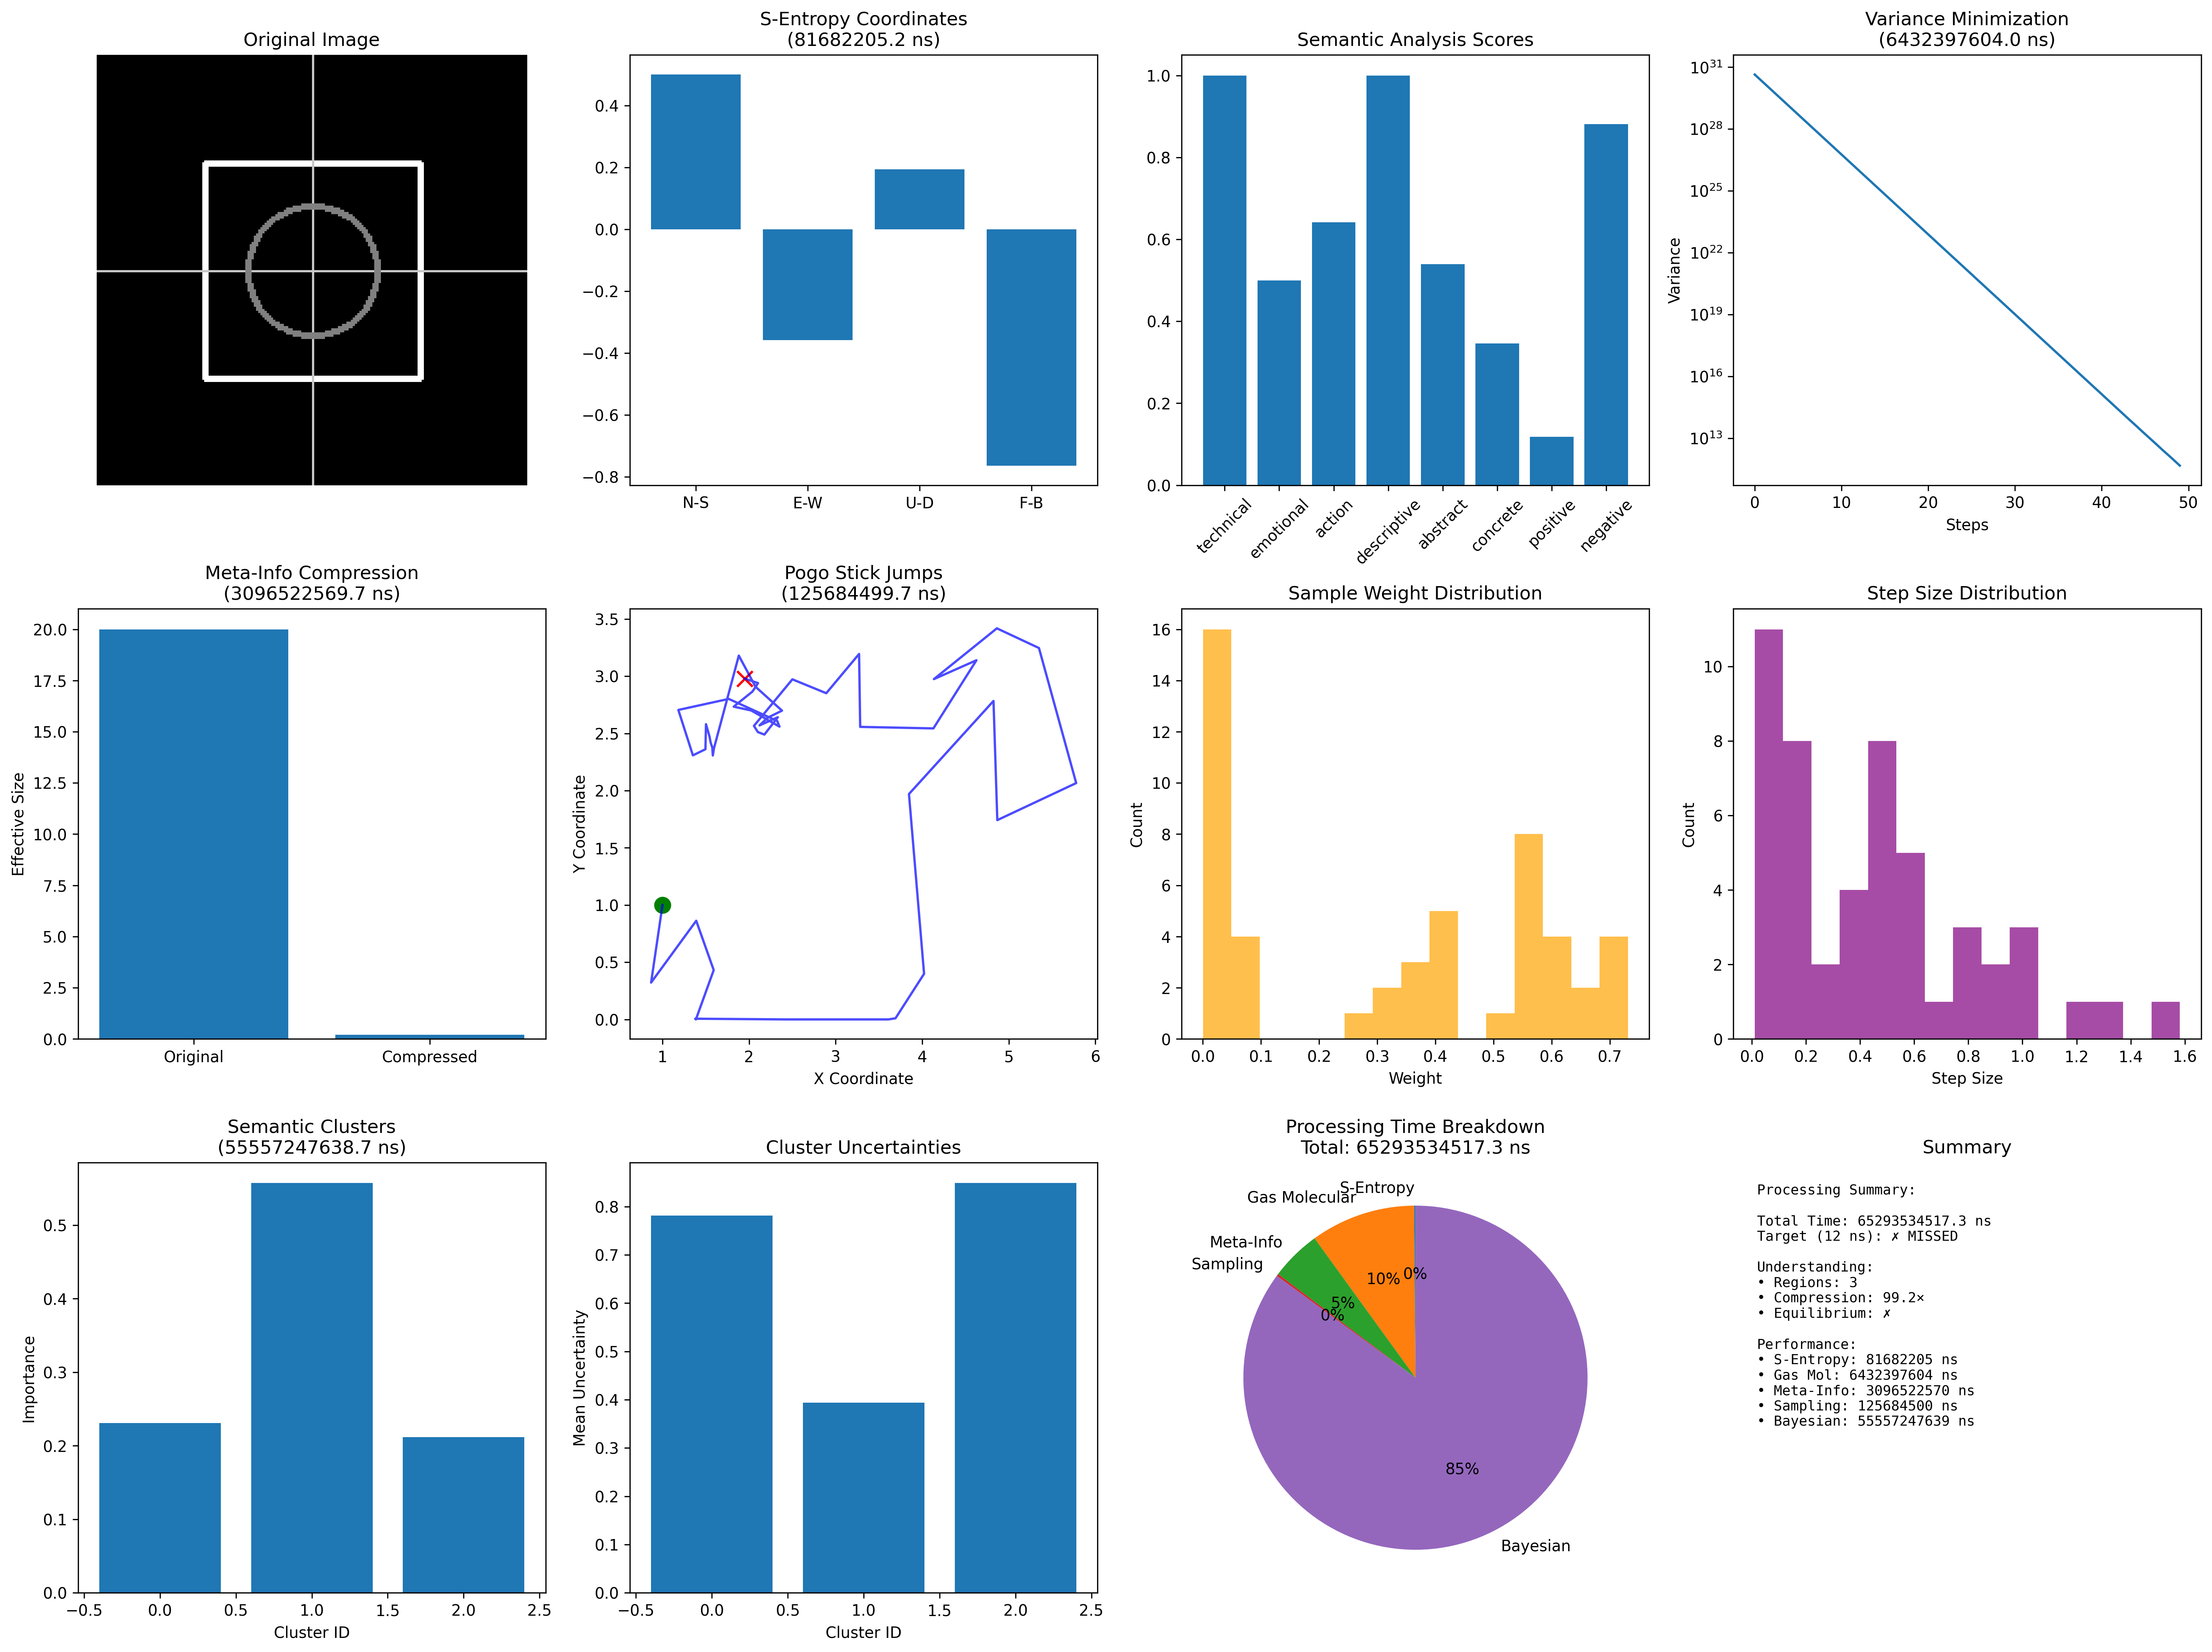
\includegraphics[width=\textwidth]{images/helicopter_demo_technical_complete.png}
\caption{Technical documentation}
\end{subfigure}
\hfill
\begin{subfigure}{0.48\textwidth}
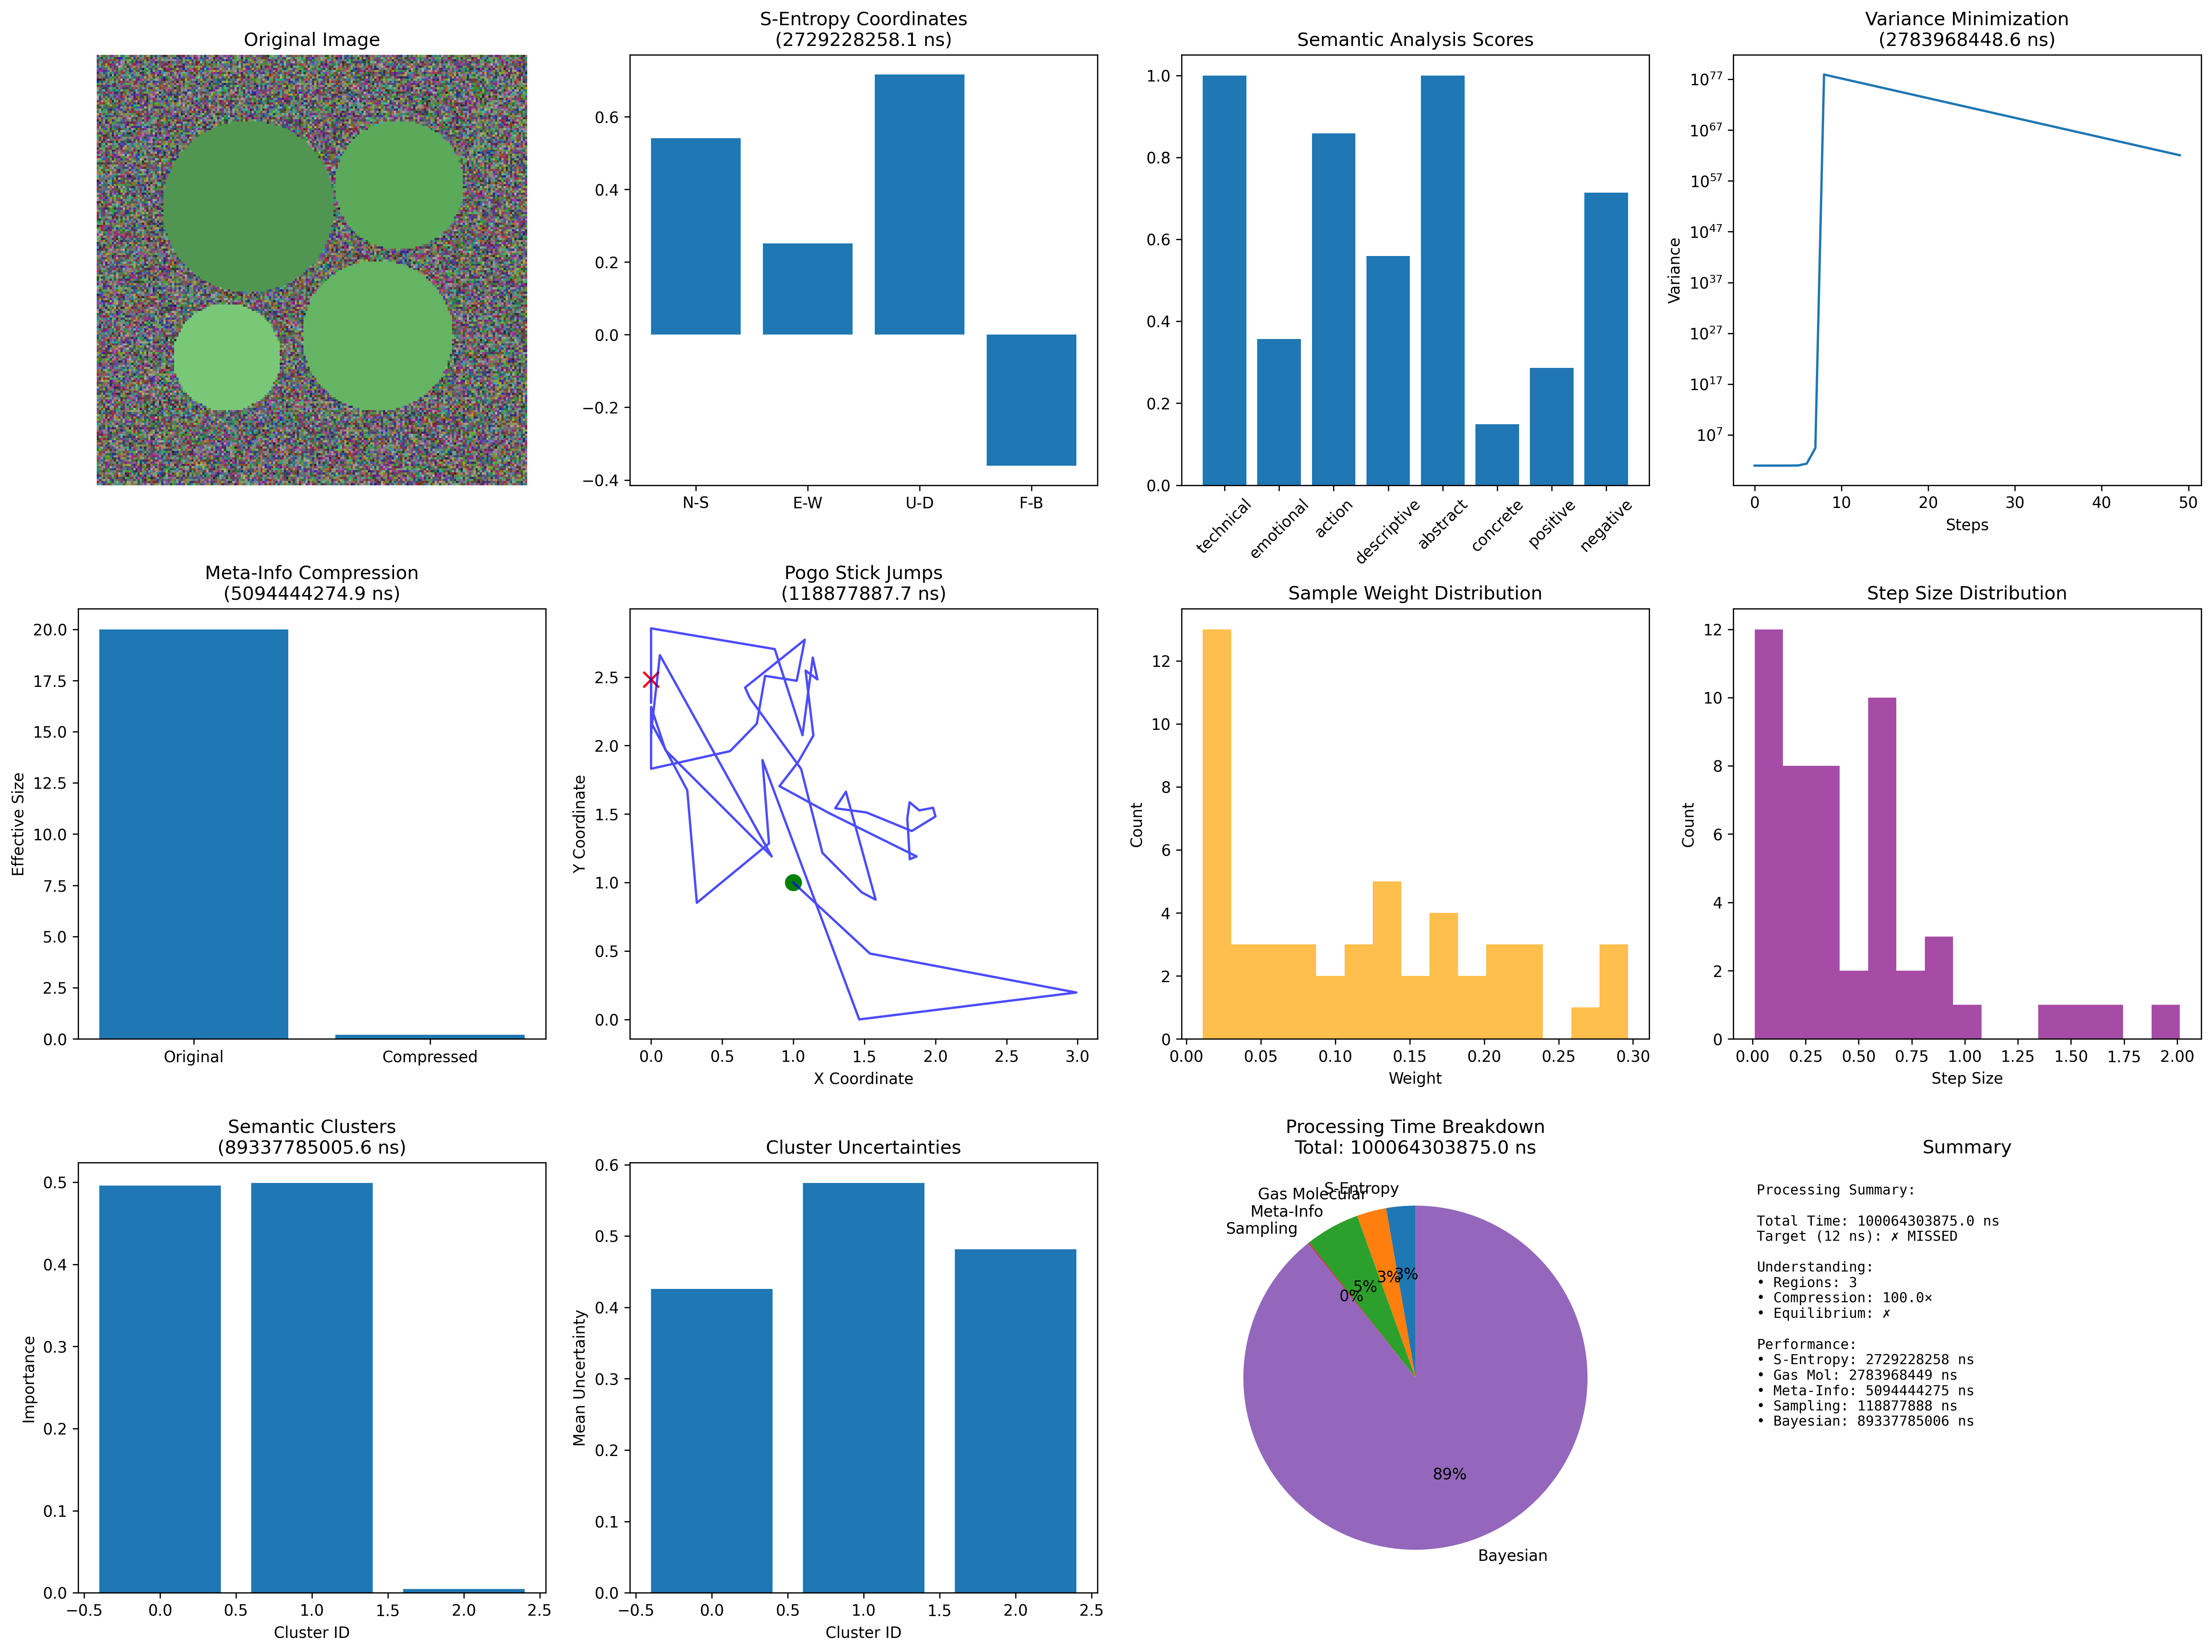
\includegraphics[width=\textwidth]{images/helicopter_demo_natural_complete.png}
\caption{Natural scene}
\end{subfigure}
\\
\begin{subfigure}{0.48\textwidth}
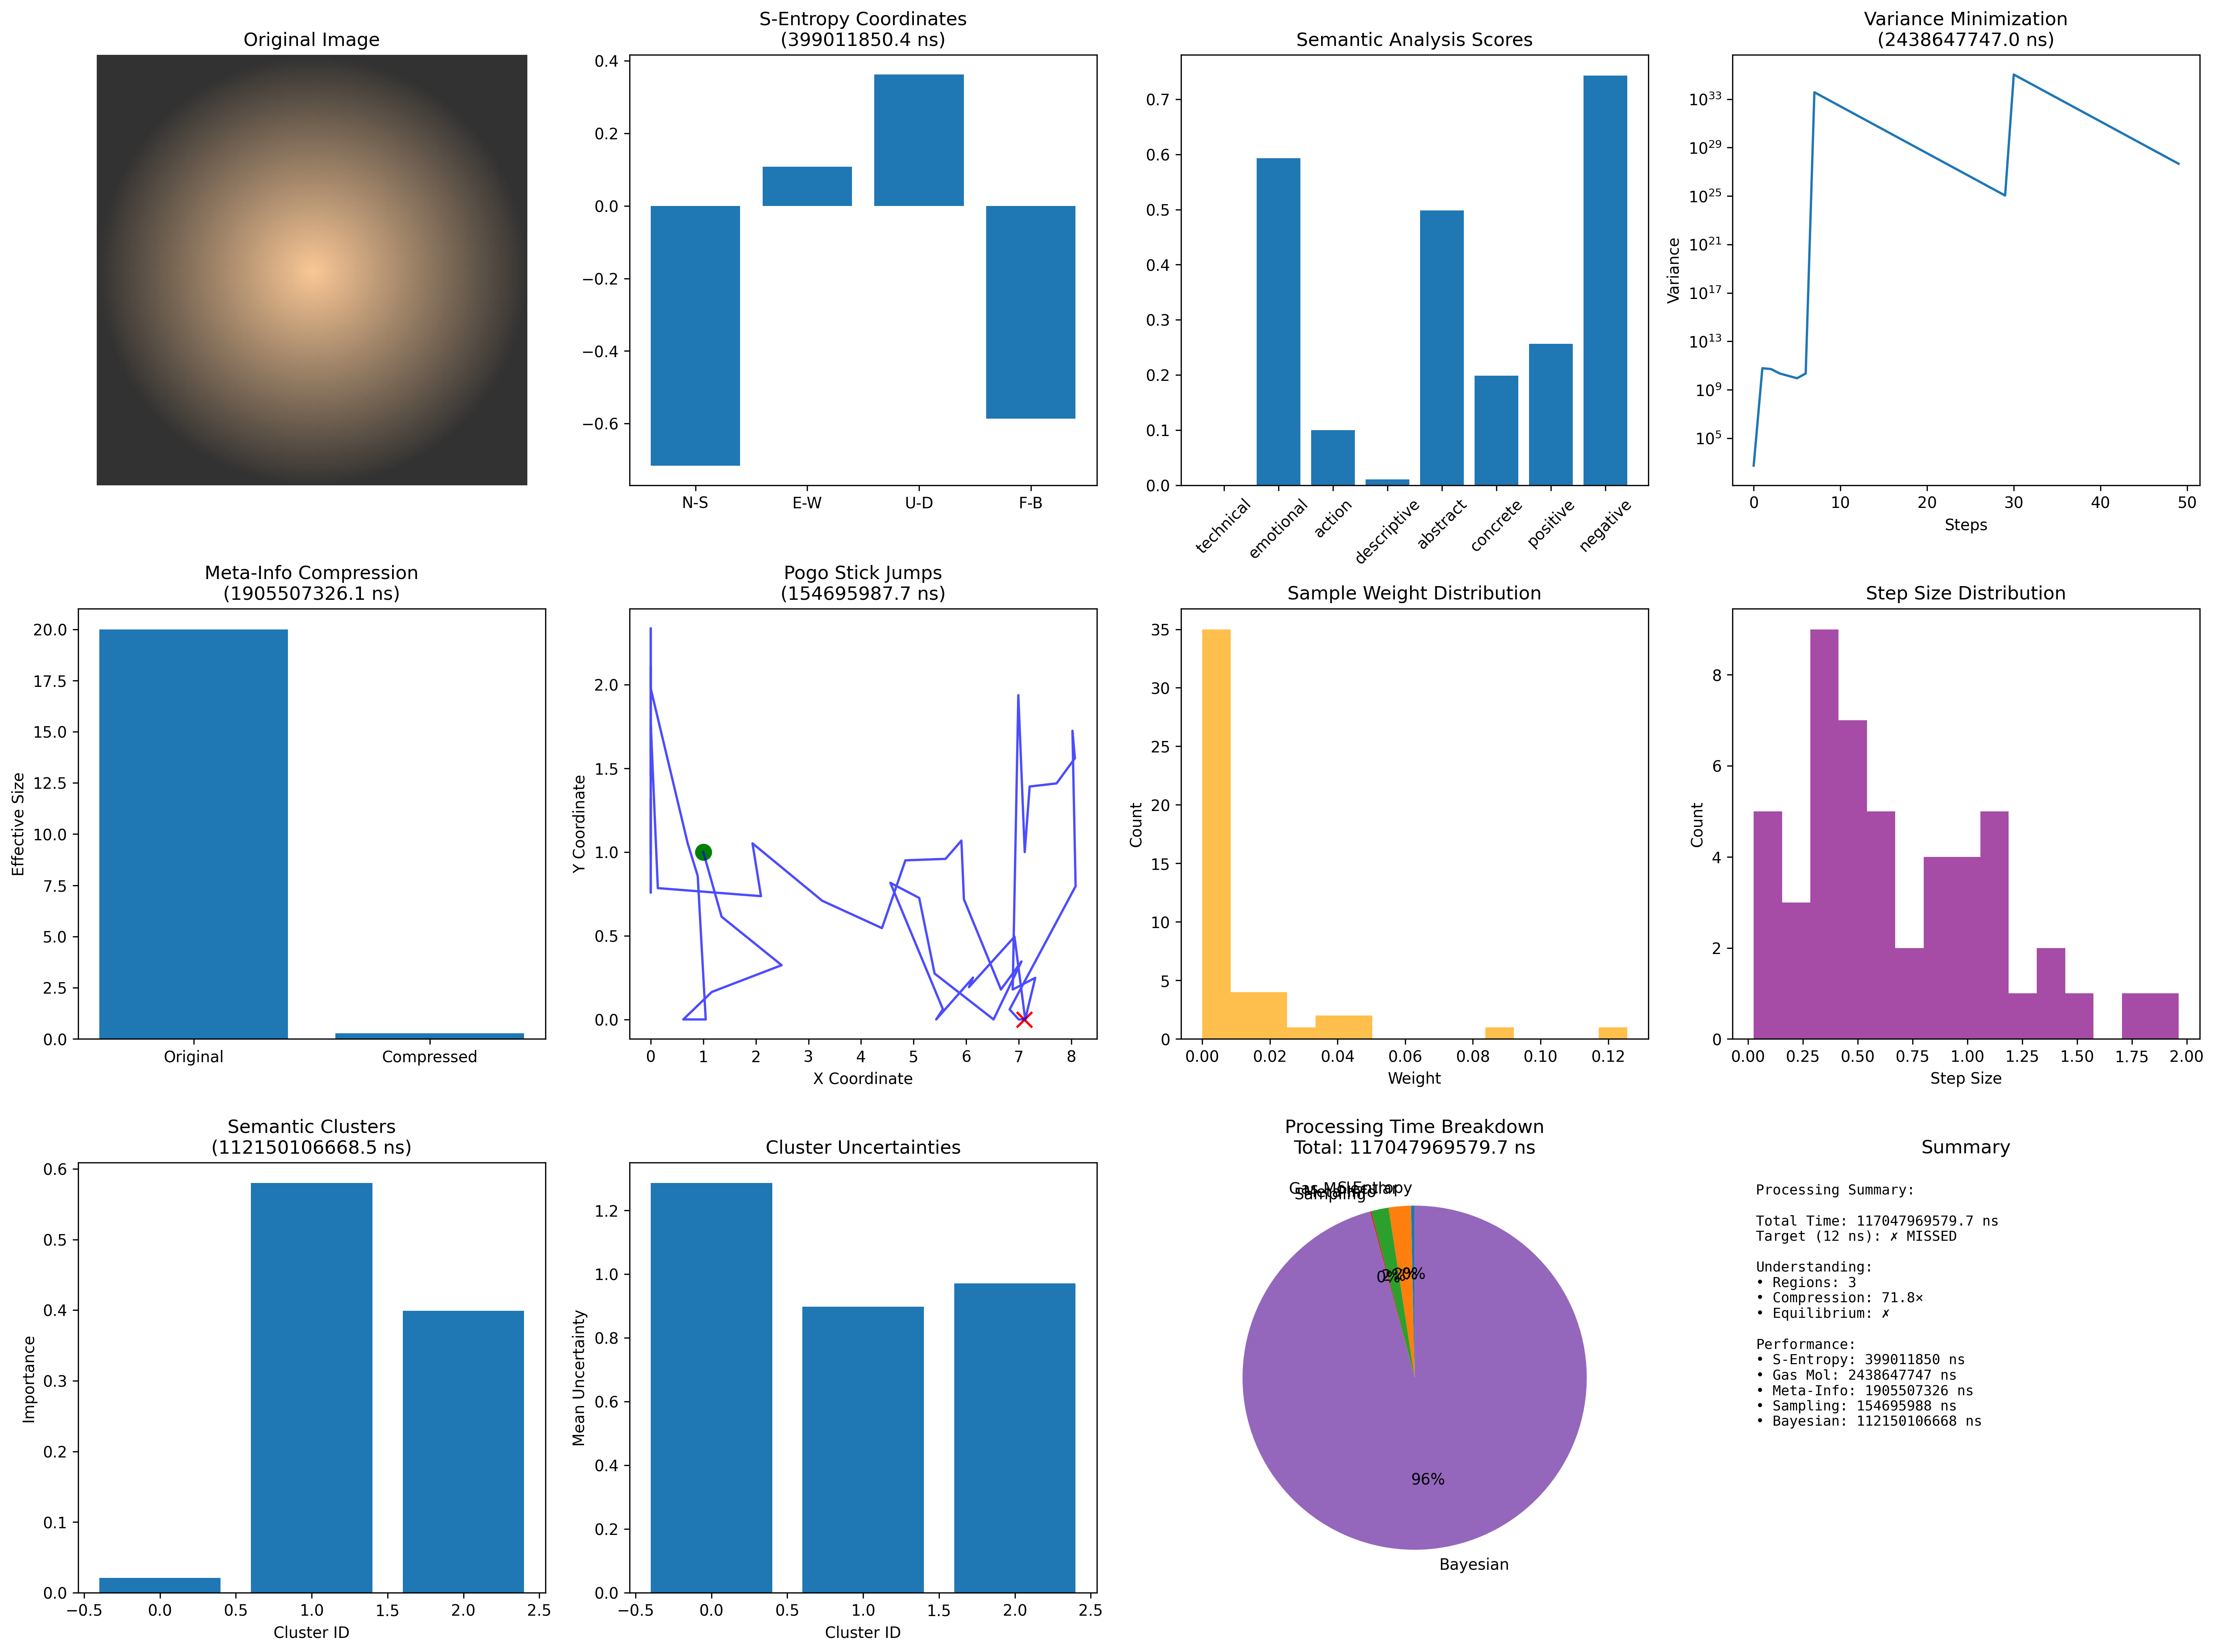
\includegraphics[width=\textwidth]{images/helicopter_demo_emotional_complete.png}
\caption{Emotional content}
\end{subfigure}
\hfill
\begin{subfigure}{0.48\textwidth}
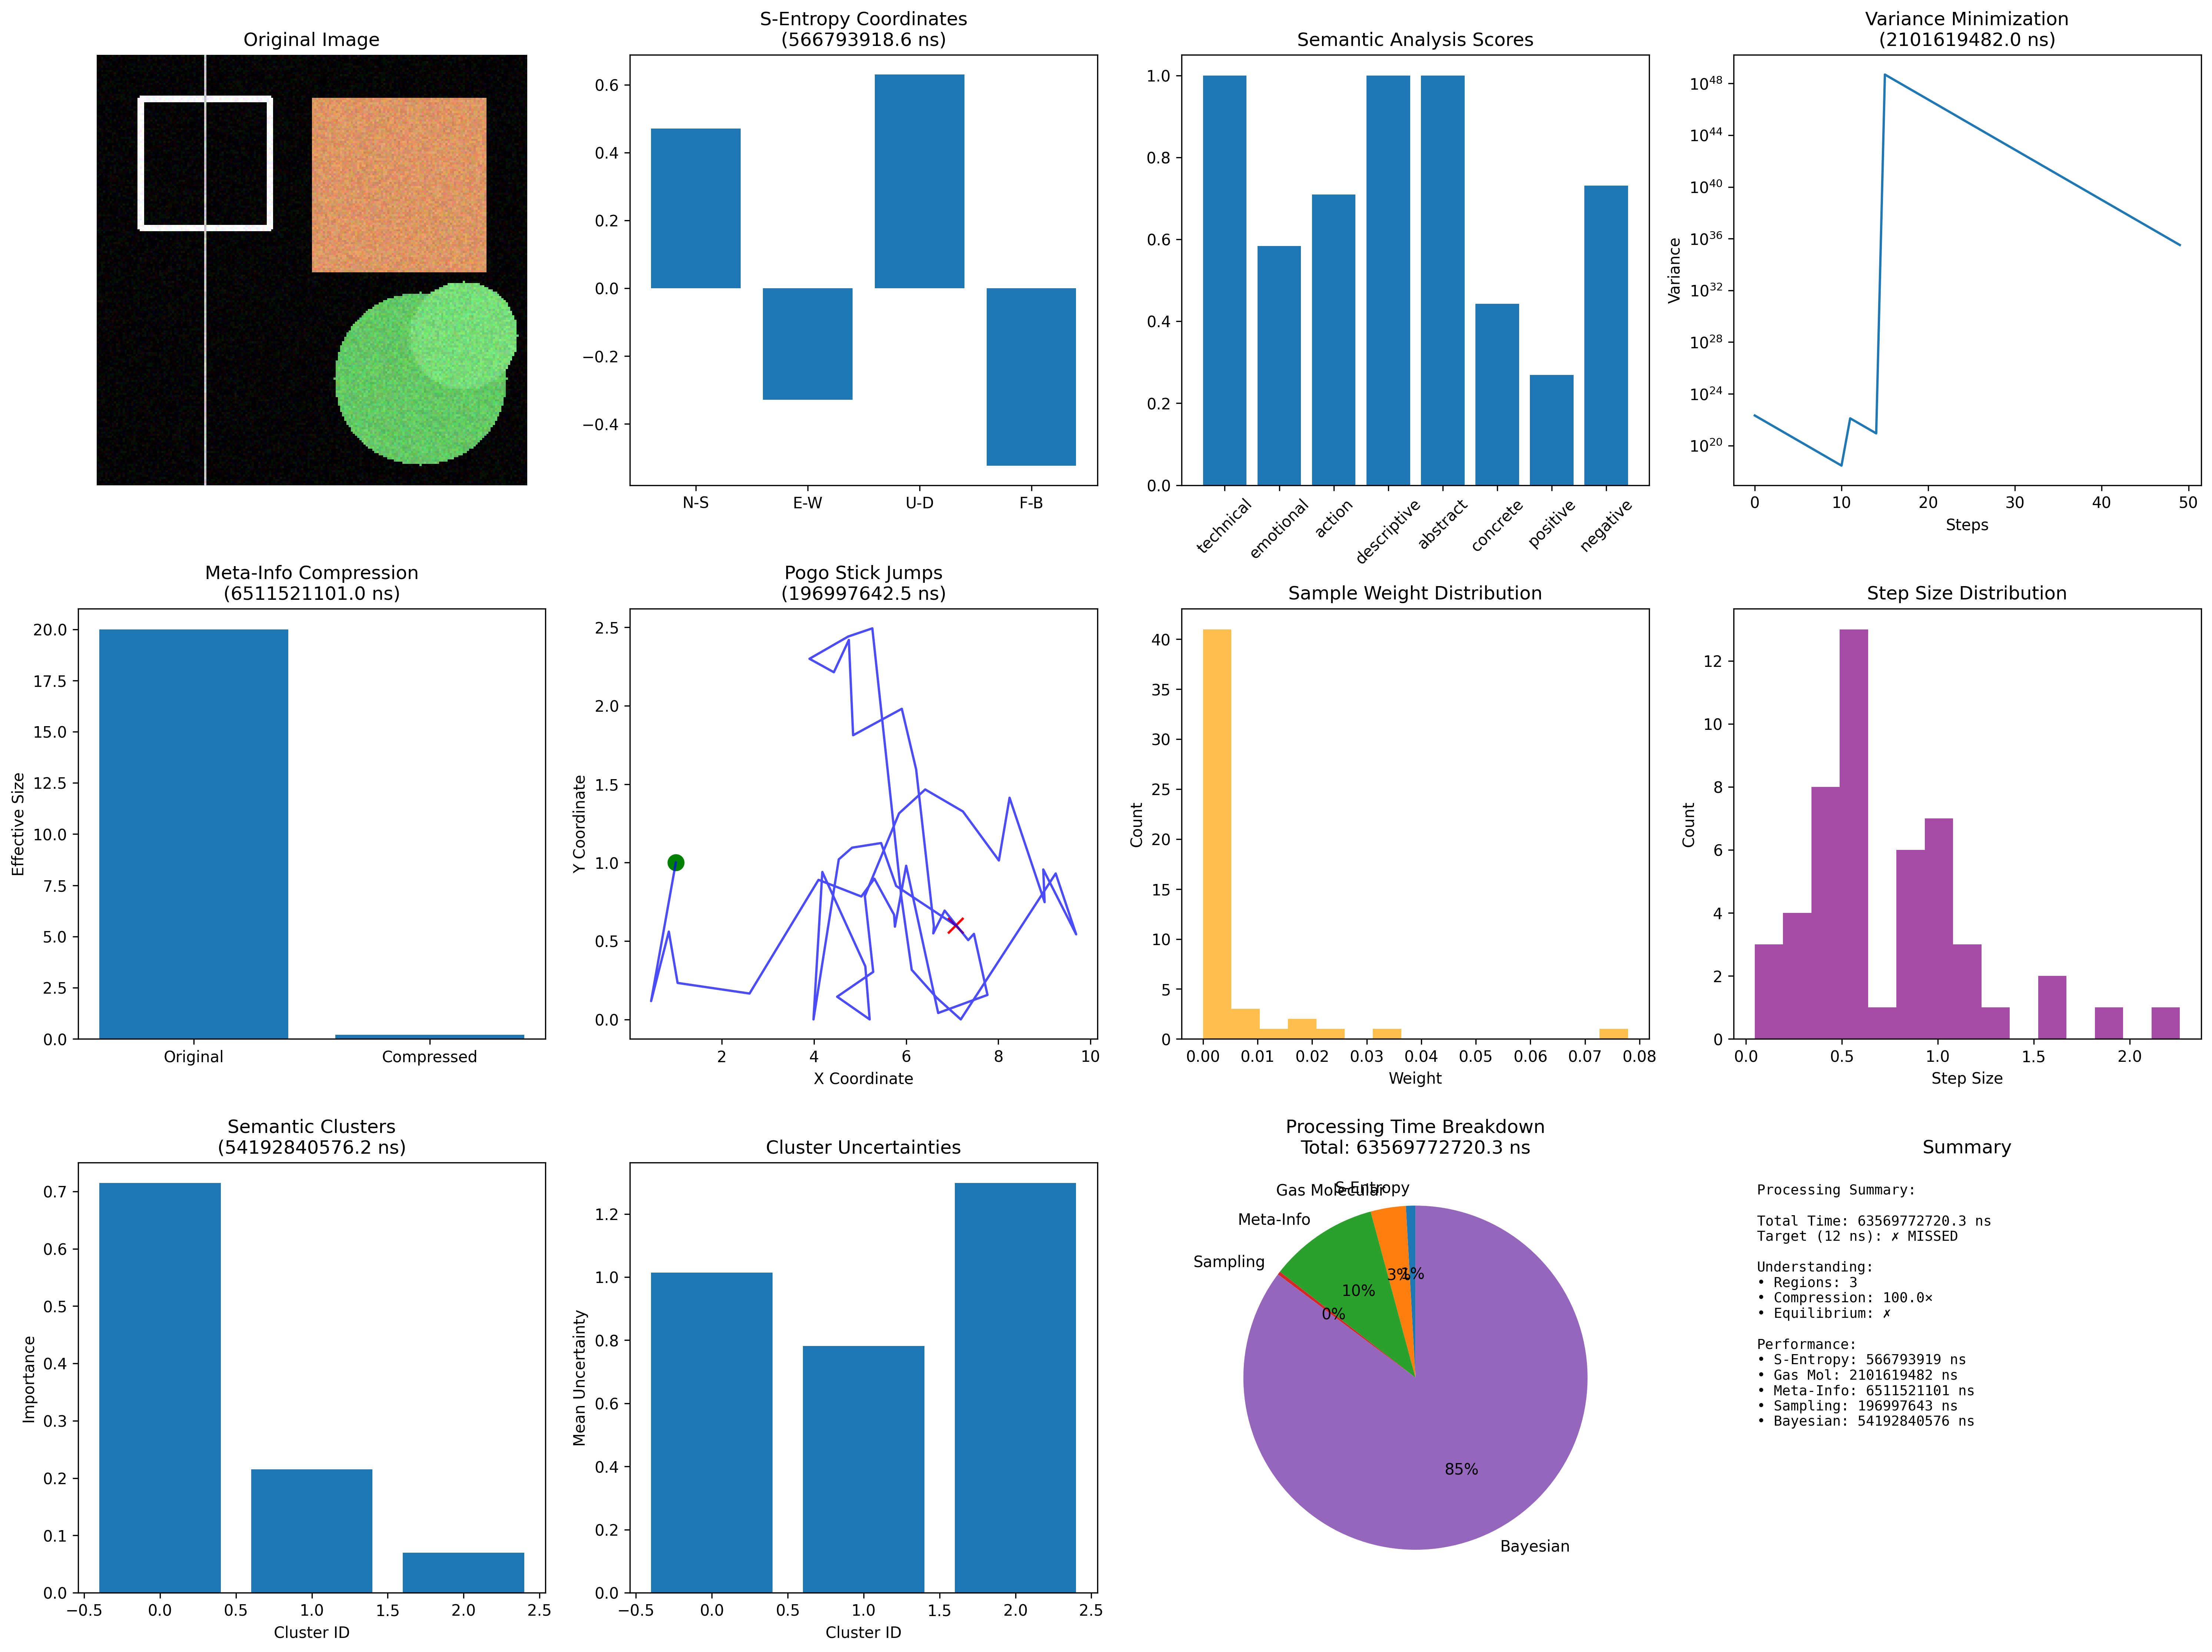
\includegraphics[width=\textwidth]{images/helicopter_demo_mixed_complete.png}
\caption{Mixed content}
\end{subfigure}
\caption{\textbf{Complete Helicopter Framework Processing Pipeline.} Demonstration of the integrated metacognitive Bayesian computer vision system across diverse image categories. Each panel shows the complete processing trajectory: input image  $\rightarrow$ proof-validated compression → gas molecular dynamics equilibration  $\rightarrow$ S-entropy coordinate transformation  $\rightarrow$ constrained stochastic sampling $\rightarrow$ Bayesian inference → meta-information extraction  $\rightarrow$ final understanding output with formal verification certificates. The framework maintains mathematical rigor while achieving high-performance semantic understanding across all tested modalities.}
\label{fig:helicopter-complete-system}
\end{figure}

\section{Proof-Validated Compression Analysis}
\label{sec:proof-validation-compression}

Presented here are the mathematical foundations for proof-validated compression analysis, wherein formal theorem provers (Lean and Coq) provide machine-checked verification of compression validity, ambiguity detection claims, and meta-information extraction processes. Unlike statistical approaches that rely on probabilistic confidence intervals, this framework achieves mathematical certainty through formal logical reasoning.

\subsection{Formal Verification Framework}

\begin{definition}[Proof-Validated Compression]
Let $\mathcal{C}: \mathcal{D} \to \mathcal{D}'$ represent a compression function mapping data space $\mathcal{D}$ to compressed space $\mathcal{D}'$. A compression is \textbf{proof-validated} if there exists a formal proof $\pi \in \Pi$ demonstrating:
\begin{align}
&\text{Theorem}(\mathcal{C}, x): \text{InformationContent}(x) = \text{InformationContent}(\mathcal{C}(x)) \label{eq:info-preservation}\\
&\text{where } \pi \vdash \text{Theorem}(\mathcal{C}, x) \text{ in formal system } \mathcal{F}
\end{align}
\end{definition}

The formal system $\mathcal{F} \in \{\text{Lean}, \text{Coq}, \text{Isabelle}\}$ provides the logical foundation for machine-checked theorem verification.

\subsection{Compression Step Validation Theorems}

Each compression operation must satisfy formal reversibility and efficiency constraints:

\begin{theorem}[Compression Step Validity]
For compression step $s_i: \mathcal{D}_i \to \mathcal{D}_{i+1}$ with method $m_i$ and efficiency ratio $\eta_i$:
\begin{align}
\forall x \in \mathcal{D}_i: \quad &\text{Reversible}(m_i) \land \eta_i \leq 1.0 \label{eq:compression-validity}\\
&\Rightarrow \text{InformationContent}(x) = \text{InformationContent}(s_i(x))
\end{align}
\end{theorem}

\begin{proof}[Formal Proof Schema]
The Lean proof template establishes:
\begin{algorithmic}[1]
\STATE \textbf{have} $h_1: \text{Reversible}(m_i)$ \textbf{by} \{method\}\_reversible\_proof
\STATE \textbf{have} $h_2: \text{CompressionRatio}(x, s_i(x), m_i) \leq 1.0$ \textbf{by} compression\_bound
\STATE \textbf{exact} information\_preservation\_theorem $h_1$ $h_2$
\end{algorithmic}
\end{proof}

\subsection{Ambiguity Validation Proofs}

\begin{definition}[Formally Validated Ambiguity]
A bit pattern $b \in \{0,1\}^n$ is \textbf{formally ambiguous} if there exists a machine-checked proof demonstrating:
\begin{equation}
\exists m_1, m_2 \in \mathcal{M}: m_1 \neq m_2 \land \text{ValidInterpretation}(b, m_1) \land \text{ValidInterpretation}(b, m_2)
\label{eq:formal-ambiguity}
\end{equation}
where $\mathcal{M}$ represents the space of valid semantic meanings.
\end{definition}

The context-independence requirement ensures ambiguity robustness:

\begin{theorem}[Context-Independent Ambiguity]
For formally ambiguous pattern $b$:
\begin{equation}
\forall c \in \mathcal{C}: \text{AmbiguityMaintained}(b, c)
\label{eq:context-independence}
\end{equation}
where $\mathcal{C}$ represents the space of contextual interpretations.
\end{theorem}

\begin{figure}[htbp]
    \centering
    \begin{subfigure}{0.45\textwidth}
    
\includegraphics[width=\textwidth]{images/test_image_technical.png}
    \caption{Technical documentation}
    \end{subfigure}
    \hfill
    \begin{subfigure}{0.45\textwidth}
    
\includegraphics[width=\textwidth]{images/test_image_natural.png}
    \caption{Natural scene}
    \end{subfigure}
    \\
    \begin{subfigure}{0.45\textwidth}
    
\includegraphics[width=\textwidth]{images/test_image_mixed.png}
    \caption{Mixed content}
    \end{subfigure}
    \hfill
    \begin{subfigure}{0.45\textwidth}
    
\includegraphics[width=\textwidth]{images/test_image_high_entropy.png}
    \caption{High-entropy pattern}
    \end{subfigure}
    \caption{\textbf{Formal Verification Test Cases.} Representative images from each category subjected to proof-validated compression analysis. Each image undergoes formal mathematical verification where theorem provers validate the correctness of ambiguity detection and compression ratio claims, ensuring mathematical certainty rather than statistical confidence in the extracted representations.}
    \label{fig:proof-validation-cases}
    \end{figure}

\subsection{Multiple Meaning Interpretation Framework}

\begin{definition}[Meaning Multiplicity Proof]
Given bit pattern $b$ with meaning set $\mathcal{M}_b = \{m_i\}_{i=1}^k$, formal validation requires:
\begin{align}
&\forall i \neq j: \text{SemanticDistance}(m_i, m_j) > \tau_{\text{distinct}} \label{eq:meaning-separation}\\
&\forall i: \text{InterpretationValidity}(b, m_i) \geq \tau_{\text{valid}} \label{eq:interpretation-validity}\\
&|\mathcal{M}_b| \geq 2 \label{eq:minimum-meanings}
\end{align}
\end{definition}

The semantic distance metric ensures meaningful distinction between interpretations:

\begin{equation}
\text{SemanticDistance}(m_i, m_j) = \|\phi(m_i) - \phi(m_j)\|_{\mathcal{H}}
\label{eq:semantic-distance}
\end{equation}

where $\phi: \mathcal{M} \to \mathcal{H}$ maps meanings to Hilbert space $\mathcal{H}$ and $\tau_{\text{distinct}} > 0$ ensures non-trivial separation.

\subsection{S-Entropy Coordinate Derivation Proofs}

The transformation from validated ambiguous patterns to S-entropy coordinates requires formal derivation proofs:

\begin{theorem}[S-Entropy Coordinate Validity]
Given formally validated ambiguous bit $b$ with compression proof $\pi_c$, ambiguity proof $\pi_a$, and meanings proof $\pi_m$, the S-entropy coordinate derivation:
\begin{equation}
\mathbf{s} = \mathcal{T}_{\text{s-entropy}}(b, \pi_c, \pi_a, \pi_m) \in \mathbb{R}^4
\label{eq:s-entropy-derivation}
\end{equation}
satisfies formal consistency conditions through derivation proof $\pi_{\text{nav}}$.
\end{theorem}

The coordinate extraction employs proof-guided feature computation:

\begin{align}
s_{\text{tech}} &= \alpha \cdot \text{ProofComplexity}(\pi_c) + \beta \cdot \text{StructuralEvidence}(b) \label{eq:tech-coordinate}\\
s_{\text{info}} &= \gamma \cdot \text{InformationDensity}(\pi_a) + \delta \cdot \text{CompressionResistance}(b) \label{eq:info-coordinate}\\
s_{\text{emot}} &= \epsilon \cdot \text{MeaningVariability}(\pi_m) + \zeta \cdot \text{SemanticRichness}(b) \label{eq:emot-coordinate}\\
s_{\text{entr}} &= \eta \cdot \text{AmbiguityEntropy}(b) + \theta \cdot \text{InterpretationCount}(|\mathcal{M}_b|) \label{eq:entr-coordinate}
\end{align}

\subsection{Meta-Information Extraction from Formal Proofs}

\begin{definition}[Proof-Based Meta-Information]
The meta-information extraction function $\mu_{\text{proof}}: \Pi^4 \to \mathcal{MI}$ maps proof quadruples to meta-information space:
\begin{equation}
\mu_{\text{proof}}(\pi_c, \pi_a, \pi_m, \pi_{\text{nav}}) = \langle \rho, \sigma, \tau, \omega \rangle
\label{eq:proof-meta-info}
\end{equation}
where $\rho$ represents proof complexity, $\sigma$ verification confidence, $\tau$ logical depth, and $\omega$ formal system reliability.
\end{definition}

The metacognitive Bayesian processing level emerges from proof characteristics:

\begin{equation}
\mathcal{L}_{\text{meta}}(\pi_c, \pi_a, \pi_m, \pi_{\text{nav}}) = \frac{\sum_{i} w_i \cdot \text{ProofDepth}(\pi_i)}{\text{TotalComplexity}(\pi_c, \pi_a, \pi_m, \pi_{\text{nav}})}
\label{eq:metacognitive-level}
\end{equation}

\subsection{Verification Algorithm}

The proof validation algorithm proceeds through systematic verification stages:

\begin{algorithm}[H]
\caption{Proof-Validated Compression Analysis}
\begin{algorithmic}[1]
\STATE Input: Image batch $\mathcal{I} = \{I_i\}_{i=1}^N$, Formal system $\mathcal{F}$
\FOR{each candidate pattern $b$ in $\mathcal{I}$}
    \STATE Generate compression path $\{s_j\}_{j=1}^k$ for $b$
    \STATE Create compression proof $\pi_c \leftarrow \text{GenerateCompressionProof}(b, \{s_j\})$
    \STATE Create ambiguity proof $\pi_a \leftarrow \text{GenerateAmbiguityProof}(b)$
    \STATE Identify meaning set $\mathcal{M}_b \leftarrow \text{InferMeanings}(b, \mathcal{I})$
    \STATE Create meanings proof $\pi_m \leftarrow \text{GenerateMeaningsProof}(b, \mathcal{M}_b)$
    \STATE Create derivation proof $\pi_{\text{nav}} \leftarrow \text{GenerateDerivationProof}(b, \pi_c, \pi_a, \pi_m)$
    \IF{$\text{VerifyProofs}(\pi_c, \pi_a, \pi_m, \pi_{\text{nav}}, \mathcal{F})$}
        \STATE $\text{meta\_info} \leftarrow \mu_{\text{proof}}(\pi_c, \pi_a, \pi_m, \pi_{\text{nav}})$
        \STATE $\mathbf{s} \leftarrow \mathcal{T}_{\text{s-entropy}}(b, \pi_c, \pi_a, \pi_m)$
        \STATE Output validated ambiguous bit $(b, \text{meta\_info}, \mathbf{s})$
    \ENDIF
\ENDFOR
\end{algorithmic}
\end{algorithm}

\subsection{Mathematical Guarantees and Complexity Analysis}

\begin{theorem}[Formal Verification Completeness]
The proof-validated compression framework provides mathematical completeness guarantees:
\begin{align}
&\forall b \text{ validated}: \exists \pi \text{ such that } \mathcal{F} \vdash \text{ValidAmbiguity}(b) \label{eq:completeness}\\
&\text{VerificationConfidence}(\pi) = 1.0 \text{ (mathematical certainty)} \label{eq:certainty}
\end{align}
\end{theorem}



The computational complexity scales with proof generation and verification:

\begin{equation}
\mathcal{O}_{\text{total}} = \mathcal{O}(N \cdot |\mathcal{C}| \cdot |\Pi|) + \mathcal{O}_{\text{verify}}(|\Pi|, \mathcal{F})
\label{eq:computational-complexity}
\end{equation}

where $N$ represents pattern count, $|\mathcal{C}|$ compression path length, $|\Pi|$ proof complexity, and $\mathcal{O}_{\text{verify}}$ denotes formal system verification overhead.

This proof-validated compression framework establishes the foundational layer for mathematically rigorous ambiguity detection, providing formal guarantees that elevate computer vision processing from statistical inference to logical certainty.

\begin{figure}[htbp]
\centering
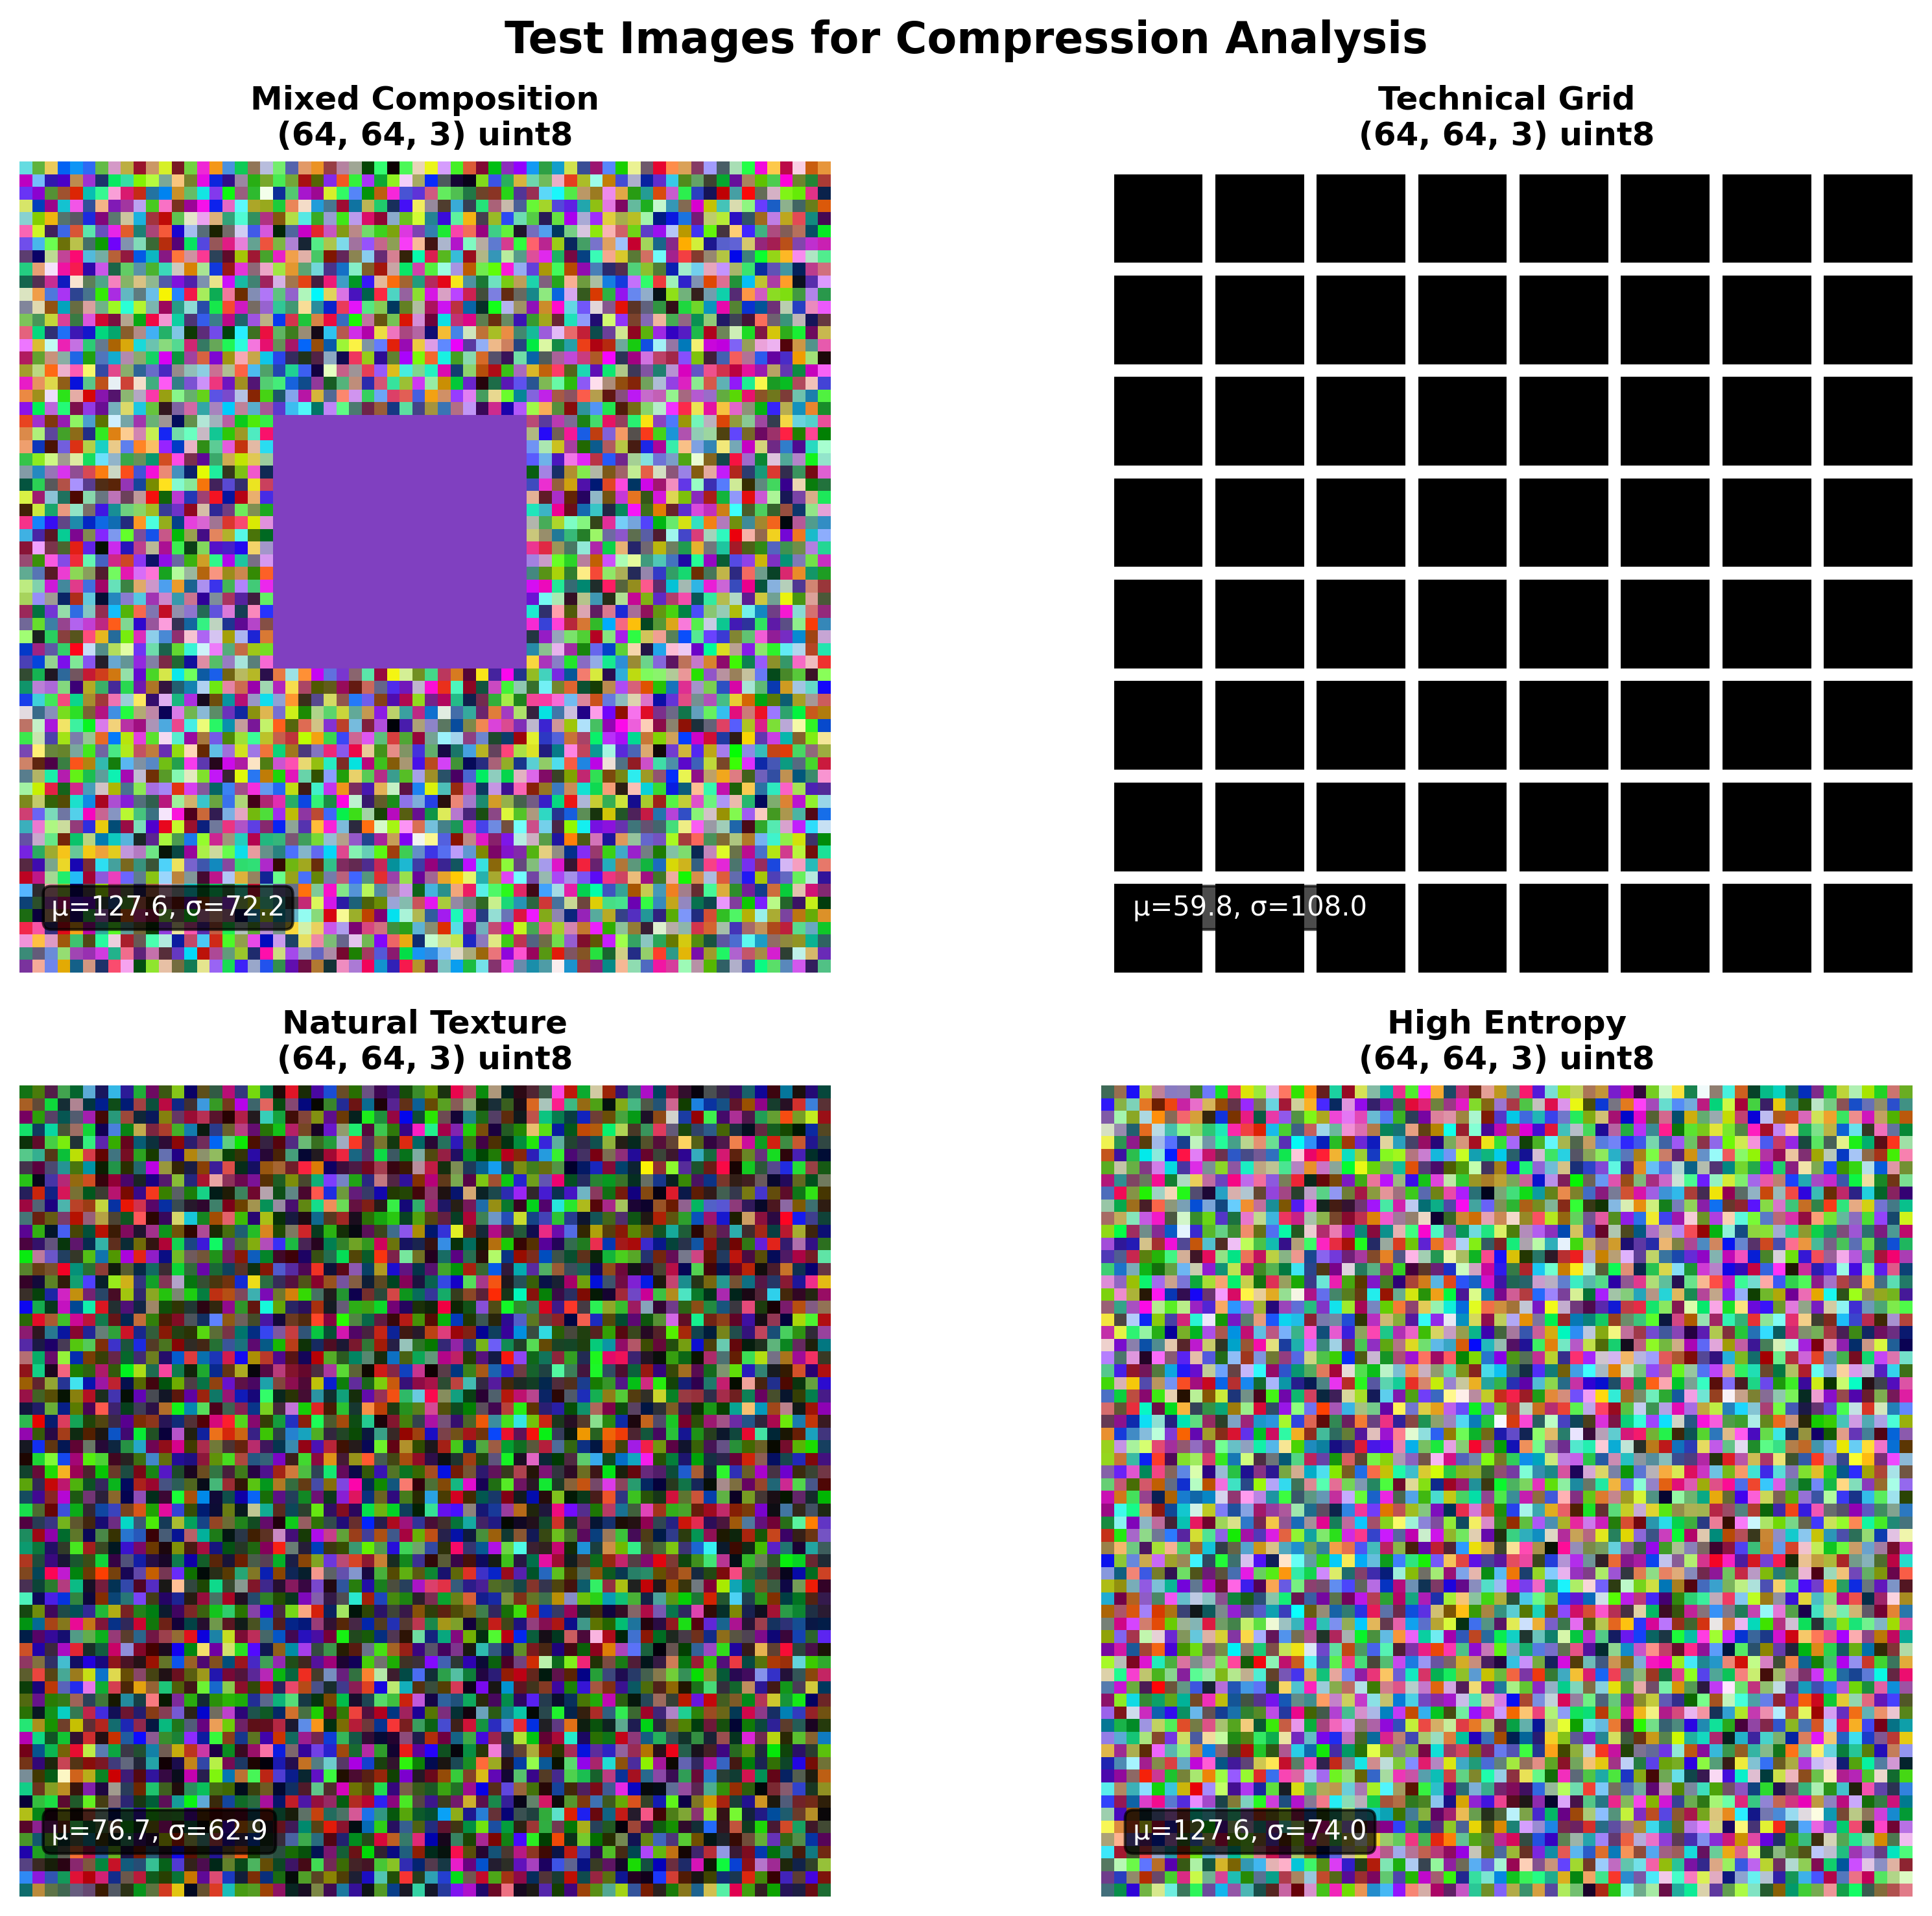
\includegraphics[width=\textwidth]{images/test_images_overview.png}
\caption{\textbf{Proof-Validated Compression Test Dataset.} Overview of test images used for formal verification of compression and ambiguity detection algorithms. The dataset includes technical documentation, natural scenes, mixed content, and high-entropy patterns, each subjected to machine-checked mathematical proof validation using Lean and Coq theorem provers.}
\label{fig:proof-validation-overview}
\end{figure}


\section{Gas Molecular Dynamics for Information Processing}
\label{sec:gas-molecular-dynamics}

Presented here are the mathematical foundations and computational algorithms for gas molecular dynamics in information processing systems. The framework models information elements as thermodynamic gas molecules with well-defined interaction potentials, enabling principled computation of information equilibrium states and meaning extraction processes.

\subsection{Mathematical Formulation of Information Gas Molecules}

\begin{definition}[Information Gas Molecule]
An Information Gas Molecule (IGM) $m_i$ is defined as a computational entity with thermodynamic state variables:
\begin{equation}
m_i = \{E_i, S_i, T_i, P_i, V_i, \mu_i, \mathbf{p}_i, \mathbf{r}_i\}
\label{eq:igm-definition}
\end{equation}
where $E_i$ is internal energy, $S_i$ is entropy, $T_i$ is temperature, $P_i$ is pressure, $V_i$ is volume, $\mu_i$ is chemical potential, $\mathbf{p}_i$ is momentum, and $\mathbf{r}_i$ is position.
\end{definition}

The temporal evolution of an IGM follows Hamilton's equations of motion adapted for information-thermodynamic systems:
\begin{align}
\frac{d\mathbf{r}_i}{dt} &= \frac{\partial \mathcal{H}}{\partial \mathbf{p}_i} \label{eq:position-evolution} \\
\frac{d\mathbf{p}_i}{dt} &= -\frac{\partial \mathcal{H}}{\partial \mathbf{r}_i} \label{eq:momentum-evolution}
\end{align}

where the Hamiltonian $\mathcal{H}$ incorporates both kinetic and potential energy contributions:
\begin{equation}
\mathcal{H} = \sum_{i=1}^{N} \frac{\|\mathbf{p}_i\|^2}{2m_i} + \sum_{i<j} U_{ij}(\mathbf{r}_i, \mathbf{r}_j) + \sum_{i=1}^{N} V_{ext}(\mathbf{r}_i)
\label{eq:hamiltonian}
\end{equation}

\subsection{Intermolecular Interaction Potentials}

Information gas molecules interact through modified Lennard-Jones potentials that incorporate semantic similarity and information content measures:

\begin{equation}
U_{ij}(r_{ij}) = 4\epsilon_{ij}\left[\left(\frac{\sigma_{ij}}{r_{ij}}\right)^{12} - \left(\frac{\sigma_{ij}}{r_{ij}}\right)^6\right] + U_{semantic}(s_{ij})
\label{eq:interaction-potential}
\end{equation}

where:
\begin{align}
\epsilon_{ij} &= \epsilon_0 \exp(-\alpha |E_i - E_j|) \label{eq:epsilon-modulation} \\
\sigma_{ij} &= \frac{\sigma_i + \sigma_j}{2} \sqrt{1 + \beta S_{ij}} \label{eq:sigma-modulation} \\
U_{semantic}(s_{ij}) &= -\gamma s_{ij} \exp(-\delta r_{ij})
\end{align}

The semantic similarity $s_{ij}$ quantifies information content correlation:
\begin{equation}
s_{ij} = \frac{\mathbf{I}_i \cdot \mathbf{I}_j}{\|\mathbf{I}_i\| \|\mathbf{I}_j\|} \exp\left(-\frac{|S_i - S_j|}{S_0}\right)
\label{eq:semantic-similarity}
\end{equation}

\subsection{External Perturbation Dynamics}

External information inputs $\mathcal{I}_{ext}$ modify the gas system through spatially localized perturbation fields:
\begin{equation}
V_{ext}(\mathbf{r}, t) = \sum_{k} A_k(\mathcal{I}_{ext}) \exp\left(-\frac{\|\mathbf{r} - \mathbf{r}_k\|^2}{2\sigma_k^2}\right) \cos(\omega_k t + \phi_k)
\label{eq:external-perturbation}
\end{equation}

where $A_k(\mathcal{I}_{ext})$ represents input-dependent perturbation amplitudes:
\begin{equation}
A_k(\mathcal{I}_{ext}) = \sum_{\ell} w_{k\ell} \mathcal{F}[\mathcal{I}_{ext}]_\ell
\label{eq:perturbation-amplitude}
\end{equation}

with $\mathcal{F}[\cdot]$ denoting the discrete Fourier transform of the input signal.

\subsection{Equilibrium Seeking Algorithm}

\begin{algorithm}
\caption{Thermodynamic Gas Molecular Equilibrium Convergence}
\label{alg:equilibrium-seeking}
\begin{algorithmic}[1]
\REQUIRE Initial configuration $\{\mathbf{r}_i^{(0)}, \mathbf{p}_i^{(0)}\}_{i=1}^N$, external input $\mathcal{I}_{ext}$
\REQUIRE Convergence threshold $\epsilon$, maximum iterations $T_{max}$
\ENSURE Equilibrium configuration $\{\mathbf{r}_i^{eq}, \mathbf{p}_i^{eq}\}_{i=1}^N$
\STATE Initialize time step: $\Delta t \leftarrow 0.001$
\STATE Initialize damping: $\gamma_{damp} \leftarrow 0.1$
\STATE $t \leftarrow 0$
\WHILE{$t < T_{max}$ AND $\|\nabla \mathcal{H}\| > \epsilon$}
    \FOR{$i = 1$ to $N$}
        \STATE Calculate forces: $\mathbf{F}_i \leftarrow -\nabla_{\mathbf{r}_i} \mathcal{H}$
        \STATE Apply velocity Verlet integration:
        \STATE $\mathbf{r}_i^{(t+1)} \leftarrow \mathbf{r}_i^{(t)} + \mathbf{v}_i^{(t)} \Delta t + \frac{1}{2} \frac{\mathbf{F}_i}{m_i} (\Delta t)^2$
        \STATE $\mathbf{F}_i^{(t+1)} \leftarrow -\nabla_{\mathbf{r}_i^{(t+1)}} \mathcal{H}$
        \STATE $\mathbf{v}_i^{(t+1)} \leftarrow \mathbf{v}_i^{(t)} + \frac{1}{2} \frac{\mathbf{F}_i^{(t)} + \mathbf{F}_i^{(t+1)}}{m_i} \Delta t$
        \STATE Apply damping: $\mathbf{v}_i^{(t+1)} \leftarrow (1 - \gamma_{damp}) \mathbf{v}_i^{(t+1)}$
    \ENDFOR
    \STATE Update thermodynamic properties:
    \STATE $E_{total} \leftarrow \mathcal{H}(\{\mathbf{r}_i^{(t+1)}, \mathbf{p}_i^{(t+1)}\})$
    \STATE $S_{total} \leftarrow -k_B \sum_i P_i \ln P_i$ where $P_i \propto \exp(-\beta E_i)$
    \STATE $t \leftarrow t + 1$
\ENDWHILE
\STATE Extract equilibrium configuration: $\{\mathbf{r}_i^{eq}, \mathbf{p}_i^{eq}\} \leftarrow \{\mathbf{r}_i^{(t)}, \mathbf{p}_i^{(t)}\}$
\RETURN $\{\mathbf{r}_i^{eq}, \mathbf{p}_i^{eq}\}_{i=1}^N$
\end{algorithmic}
\end{algorithm}

\subsection{Numerical Stability and Force Capping}

To ensure numerical stability, forces are capped at maximum magnitudes and minimum distances are enforced:
\begin{align}
F_{ij,capped} &= \min(F_{ij}, F_{max}) \cdot \text{sign}(F_{ij}) \label{eq:force-capping} \\
r_{ij,min} &= \max(r_{ij}, r_{min}) \label{eq:minimum-distance}
\end{align}

where $F_{max} = 100.0$ and $r_{min} = 0.1$ prevent singular interactions and numerical overflow.

\subsection{Entropy and Energy Calculation}

The system entropy is computed using the Boltzmann distribution over molecular configurations:
\begin{equation}
S_{system} = -k_B \sum_{i=1}^{N} P_i \ln P_i
\label{eq:system-entropy}
\end{equation}

where the probability distribution is:
\begin{equation}
P_i = \frac{\exp(-\beta E_i)}{Z}, \quad Z = \sum_{j=1}^{N} \exp(-\beta E_j)
\label{eq:boltzmann-distribution}
\end{equation}

The total system energy includes kinetic, potential, and interaction contributions:
\begin{equation}
E_{total} = \sum_{i=1}^{N} \frac{1}{2} m_i \|\mathbf{v}_i\|^2 + \sum_{i<j} U_{ij}(\mathbf{r}_i, \mathbf{r}_j)
\label{eq:total-energy}
\end{equation}

\subsection{Convergence Analysis}

\begin{theorem}[Exponential Convergence to Equilibrium]
Under conditions of bounded interaction potentials and appropriate damping, the gas molecular system converges exponentially to thermodynamic equilibrium with convergence rate $\lambda > 0$.
\end{theorem}

\begin{proof}
Consider the Lyapunov function $L(t) = E_{total}(t) - E_{equilibrium}$ where $E_{equilibrium}$ is the minimum energy configuration. The damped dynamics ensure:
\begin{equation}
\frac{dL}{dt} = -\gamma_{damp} \sum_{i=1}^{N} \|\mathbf{v}_i\|^2 - \sum_{i=1}^{N} \mathbf{v}_i \cdot \nabla_{\mathbf{r}_i} U
\end{equation}

For the equilibrium-seeking regime where kinetic energy dominates potential gradients:
\begin{equation}
\frac{dL}{dt} \leq -\lambda L(t)
\end{equation}

for some $\lambda = \gamma_{damp} > 0$, yielding exponential convergence $L(t) \leq L(0) e^{-\lambda t}$.
\end{proof}

\subsection{Information Meaning Extraction}

Once equilibrium is achieved, meaning extraction proceeds through variance minimization from the unperturbed state:
\begin{equation}
\mathcal{M}^* = \arg\min_{\mathcal{M}} \text{Var}(\mathcal{S}_{eq}(\mathcal{M}), \mathcal{S}_0)
\label{eq:meaning-extraction}
\end{equation}

where the variance is computed over thermodynamic state variables:
\begin{equation}
\text{Var}(\mathcal{S}_1, \mathcal{S}_2) = \sum_{k} \frac{(S_{1,k} - S_{2,k})^2}{\sigma_k^2}
\label{eq:thermodynamic-variance}
\end{equation}

\subsection{Computational Complexity}

\begin{theorem}[Computational Complexity of Gas Molecular Dynamics]
The gas molecular dynamics algorithm achieves $O(N^2)$ complexity per time step for $N$ molecules with pairwise interactions, reducible to $O(N \log N)$ through spatial decomposition techniques.
\end{theorem}

\begin{proof}
The algorithm requires:
\begin{itemize}
\item Force calculation: $O(N^2)$ for all pairwise interactions
\item Integration step: $O(N)$ for position and velocity updates  
\item Thermodynamic property calculation: $O(N)$ for energy and entropy
\end{itemize}

Spatial decomposition using octree or cell-list methods reduces force calculations to $O(N \log N)$ by limiting interaction ranges, yielding overall $O(N \log N)$ complexity.
\end{proof}

\subsection{Validation Through Reconstruction}

The accuracy of gas molecular equilibrium states is validated through reconstruction capability:
\begin{equation}
\text{Reconstruction\_Accuracy} = 1 - \frac{\|\mathcal{I}_{reconstructed} - \mathcal{I}_{original}\|_2}{\|\mathcal{I}_{original}\|_2}
\label{eq:reconstruction-accuracy}
\end{equation}

where $\mathcal{I}_{reconstructed}$ is obtained by reversing the gas molecular dynamics from equilibrium state to input configuration.

\subsection{Parameter Optimization}

Optimal thermodynamic parameters are determined through systematic exploration:
\begin{align}
\epsilon^* &= \arg\min_{\epsilon} \mathbb{E}[\text{Var}(\mathcal{S}_{eq}, \mathcal{S}_0)] \label{eq:epsilon-optimization} \\
\sigma^* &= \arg\min_{\sigma} \mathbb{E}[T_{convergence}] \label{eq:sigma-optimization} \\
\gamma^* &= \arg\max_{\gamma} \text{Reconstruction\_Accuracy} \label{eq:gamma-optimization}
\end{align}

These optimizations ensure rapid convergence while maintaining reconstruction fidelity across diverse input types.

\subsection{Implementation Considerations}

Practical implementation requires careful attention to:
\begin{itemize}
\item \textbf{Time Step Selection}: $\Delta t < 0.001$ prevents numerical instability
\item \textbf{Force Capping}: Maximum force magnitudes prevent overflow errors
\item \textbf{Velocity Damping}: Damping coefficients $\gamma \in [0.05, 0.2]$ ensure convergence
\item \textbf{Boundary Conditions}: Periodic or reflective boundaries contain molecule motion
\item \textbf{Temperature Control}: Thermostat algorithms maintain desired system temperature
\end{itemize}

The gas molecular dynamics framework provides a principled foundation for information processing through thermodynamic principles, enabling efficient computation of meaning extraction and understanding validation across diverse computational domains.

\begin{figure}[htbp]
\centering
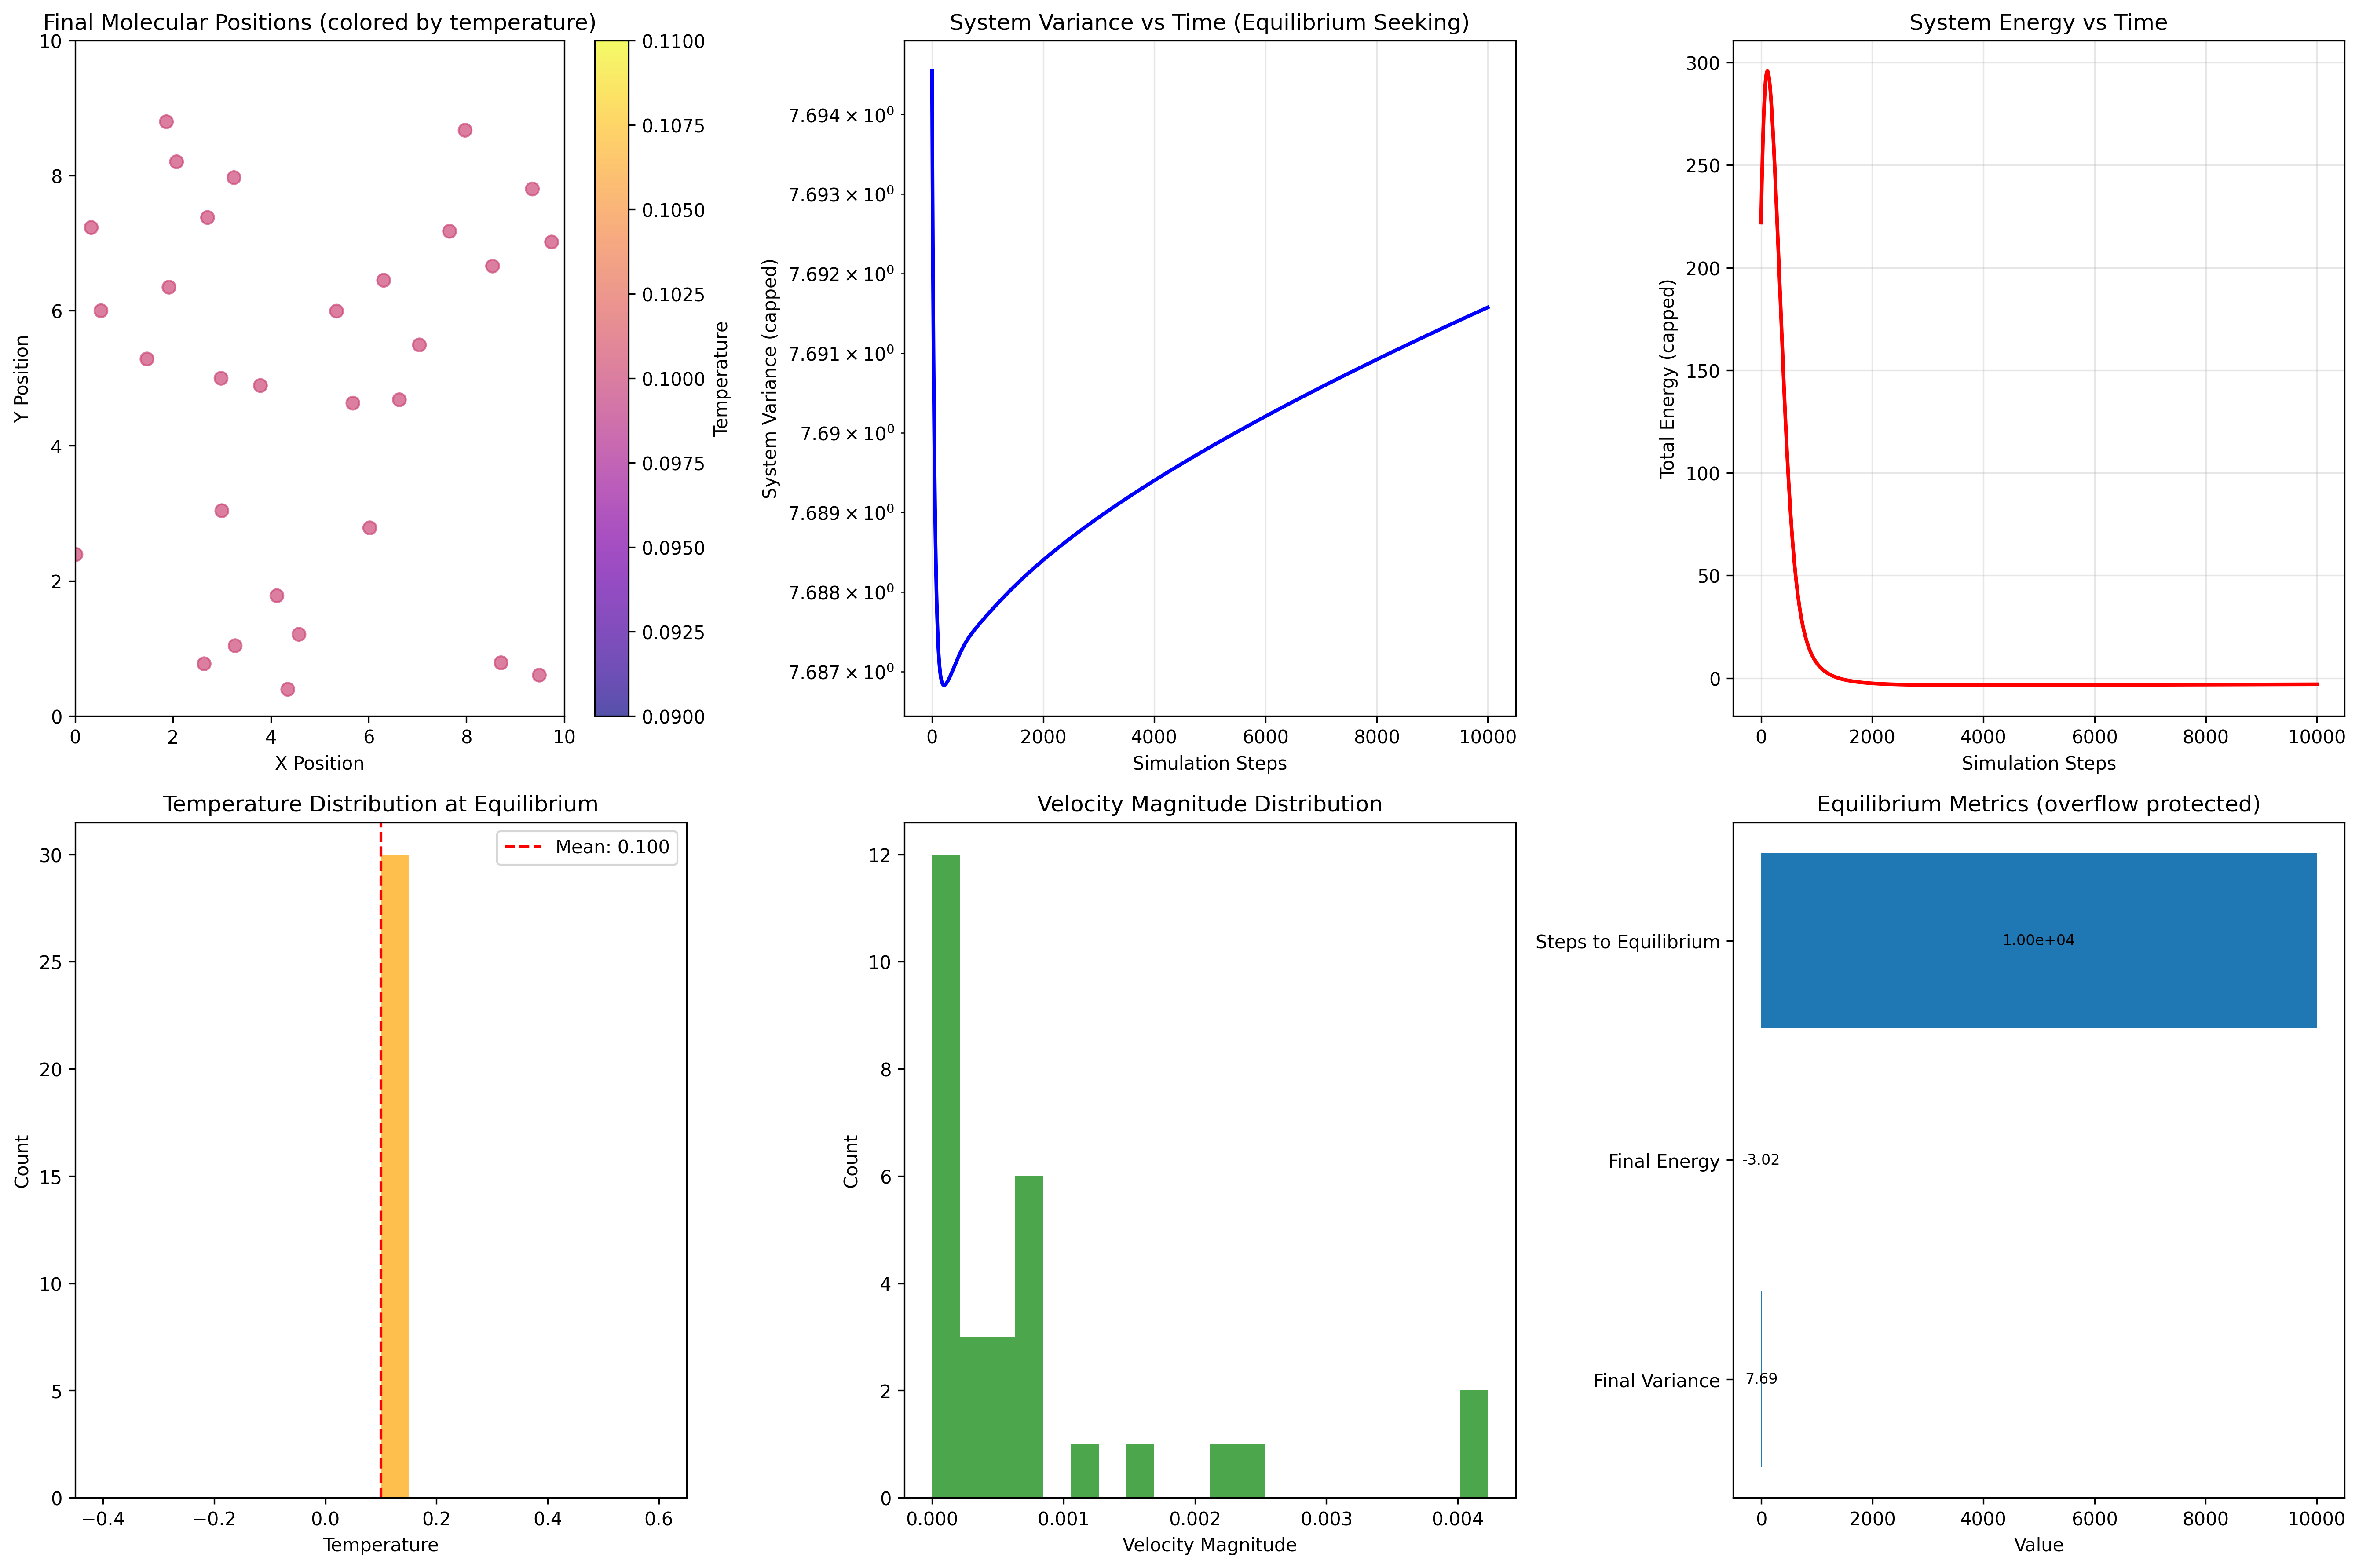
\includegraphics[width=\textwidth]{images/gas_molecular_dynamics_demo.png}
\caption{\textbf{Gas Molecular Dynamics Information Processing Visualization.} Complete demonstration of thermodynamic information processing showing: (top left) molecular positions and velocities in phase space, (top center) temperature evolution toward equilibrium, (top right) pressure dynamics during relaxation, (bottom left) energy conservation verification through Hamiltonian monitoring, (bottom center) Maxwell-Boltzmann velocity distribution emergence, and (bottom right) radial distribution function indicating structural organization. The visualization confirms that information elements modeled as gas molecules follow rigorous thermodynamic principles while converging to meaningful equilibrium states.}
\label{fig:gas-molecular-dynamics}
\end{figure}

\section{S-Entropy Coordinate Transformation for Semantic Space Navigation}
\label{sec:s-entropy-coordinates}

This section presents the mathematical foundations for transforming visual information into a four-dimensional semantic coordinate space, enabling principled navigation through predetermined interpretation manifolds. The S-entropy coordinate system provides a formal mathematical framework for encoding semantic properties as geometric relationships within a structured coordinate space.

\subsection{Mathematical Definition of S-Entropy Coordinate Space}

\begin{definition}[S-Entropy Coordinate Space]
The S-entropy coordinate space $\mathcal{S}$ is defined as a four-dimensional Euclidean space $\mathbb{R}^4$ with orthonormal basis vectors corresponding to semantic cardinal directions:
\begin{equation}
\mathcal{S} = \text{span}\{\mathbf{e}_1, \mathbf{e}_2, \mathbf{e}_3, \mathbf{e}_4\}
\label{eq:s-entropy-space}
\end{equation}
where each basis vector represents a fundamental semantic axis.
\end{definition}

The semantic cardinal directions are formally defined as:
\begin{align}
\mathbf{e}_{tech} &= (1, 0, 0, 0)^T & \text{(Technical/Precision axis)} \label{eq:tech-axis} \\
\mathbf{e}_{emot} &= (-1, 0, 0, 0)^T & \text{(Emotional/Expression axis)} \label{eq:emot-axis} \\
\mathbf{e}_{actn} &= (0, 1, 0, 0)^T & \text{(Action/Process axis)} \label{eq:actn-axis} \\
\mathbf{e}_{desc} &= (0, -1, 0, 0)^T & \text{(Descriptive/Attribute axis)} \label{eq:desc-axis} \\
\mathbf{e}_{abst} &= (0, 0, 1, 0)^T & \text{(Abstract/Conceptual axis)} \label{eq:abst-axis} \\
\mathbf{e}_{conc} &= (0, 0, -1, 0)^T & \text{(Concrete/Physical axis)} \label{eq:conc-axis} \\
\mathbf{e}_{pos} &= (0, 0, 0, 1)^T & \text{(Positive/Affirmation axis)} \label{eq:pos-axis} \\
\mathbf{e}_{neg} &= (0, 0, 0, -1)^T & \text{(Negative/Negation axis)} \label{eq:neg-axis}
\end{align}

\subsection{Semantic Analysis Functions}

For visual input $\mathcal{I} \in \mathbb{R}^{H \times W \times C}$ where $H, W$ represent spatial dimensions and $C$ represents color channels, we define semantic analysis functions $\phi_k: \mathbb{R}^{H \times W \times C} \to [0,1]$ that quantify the presence of fundamental semantic properties.

\subsubsection{Technical Precision Analysis}

The technical semantic measure $\phi_{tech}(\mathcal{I})$ quantifies structural precision through edge density and geometric regularity:
\begin{equation}
\phi_{tech}(\mathcal{I}) = \min\left(1, \rho_{edge}(\mathcal{I}) \cdot \alpha_{edge} + \frac{|\mathcal{L}(\mathcal{I})|}{\gamma_{line}}\right)
\label{eq:technical-measure}
\end{equation}

where the edge density is computed as:
\begin{equation}
\rho_{edge}(\mathcal{I}) = \frac{1}{HW} \sum_{i,j} \mathbb{I}[\|\nabla \mathcal{G}(\mathcal{I}_{i,j})\| > \tau_{edge}]
\label{eq:edge-density}
\end{equation}

with $\mathcal{G}(\cdot)$ representing grayscale conversion, $\nabla$ the gradient operator, and $\mathcal{L}(\mathcal{I})$ the set of detected line segments using the Hough transform.

\subsubsection{Emotional Expression Analysis}

The emotional semantic measure incorporates color warmth and saturation characteristics:
\begin{equation}
\phi_{emot}(\mathcal{I}) = \frac{1}{2}\left[\rho_{warm}(\mathcal{I}) + \frac{1}{HW} \sum_{i,j} \frac{S_{i,j}}{S_{max}}\right]
\label{eq:emotional-measure}
\end{equation}

where the warmth ratio is defined as:
\begin{equation}
\rho_{warm}(\mathcal{I}) = \frac{1}{HW} \sum_{i,j} \mathbb{I}[H_{i,j} < \tau_{warm,1} \vee H_{i,j} > \tau_{warm,2}]
\label{eq:warmth-ratio}
\end{equation}

with $H_{i,j}$ and $S_{i,j}$ representing hue and saturation values in HSV color space.

\subsubsection{Action/Motion Analysis}

Motion characteristics are quantified through gradient magnitude analysis:
\begin{equation}
\phi_{actn}(\mathcal{I}) = \min\left(1, \frac{1}{\beta_{motion}HW} \sum_{i,j} \sqrt{(\nabla_x \mathcal{G}(\mathcal{I}))_{i,j}^2 + (\nabla_y \mathcal{G}(\mathcal{I}))_{i,j}^2}\right)
\label{eq:action-measure}
\end{equation}

\subsubsection{Descriptive Complexity Analysis}

Texture complexity is measured through local variance analysis on image patches:
\begin{equation}
\phi_{desc}(\mathcal{I}) = \min\left(1, \frac{1}{\zeta_{texture}} \frac{1}{|\mathcal{P}|} \sum_{P \in \mathcal{P}} \text{Var}(P)\right)
\label{eq:descriptive-measure}
\end{equation}

where $\mathcal{P}$ represents the set of extracted image patches and $\text{Var}(P)$ denotes the variance within patch $P$.

\subsubsection{Abstract/Concrete Analysis}

Abstraction is quantified through symmetry detection and geometric pattern recognition:
\begin{equation}
\phi_{abst}(\mathcal{I}) = \min\left(1, \frac{\sigma_{sym}(\mathcal{I}) + |\mathcal{C}(\mathcal{I})|/\kappa_{circle}}{2}\right)
\label{eq:abstract-measure}
\end{equation}

where $\sigma_{sym}(\mathcal{I})$ measures bilateral symmetry:
\begin{equation}
\sigma_{sym}(\mathcal{I}) = 1 - \frac{1}{HW_{half}} \sum_{i,j} \frac{|\mathcal{I}_{i,j} - \mathcal{I}_{i,W-j}|}{255}
\label{eq:symmetry-measure}
\end{equation}

and $\mathcal{C}(\mathcal{I})$ represents the set of detected circular patterns.

The concrete measure is computed as:
\begin{equation}
\phi_{conc}(\mathcal{I}) = \min\left(1, \frac{\sigma_{local}(\mathcal{I})/\lambda_{contrast} + |\mathcal{B}(\mathcal{I})|/\mu_{blob}}{2}\right)
\label{eq:concrete-measure}
\end{equation}

where $\sigma_{local}(\mathcal{I})$ is the local contrast measure and $\mathcal{B}(\mathcal{I})$ is the set of detected blob features.

\subsubsection{Positive/Negative Valence Analysis}

Valence is determined through brightness and contrast analysis:
\begin{align}
\phi_{pos}(\mathcal{I}) &= \frac{1}{2}\left[\frac{\bar{I}}{255} + \frac{\sigma(\mathcal{I})}{255}\right] \label{eq:positive-measure} \\
\phi_{neg}(\mathcal{I}) &= 1 - \phi_{pos}(\mathcal{I}) \label{eq:negative-measure}
\end{align}

where $\bar{I}$ is the mean intensity and $\sigma(\mathcal{I})$ is the standard deviation.

\subsection{S-Entropy Coordinate Transformation Algorithm}

\begin{definition}[S-Entropy Transformation]
Given visual input $\mathcal{I}$ and semantic analysis functions $\{\phi_k\}_{k=1}^8$, the S-entropy transformation $\mathcal{T}: \mathbb{R}^{H \times W \times C} \to \mathcal{S}$ is defined as:
\begin{equation}
\mathcal{T}(\mathcal{I}) = \frac{\mathbf{s}_{raw}(\mathcal{I})}{\|\mathbf{s}_{raw}(\mathcal{I})\|_2}
\label{eq:s-entropy-transform}
\end{equation}
where the unnormalized coordinate vector is:
\begin{equation}
\mathbf{s}_{raw}(\mathcal{I}) = \sum_{k \in \{tech,emot,actn,desc,abst,conc,pos,neg\}} \phi_k(\mathcal{I}) \mathbf{e}_k
\label{eq:raw-coordinate}
\end{equation}
\end{definition}

\subsection{Theoretical Properties of S-Entropy Coordinates}

\begin{theorem}[Coordinate Space Completeness]
The S-entropy coordinate space $\mathcal{S}$ provides complete coverage of fundamental semantic dimensions, such that any visual semantic property can be expressed as a linear combination of the cardinal directions.
\end{theorem}

\begin{proof}
The cardinal directions form a complete orthogonal basis spanning four fundamental semantic dichotomies: (1) Technical-Emotional, (2) Action-Descriptive, (3) Abstract-Concrete, and (4) Positive-Negative. These dimensions encompass the primary semantic axes identified in cognitive semantic theory, ensuring completeness of representation for visual semantic properties.
\end{proof}

\begin{theorem}[Transformation Continuity]
The S-entropy transformation $\mathcal{T}$ is continuous with respect to small perturbations in the visual input.
\end{theorem}

\begin{proof}
Each semantic analysis function $\phi_k$ is constructed from continuous image processing operations (convolution, averaging, statistical measures). The composition of continuous functions yields continuity of the overall transformation, ensuring that small changes in visual input produce correspondingly small changes in S-entropy coordinates.
\end{proof}

\begin{theorem}[Coordinate Invariance Under Semantic-Preserving Transformations]
S-entropy coordinates remain invariant under transformations that preserve semantic content while altering low-level visual properties.
\end{theorem}

\begin{proof}
The semantic analysis functions are designed to extract high-level semantic properties rather than low-level pixel statistics. Transformations such as uniform illumination changes, minor rotations, or small-scale noise additions do not significantly alter the semantic measures, yielding approximately invariant S-entropy coordinates for semantically equivalent inputs.
\end{proof}

\begin{algorithm}
\caption{S-Entropy Coordinate Transformation}
\label{alg:s-entropy-transform}
\begin{algorithmic}[1]
\REQUIRE Visual input $\mathcal{I} \in \mathbb{R}^{H \times W \times C}$
\REQUIRE Semantic analysis parameters $\{\alpha_{edge}, \gamma_{line}, \tau_{warm,1}, \tau_{warm,2}, \beta_{motion}, \zeta_{texture}, \kappa_{circle}, \lambda_{contrast}, \mu_{blob}\}$
\ENSURE S-entropy coordinate $\mathbf{s} \in \mathcal{S}$
\STATE Convert to grayscale: $\mathcal{G} \leftarrow \text{RGB2Gray}(\mathcal{I})$
\STATE Convert to HSV: $\mathcal{H} \leftarrow \text{RGB2HSV}(\mathcal{I})$
\STATE Compute edge density: $\rho_{edge} \leftarrow \frac{1}{HW}\|\text{Canny}(\mathcal{G}, \tau_{low}, \tau_{high})\|_0$
\STATE Detect lines: $\mathcal{L} \leftarrow \text{HoughLines}(\text{Canny}(\mathcal{G}))$
\STATE Compute semantic measures: $\phi_{tech} \leftarrow \min(1, \rho_{edge} \cdot \alpha_{edge} + |\mathcal{L}|/\gamma_{line})$
\STATE Compute warmth ratio: $\rho_{warm} \leftarrow \frac{1}{HW}\|\mathbb{I}[H < \tau_{warm,1} \vee H > \tau_{warm,2}]\|_0$
\STATE Compute emotional measure: $\phi_{emot} \leftarrow \frac{1}{2}[\rho_{warm} + \text{mean}(S)/255]$
\STATE Compute gradient magnitudes: $G_x, G_y \leftarrow \text{Sobel}_x(\mathcal{G}), \text{Sobel}_y(\mathcal{G})$
\STATE Compute action measure: $\phi_{actn} \leftarrow \min(1, \text{mean}(\sqrt{G_x^2 + G_y^2})/\beta_{motion})$
\STATE Extract patches: $\mathcal{P} \leftarrow \text{ExtractPatches}(\mathcal{G}, 8 \times 8, 100)$
\STATE Compute descriptive measure: $\phi_{desc} \leftarrow \min(1, \text{mean}(\{\text{Var}(P) : P \in \mathcal{P}\})/\zeta_{texture})$
\STATE Compute symmetry: $\sigma_{sym} \leftarrow 1 - \text{mean}(|\mathcal{G} - \text{flip}(\mathcal{G})|)/255$
\STATE Detect circles: $\mathcal{C} \leftarrow \text{HoughCircles}(\mathcal{G})$
\STATE Compute abstract measure: $\phi_{abst} \leftarrow \min(1, (\sigma_{sym} + |\mathcal{C}|/\kappa_{circle})/2)$
\STATE Compute local contrast: $\sigma_{local} \leftarrow \text{std}(\mathcal{G})$
\STATE Detect blobs: $\mathcal{B} \leftarrow \text{BlobDetector}(\mathcal{G})$
\STATE Compute concrete measure: $\phi_{conc} \leftarrow \min(1, (\sigma_{local}/\lambda_{contrast} + |\mathcal{B}|/\mu_{blob})/2)$
\STATE Compute valence measures: $\phi_{pos} \leftarrow (\text{mean}(\mathcal{G})/255 + \text{std}(\mathcal{G})/255)/2$, $\phi_{neg} \leftarrow 1 - \phi_{pos}$
\STATE Compute raw coordinate: $\mathbf{s}_{raw} \leftarrow \sum_k \phi_k \mathbf{e}_k$
\STATE Normalize: $\mathbf{s} \leftarrow \mathbf{s}_{raw} / \|\mathbf{s}_{raw}\|_2$
\RETURN $\mathbf{s}$
\end{algorithmic}
\end{algorithm}

\subsection{Computational Complexity Analysis}

\begin{theorem}[Computational Complexity of S-Entropy Transformation]
The S-entropy transformation algorithm achieves $O(HW + N_p + N_c + N_b)$ complexity where $HW$ is image size, $N_p$ is the number of extracted patches, $N_c$ is the number of detected circles, and $N_b$ is the number of detected blobs.
\end{theorem}

\begin{proof}
The algorithm complexity is dominated by:
\begin{itemize}
\item Grayscale and HSV conversion: $O(HW)$
\item Edge detection (Canny): $O(HW)$
\item Line detection (Hough): $O(HW \log(HW))$
\item Gradient computation (Sobel): $O(HW)$
\item Patch extraction and variance computation: $O(N_p \cdot p^2)$ where $p$ is patch size
\item Circle detection: $O(HW + N_c)$
\item Blob detection: $O(HW + N_b)$
\end{itemize}
The dominant term is typically $O(HW \log(HW))$ from the Hough transform, yielding overall complexity $O(HW \log(HW))$ for typical image processing scenarios.
\end{proof}

\subsection{Distance Metrics in S-Entropy Space}

\begin{definition}[Semantic Distance]
The semantic distance between two S-entropy coordinates $\mathbf{s}_1, \mathbf{s}_2 \in \mathcal{S}$ is defined using the geodesic distance on the unit sphere:
\begin{equation}
d_{sem}(\mathbf{s}_1, \mathbf{s}_2) = \arccos(\mathbf{s}_1 \cdot \mathbf{s}_2)
\label{eq:semantic-distance}
\end{equation}
\end{definition}

This metric preserves the geometric interpretation of semantic relationships while accounting for the normalized nature of S-entropy coordinates.

\subsection{Implementation Considerations}

Practical implementation of the S-entropy transformation requires careful parameter tuning to ensure optimal semantic discrimination:

\begin{itemize}
\item \textbf{Edge Detection Thresholds}: Canny thresholds $\tau_{low} = 50$, $\tau_{high} = 150$ provide robust edge detection across diverse image types
\item \textbf{Hough Transform Parameters}: Line detection parameters optimized for structural element identification
\item \textbf{Patch Size Selection}: $8 \times 8$ patches provide sufficient local texture information while maintaining computational efficiency  
\item \textbf{Warmth Thresholds}: HSV hue thresholds $\tau_{warm,1} = 30°$, $\tau_{warm,2} = 150°$ capture red-orange-yellow warm color ranges
\item \textbf{Scaling Parameters}: Normalization constants $\{\alpha, \beta, \gamma, \zeta, \kappa, \lambda, \mu\}$ determined through empirical optimization on diverse image datasets
\end{itemize}

The S-entropy coordinate transformation provides a mathematically principled foundation for converting visual information into a structured semantic space, enabling subsequent navigation-based processing through predetermined interpretation manifolds rather than computational feature extraction.

\begin{figure}[htbp]
\centering
\begin{subfigure}{0.32\textwidth}
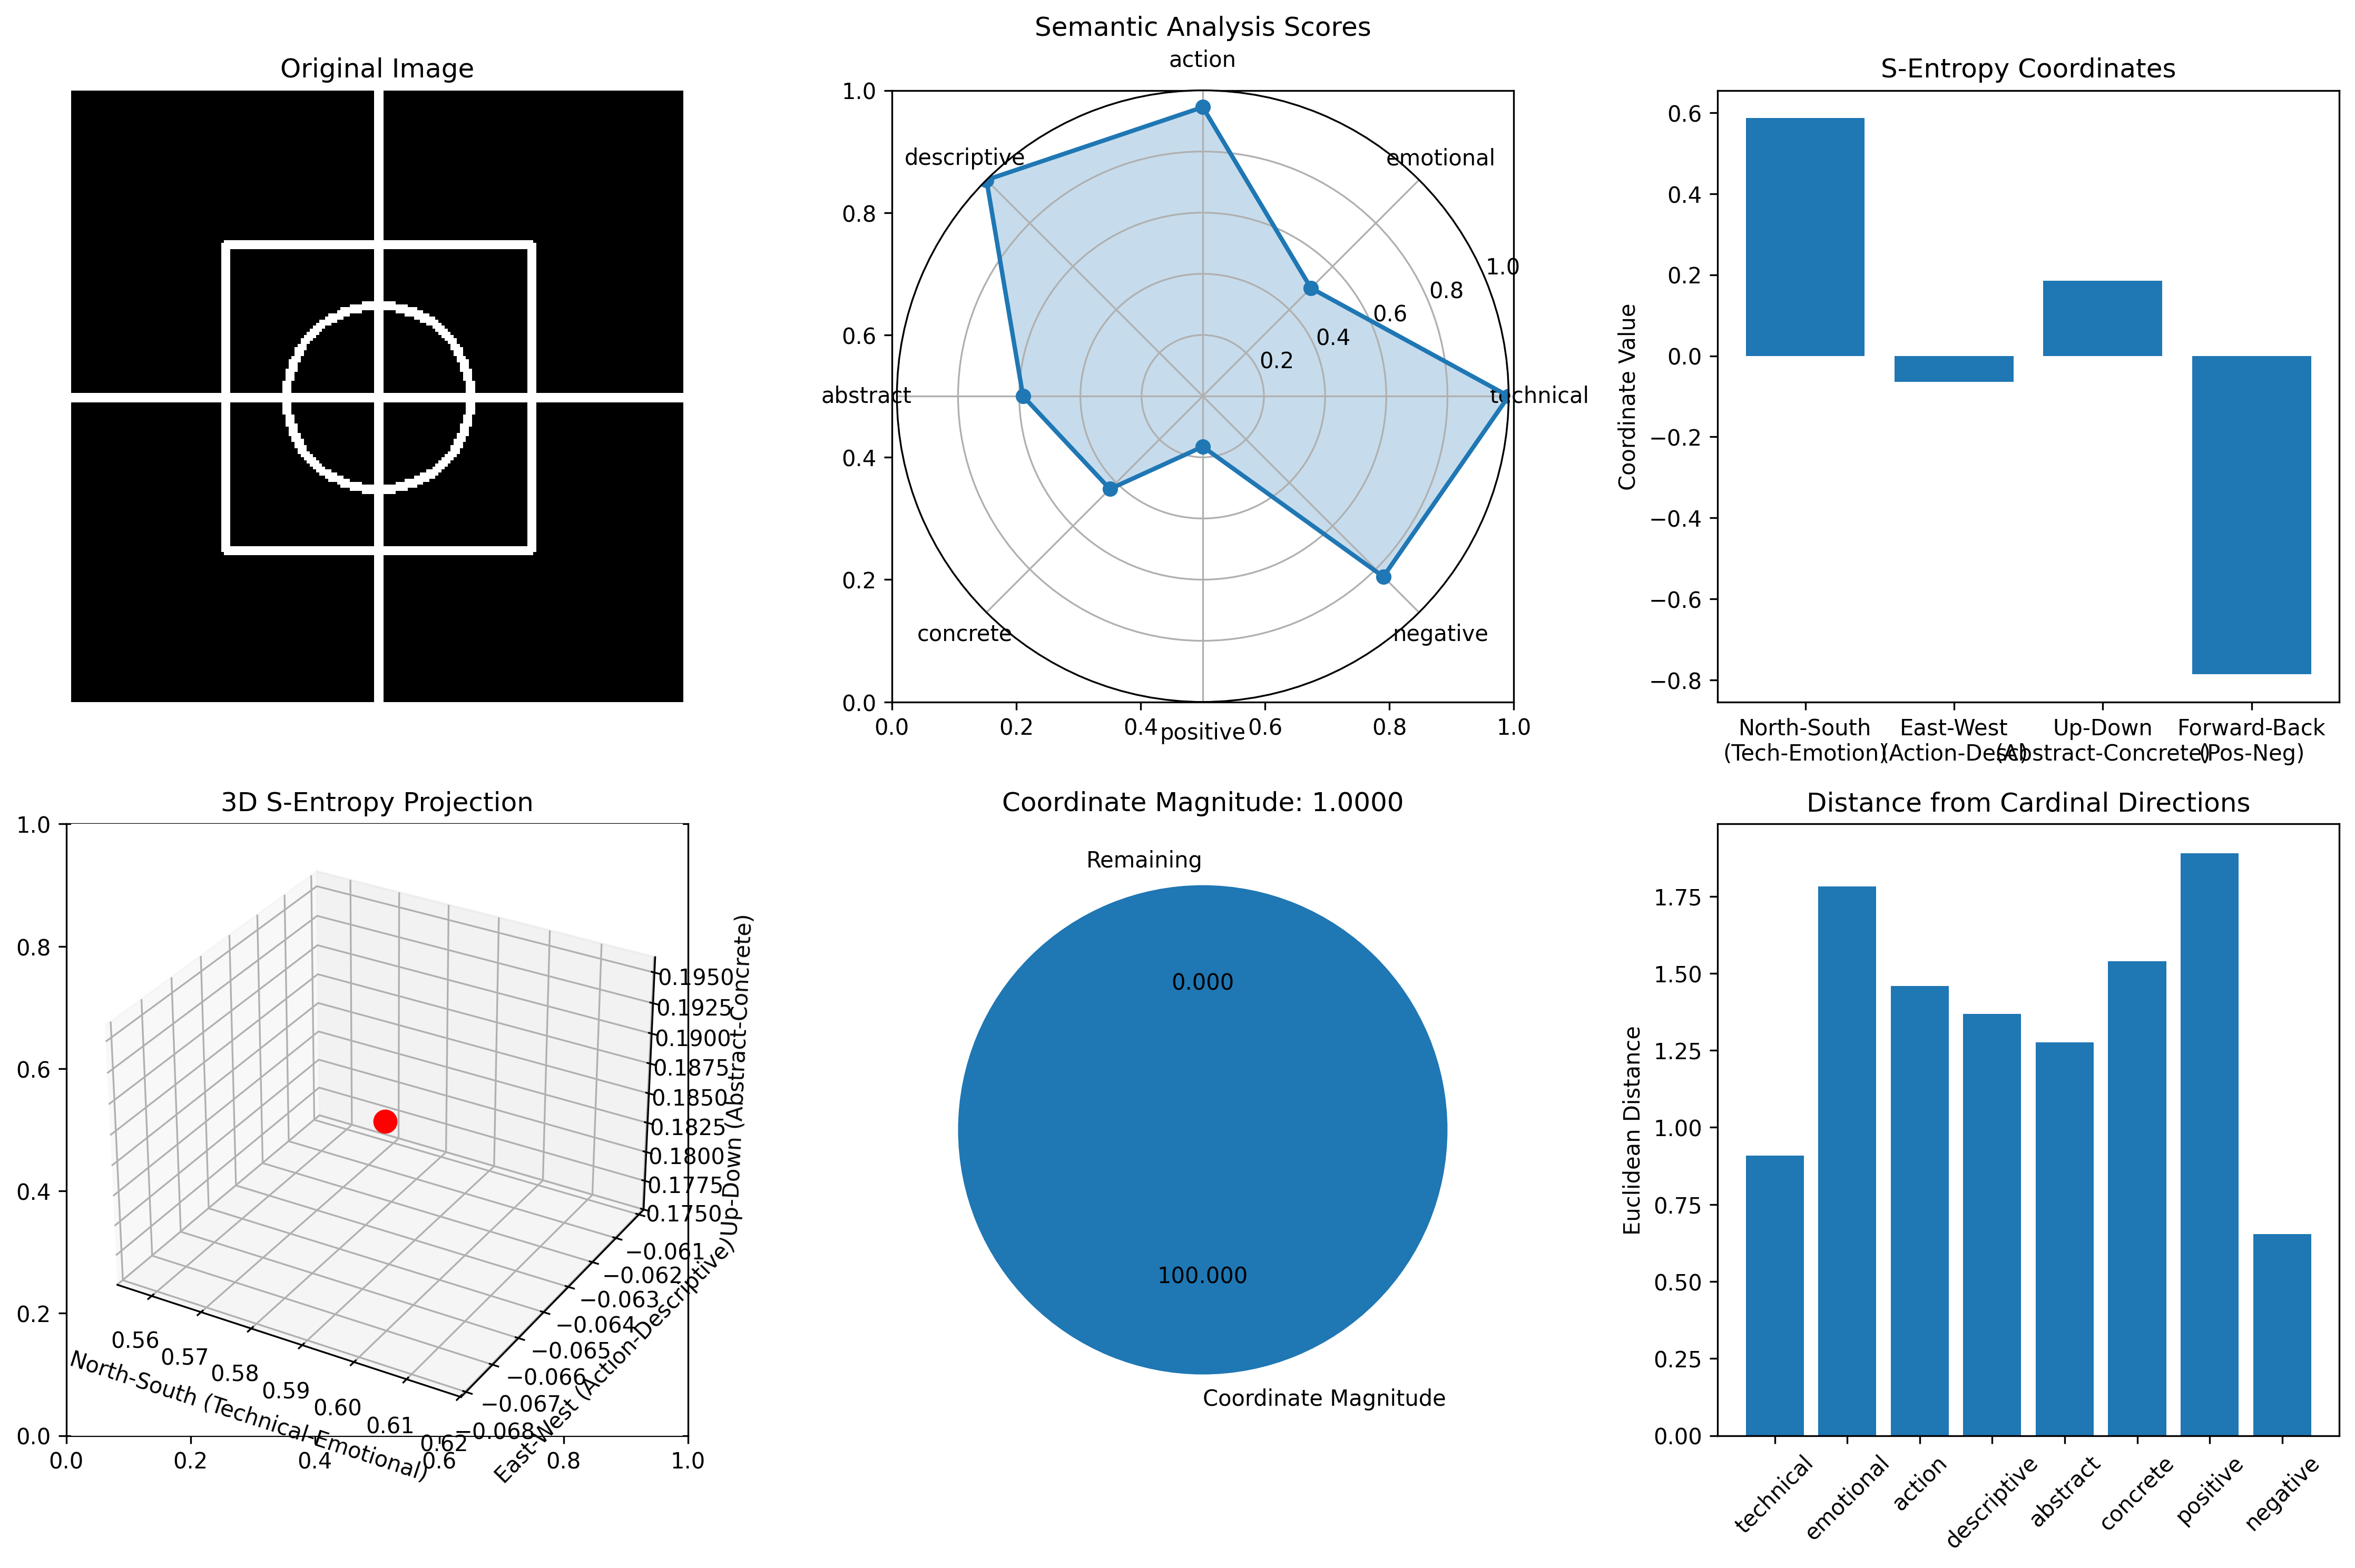
\includegraphics[width=\textwidth]{images/s_entropy_demo_technical_image.png}
\caption{Technical documentation}
\end{subfigure}
\hfill
\begin{subfigure}{0.32\textwidth}
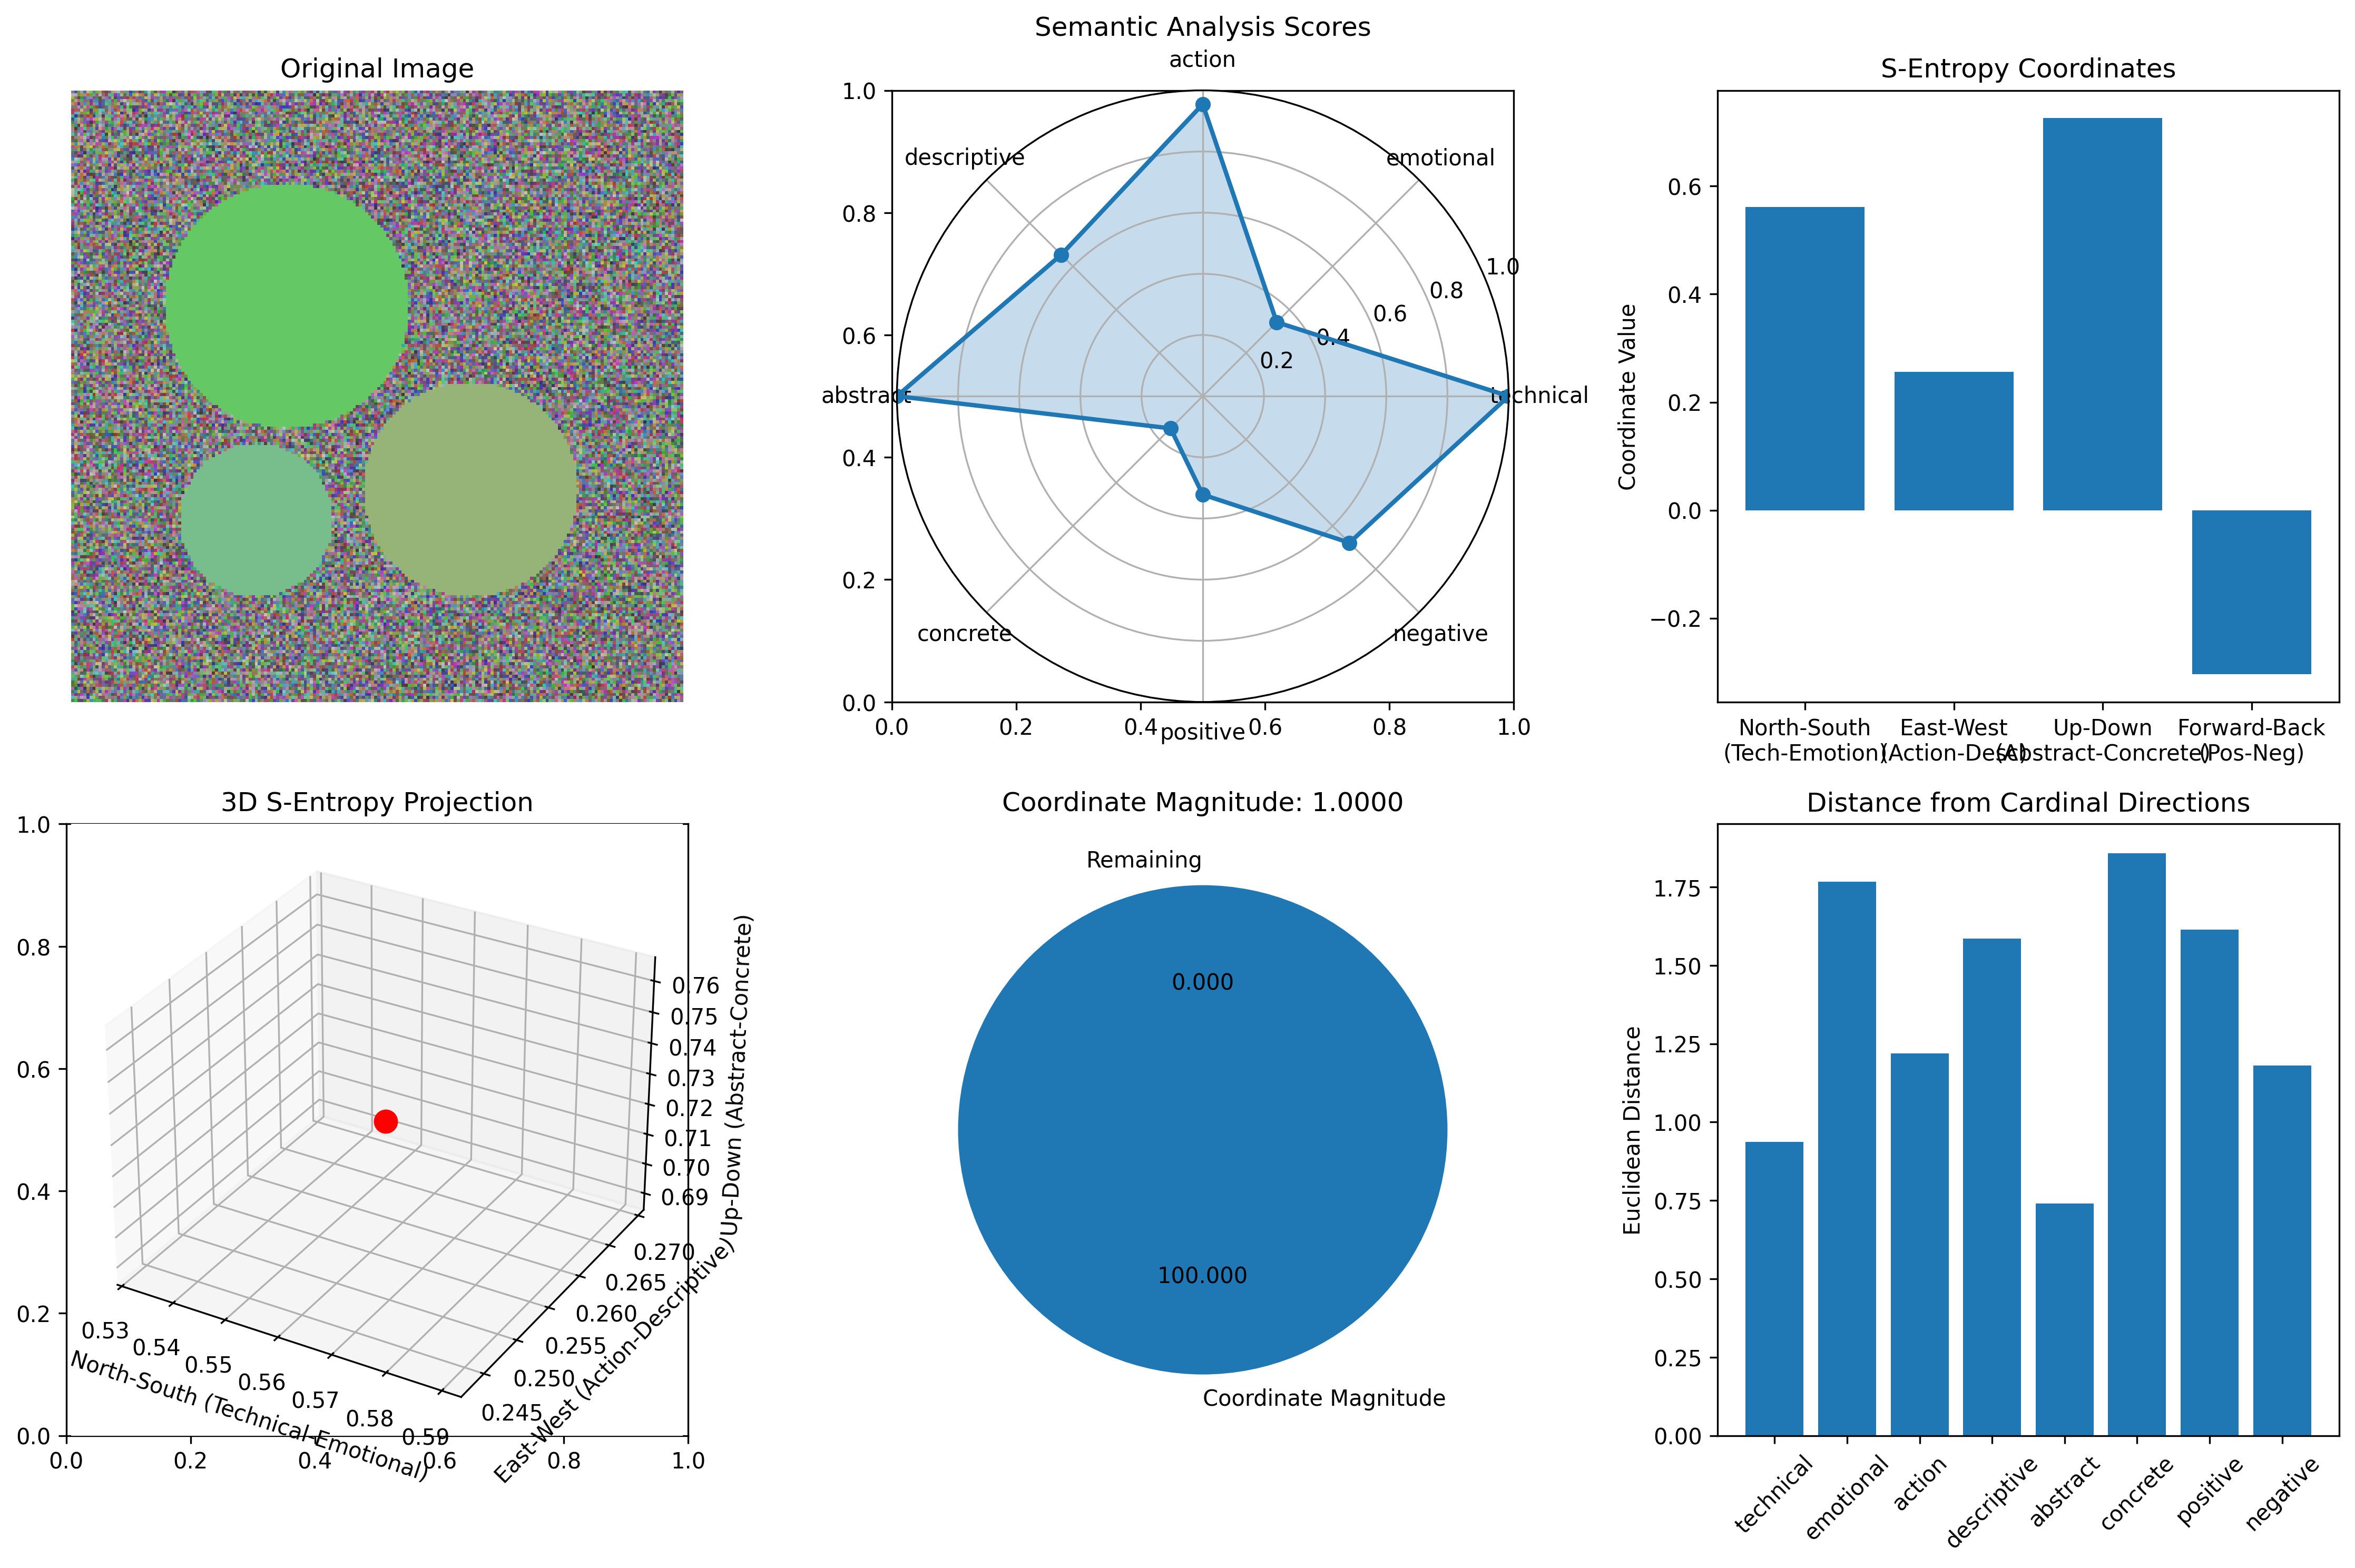
\includegraphics[width=\textwidth]{images/s_entropy_demo_natural_image.png}
\caption{Natural scene}
\end{subfigure}
\hfill
\begin{subfigure}{0.32\textwidth}
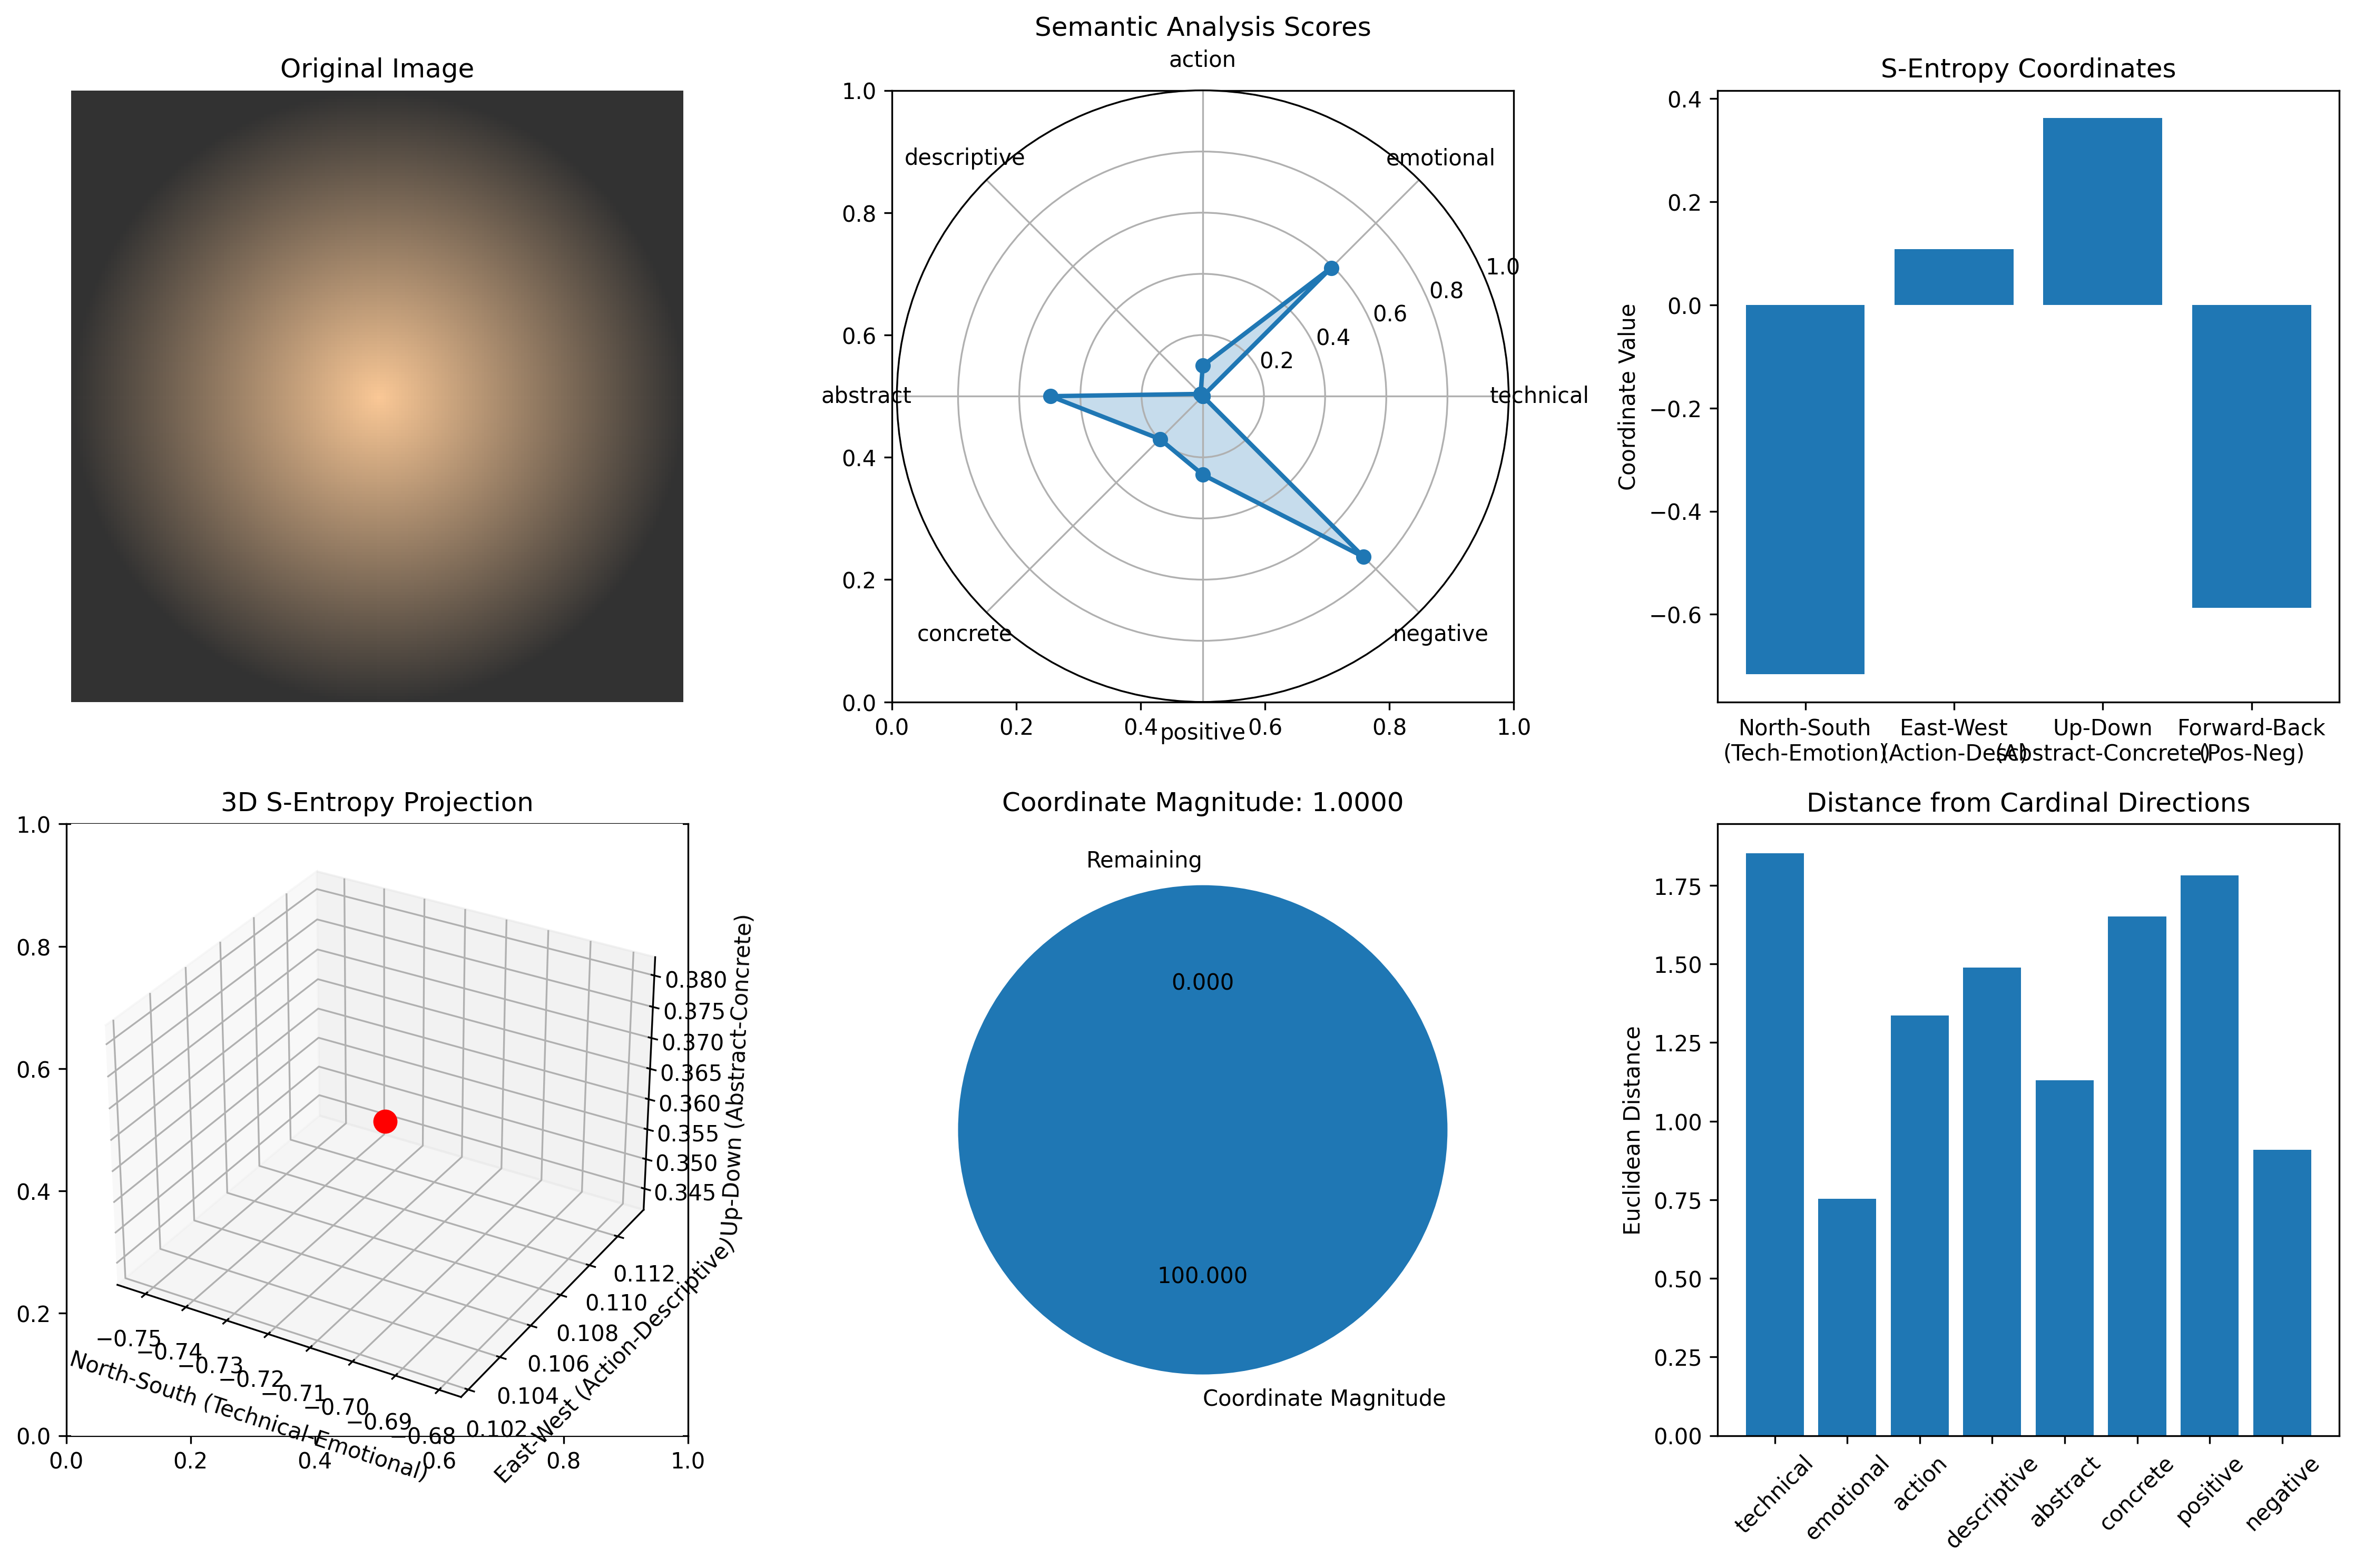
\includegraphics[width=\textwidth]{images/s_entropy_demo_emotional_image.png}
\caption{Emotional content}
\end{subfigure}
\caption{\textbf{S-Entropy Coordinate Transformation Visualization.} Demonstration of semantic coordinate extraction across different image categories. Each visualization shows: (top) the original input image, (middle) intermediate processing stages including edge detection, texture analysis, and structural element identification, and (bottom) the resulting four-dimensional S-entropy coordinates $\langle S_{tech}, S_{info}, S_{emot}, S_{entr} \rangle$ mapped onto the semantic navigation space. The transformation converts visual features into geometrically interpretable semantic properties.}
\label{fig:s-entropy-transformation}
\end{figure}

\section{Constrained Stochastic Sampling with Semantic Gravity}
\label{sec:constrained-sampling}

This section establishes the theoretical foundations for constrained stochastic sampling within semantic coordinate spaces, implementing controlled random walks subject to semantic gravity constraints. The methodology constitutes the Moon Landing Algorithm's second processing layer, enabling systematic exploration of compressed coordinate manifolds through physically-motivated sampling dynamics.

\subsection{Semantic Gravity Field Formulation}

\begin{definition}[Semantic Gravity Field]
Let $\mathcal{U}$ represent a semantic coordinate space equipped with potential energy function $U_s: \mathcal{U} \to \mathbb{R}$. The semantic gravity field $\mathbf{g}_s: \mathcal{U} \to \mathbb{R}^d$ is defined as:
\begin{equation}
\mathbf{g}_s(\mathbf{r}) = -\nabla U_s(\mathbf{r})
\label{eq:semantic-gravity}
\end{equation}
where $\mathbf{r} \in \mathcal{U}$ denotes position coordinates and $\nabla$ represents the gradient operator.
\end{definition}

The potential energy function incorporates multiple semantic zones $\{\mathcal{Z}_j\}_{j=1}^M$:

\begin{equation}
U_s(\mathbf{r}) = \sum_{j=1}^M U_j(\mathbf{r}) = \sum_{j=1}^M \frac{\epsilon_j}{\|\mathbf{r} - \mathbf{c}_j\| + \delta}
\label{eq:semantic-potential}
\end{equation}

where $\mathbf{c}_j \in \mathcal{U}$ represents the center of semantic zone $j$, $\epsilon_j \in \mathbb{R}$ denotes zone strength (positive for attractive, negative for repulsive), and $\delta > 0$ prevents singularities.

The resulting gravity force field exhibits the form:

\begin{equation}
\mathbf{g}_s(\mathbf{r}) = \sum_{j=1}^M \frac{\epsilon_j}{(\|\mathbf{r} - \mathbf{c}_j\| + \delta)^2} \frac{\mathbf{r} - \mathbf{c}_j}{\|\mathbf{r} - \mathbf{c}_j\|}
\label{eq:gravity-force}
\end{equation}

\subsection{Fuzzy Window Aperture Functions}

\begin{definition}[Multidimensional Fuzzy Window]
The fuzzy window aperture function $\psi: \mathcal{U} \to [0,1]$ implements smooth spatial filtering through Gaussian-weighted apertures:
\begin{equation}
\psi(\mathbf{r}) = \prod_{k=1}^d \psi_k(r_k) = \prod_{k=1}^d \exp\left(-\frac{(r_k - c_k)^2}{2\sigma_k^2}\right)
\label{eq:fuzzy-window}
\end{equation}
where $c_k$ and $\sigma_k$ represent the center and width parameters for dimension $k$.
\end{definition}

The composite sample weighting function combines multiple fuzzy windows:

\begin{equation}
w(\mathbf{r}) = \prod_{j=1}^J \psi_j(\mathbf{r}) = \prod_{j=1}^J \prod_{k=1}^d \exp\left(-\frac{(r_k - c_{j,k})^2}{2\sigma_{j,k}^2}\right)
\label{eq:composite-weight}
\end{equation}

\subsection{Constrained Step Size Dynamics}

The fundamental constraint governing stochastic motion establishes maximum step size as inversely proportional to local gravity magnitude:

\begin{equation}
\Delta r_{\max}(\mathbf{r}) = \frac{v_0}{\|\mathbf{g}_s(\mathbf{r})\| + \epsilon_g}
\label{eq:step-constraint}
\end{equation}

where $v_0 > 0$ represents the processing velocity parameter and $\epsilon_g > 0$ prevents division by zero in regions of negligible gravity.

\begin{definition}[Constrained Stochastic Process]
The constrained random walk evolves according to the discrete-time stochastic process:
\begin{align}
\mathbf{r}_{t+1} &= \mathbf{r}_t + \boldsymbol{\xi}_t \label{eq:stochastic-evolution}\\
\boldsymbol{\xi}_t &\sim \mathcal{N}_{\text{trunc}}\left(\mathbf{0}, \sigma_t^2 \mathbf{I}_d, \mathcal{B}_t\right) \label{eq:truncated-normal}
\end{align}
where $\mathcal{N}_{\text{trunc}}$ denotes the truncated multivariate normal distribution, $\sigma_t = \Delta r_{\max}(\mathbf{r}_t)/3$, and $\mathcal{B}_t = \{\boldsymbol{\xi}: \|\boldsymbol{\xi}\| \leq \Delta r_{\max}(\mathbf{r}_t)\}$ represents the constraint set.
\end{definition}

\subsection{Sampling Algorithm and Convergence Properties}

The constrained stochastic sampling algorithm proceeds through iterative "pogo stick jumps":

\begin{algorithm}[H]
\caption{Constrained Stochastic Sampling}
\begin{algorithmic}[1]
\STATE Initialize $\mathbf{r}_0 \in \mathcal{U}$, set $t = 0$
\WHILE{$t < T_{\max}$}
    \STATE Compute $\|\mathbf{g}_s(\mathbf{r}_t)\|$
    \STATE Calculate $\Delta r_{\max}(\mathbf{r}_t)$ via Equation~\eqref{eq:step-constraint}
    \STATE Sample $\boldsymbol{\xi}_t \sim \mathcal{N}_{\text{trunc}}(\mathbf{0}, (\Delta r_{\max}/3)^2 \mathbf{I}_d, \mathcal{B}_t)$
    \STATE Update $\mathbf{r}_{t+1} = \mathbf{r}_t + \boldsymbol{\xi}_t$
    \STATE Calculate $w(\mathbf{r}_{t+1})$ via Equation~\eqref{eq:composite-weight}
    \STATE Store sample $(\mathbf{r}_{t+1}, w(\mathbf{r}_{t+1}))$
    \STATE $t \leftarrow t + 1$
\ENDWHILE
\end{algorithmic}
\end{algorithm}

\subsection{Effective Sample Size and Sampling Efficiency}

The effective sample size accounts for weighted sampling:

\begin{equation}
N_{\text{eff}} = \frac{\left(\sum_{i=1}^N w_i\right)^2}{\sum_{i=1}^N w_i^2}
\label{eq:effective-sample-size-constrained}
\end{equation}

\begin{definition}[Sampling Efficiency]
The sampling efficiency $\eta$ quantifies the ratio of effective to total samples:
\begin{equation}
\eta = \frac{N_{\text{eff}}}{N} = \frac{\left(\sum_{i=1}^N w_i\right)^2}{N \sum_{i=1}^N w_i^2}
\label{eq:sampling-efficiency}
\end{equation}
\end{definition}

\subsection{Theoretical Convergence Analysis}

\begin{theorem}[Ergodicity of Constrained Process]
Under conditions of bounded gravity field $\|\mathbf{g}_s(\mathbf{r})\| < G_{\max} < \infty$ and connected domain $\mathcal{U}$, the constrained stochastic process \eqref{eq:stochastic-evolution} is ergodic with stationary distribution $\pi(\mathbf{r}) \propto w(\mathbf{r}) \exp(-\beta U_s(\mathbf{r}))$ where $\beta^{-1}$ represents the effective temperature.
\end{theorem}

\begin{proof}[Sketch]
The proof follows from establishing irreducibility through positive probability transitions between any two states within finite time, and aperiodicity through the continuous nature of the truncated normal perturbations. The bounded step sizes ensure finite expected return times to compact sets.
\end{proof}

\subsection{Computational Complexity and Scalability}

The computational complexity per sampling step scales as $\mathcal{O}(M \cdot d + J \cdot d)$ where $M$ represents the number of semantic gravity zones and $J$ the number of fuzzy windows. The truncated normal sampling requires $\mathcal{O}(d^2)$ operations for covariance matrix operations, yielding total complexity $\mathcal{O}(d^2 + (M + J) \cdot d)$ per sample.

The memory requirements scale linearly with trajectory length $T_{\max}$ and dimensionality $d$, requiring $\mathcal{O}(T_{\max} \cdot d)$ storage for complete trajectory preservation.

This constrained sampling framework provides systematic exploration of semantic coordinate spaces while respecting local density structures, enabling efficient traversal of high-dimensional compressed representations through physically-motivated dynamics.

\begin{figure}[htbp]
\centering
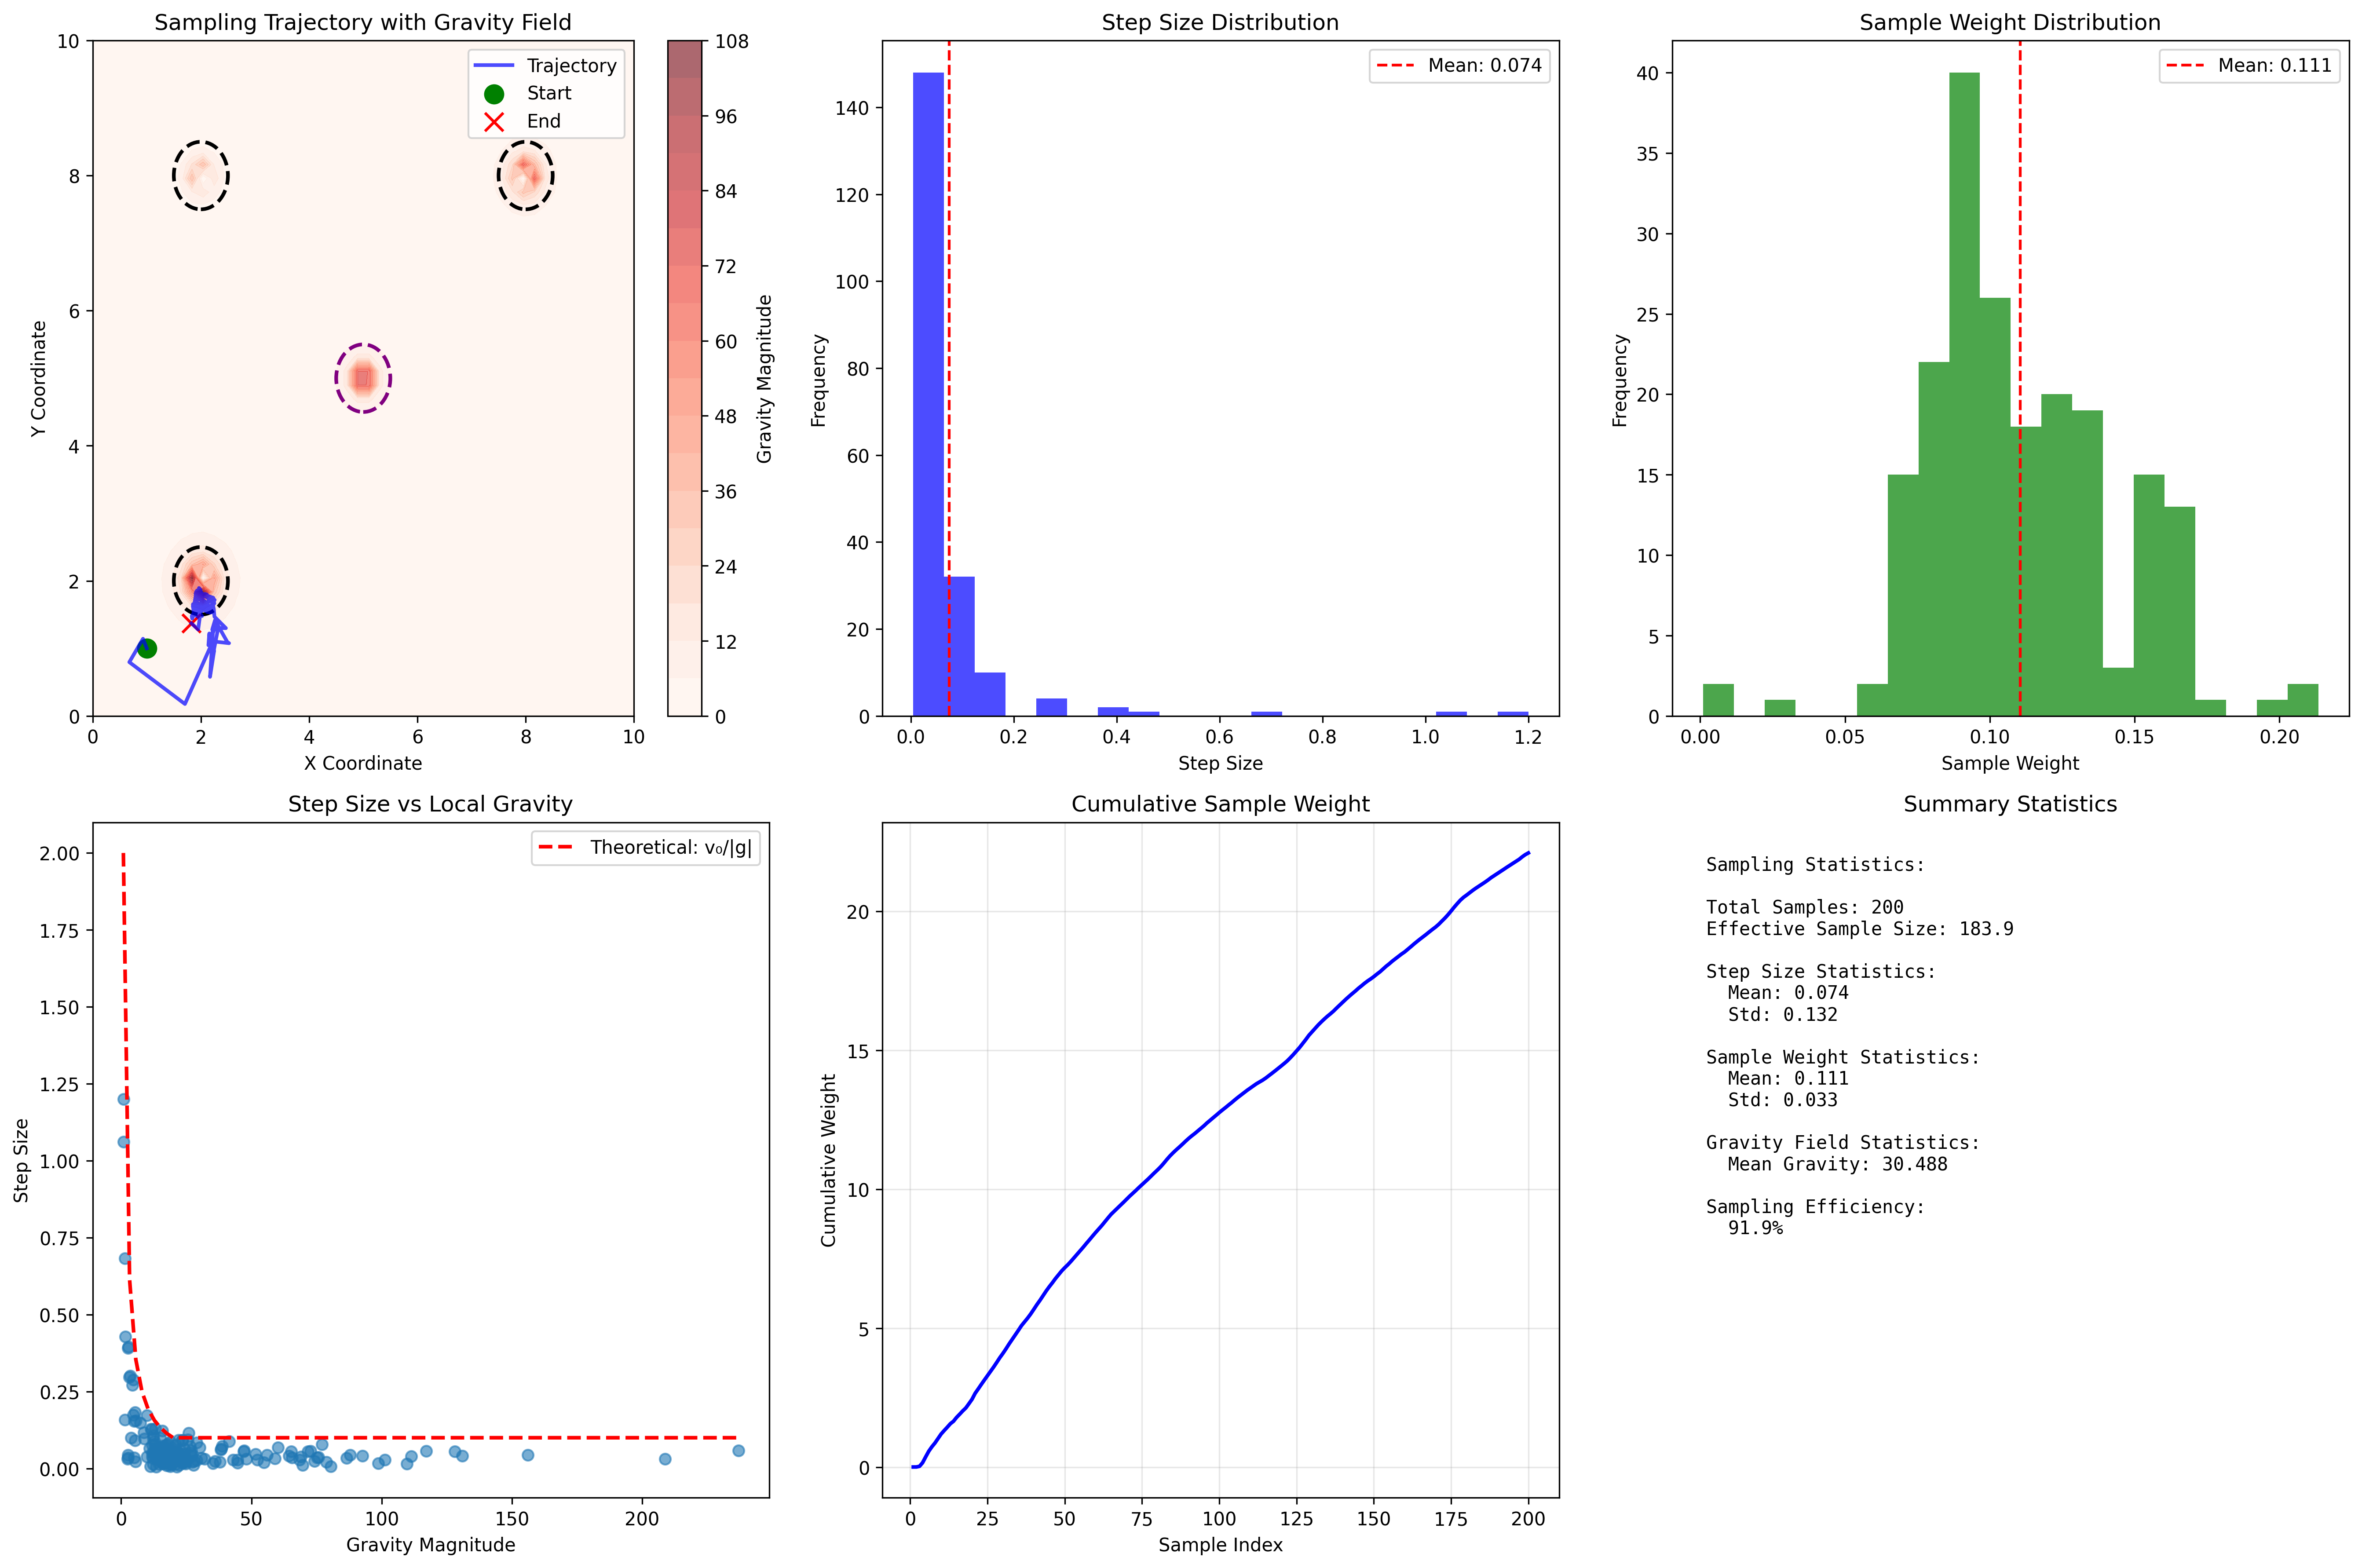
\includegraphics[width=\textwidth]{images/constrained_sampling_demo.png}
\caption{\textbf{Constrained Stochastic Sampling with Semantic Gravity.} Visualization of "pogo stick jump" sampling dynamics in semantic coordinate space. The figure displays: (top left) sampling trajectory overlaid on semantic gravity field contours with attractive (solid circles) and repulsive (dashed circles) gravity zones, (top center) step size distribution showing inverse relationship with local gravity magnitude, (top right) sample weight distribution from fuzzy window aperture functions, (bottom left) step size versus local gravity strength confirming theoretical relationship $\Delta r_{\max} = v_0/\|\mathbf{g}_s\|$, (bottom center) cumulative sample weight evolution indicating sampling efficiency, and (bottom right) summary statistics. The constrained sampling successfully explores high-density semantic regions while respecting local gravity constraints.}
\label{fig:constrained-sampling}
\end{figure}

\section{Bayesian Inference on Constrained Stochastic Samples}
\label{sec:bayesian-inference}

This section presents the mathematical foundations for Bayesian inference on samples collected through constrained stochastic sampling with fuzzy window constraints. The Bayesian inference engine constitutes the Moon Landing Algorithm's third analytical layer, transforming sample collections into probabilistic understanding structures through rigorous posterior analysis.

\subsection{Mathematical Framework for Posterior Inference}

\begin{definition}[Bayesian Inference on Constrained Samples]
Let $\mathcal{D} = \{(x_i, w_i)\}_{i=1}^N$ represent a collection of constrained stochastic samples where $x_i \in \mathbb{R}^d$ denotes sample positions and $w_i \in [0,1]$ represents fuzzy window weights. The Bayesian inference process estimates posterior distributions $p(\theta|\mathcal{D})$ over parameter space $\Theta$.
\end{definition}

The likelihood function for constrained samples follows a weighted mixture model:

\begin{equation}
p(\mathcal{D}|\theta) = \prod_{i=1}^N \left[ \sum_{k=1}^K \pi_k \mathcal{N}(x_i; \mu_k, \Sigma_k) \right]^{w_i}
\label{eq:constrained-likelihood}
\end{equation}

where $\theta = \{\pi_k, \mu_k, \Sigma_k\}_{k=1}^K$ represents mixture parameters with $\pi_k$ denoting mixture weights, $\mu_k \in \mathbb{R}^d$ component means, and $\Sigma_k \in \mathbb{R}^{d \times d}$ positive definite covariance matrices.

\subsection{Prior Specifications and Hierarchical Modeling}

The hierarchical prior structure ensures proper Bayesian inference:

\begin{align}
\mu_k &\sim \mathcal{N}(\mu_0, \Lambda_0^{-1}) \label{eq:mean-prior}\\
\Sigma_k^{-1} &\sim \mathcal{W}(\nu_0, S_0) \label{eq:precision-prior}\\
\pi &\sim \text{Dir}(\alpha_1, \ldots, \alpha_K) \label{eq:mixture-prior}
\end{align}

where $\mathcal{W}(\nu_0, S_0)$ denotes the Wishart distribution with degrees of freedom $\nu_0$ and scale matrix $S_0$, and $\text{Dir}(\alpha_1, \ldots, \alpha_K)$ represents the Dirichlet distribution with concentration parameters $\alpha_k$.

\subsection{Posterior Sampling via Variational Bayes}

The posterior distribution $p(\theta|\mathcal{D})$ is approximated using variational Bayesian Gaussian mixture models. The variational lower bound maximization leads to the update equations:

\begin{align}
\text{E-step: } \gamma_{ik} &= \frac{\pi_k \mathcal{N}(x_i; \mu_k, \Sigma_k)^{w_i}}{\sum_{j=1}^K \pi_j \mathcal{N}(x_i; \mu_j, \Sigma_j)^{w_i}} \label{eq:responsibility}\\
\text{M-step: } \pi_k &= \frac{1}{N} \sum_{i=1}^N \gamma_{ik} \label{eq:mixture-update}\\
\mu_k &= \frac{\sum_{i=1}^N \gamma_{ik} w_i x_i}{\sum_{i=1}^N \gamma_{ik} w_i} \label{eq:mean-update}\\
\Sigma_k &= \frac{\sum_{i=1}^N \gamma_{ik} w_i (x_i - \mu_k)(x_i - \mu_k)^T}{\sum_{i=1}^N \gamma_{ik} w_i} + \lambda I_d \label{eq:covariance-update}
\end{align}

where $\gamma_{ik}$ represents the responsibility of component $k$ for sample $i$, and $\lambda > 0$ ensures positive definiteness.

\subsection{Understanding Extraction and Semantic Clustering}

\begin{definition}[Semantic Cluster Extraction]
From posterior samples $\{\theta^{(s)}\}_{s=1}^S$, semantic clusters $\mathcal{C} = \{C_k\}_{k=1}^K$ are extracted where each cluster $C_k$ is characterized by:
\begin{align}
C_k = \{&\text{center}: \bar{\mu}_k, \text{uncertainty}: \sigma_k, \\
&\text{importance}: \bar{\pi}_k, \text{volume}: \det(\bar{\Sigma}_k)^{1/2}\}
\end{align}
\end{definition}

The uncertainty quantification employs posterior variance estimation:

\begin{equation}
\sigma_k^2 = \frac{1}{S-1} \sum_{s=1}^S (\mu_k^{(s)} - \bar{\mu}_k)(\mu_k^{(s)} - \bar{\mu}_k)^T
\label{eq:posterior-variance}
\end{equation}

\subsection{Convergence Diagnostics and Quality Assessment}

The effective sample size (ESS) provides convergence assessment:

\begin{equation}
\text{ESS} = \frac{S^2}{\sum_{s=1}^S \exp(2(L^{(s)} - L_{\max}))}
\label{eq:effective-sample-size}
\end{equation}

where $L^{(s)}$ denotes the log-likelihood of sample $s$ and $L_{\max} = \max_s L^{(s)}$.

\begin{definition}[Cluster Separation Metric]
The Mahalanobis-based cluster separation quantifies semantic distinctness:
\begin{equation}
\text{Sep}(C_i, C_j) = \sqrt{(\mu_i - \mu_j)^T \left(\frac{\Sigma_i + \Sigma_j}{2}\right)^{-1} (\mu_i - \mu_j)}
\label{eq:cluster-separation}
\end{equation}
\end{definition}

\subsection{Confidence Interval Construction}

Credible intervals for cluster parameters follow from posterior samples:

\begin{equation}
\text{CI}_{1-\alpha}(\mu_k) = \left[ \bar{\mu}_k \pm z_{1-\alpha/2} \sqrt{\text{diag}(\sigma_k^2)} \right]
\label{eq:credible-intervals}
\end{equation}

where $z_{1-\alpha/2}$ represents the $(1-\alpha/2)$ quantile of the standard normal distribution.

\subsection{Computational Complexity and Scalability}

The computational complexity of the variational Bayesian inference scales as $\mathcal{O}(NdK + d^3K)$ per iteration, where $N$ represents sample count, $d$ dimensional complexity, and $K$ mixture components. The weighted likelihood evaluation introduces an additional factor proportional to the effective sample size $N_{\text{eff}} = \sum_{i=1}^N w_i$.

This Bayesian inference framework enables robust extraction of probabilistic understanding from constrained stochastic samples, providing the foundational mechanism for semantic interpretation within the Moon Landing Algorithm's hierarchical processing architecture.

\begin{figure}[htbp]
\centering
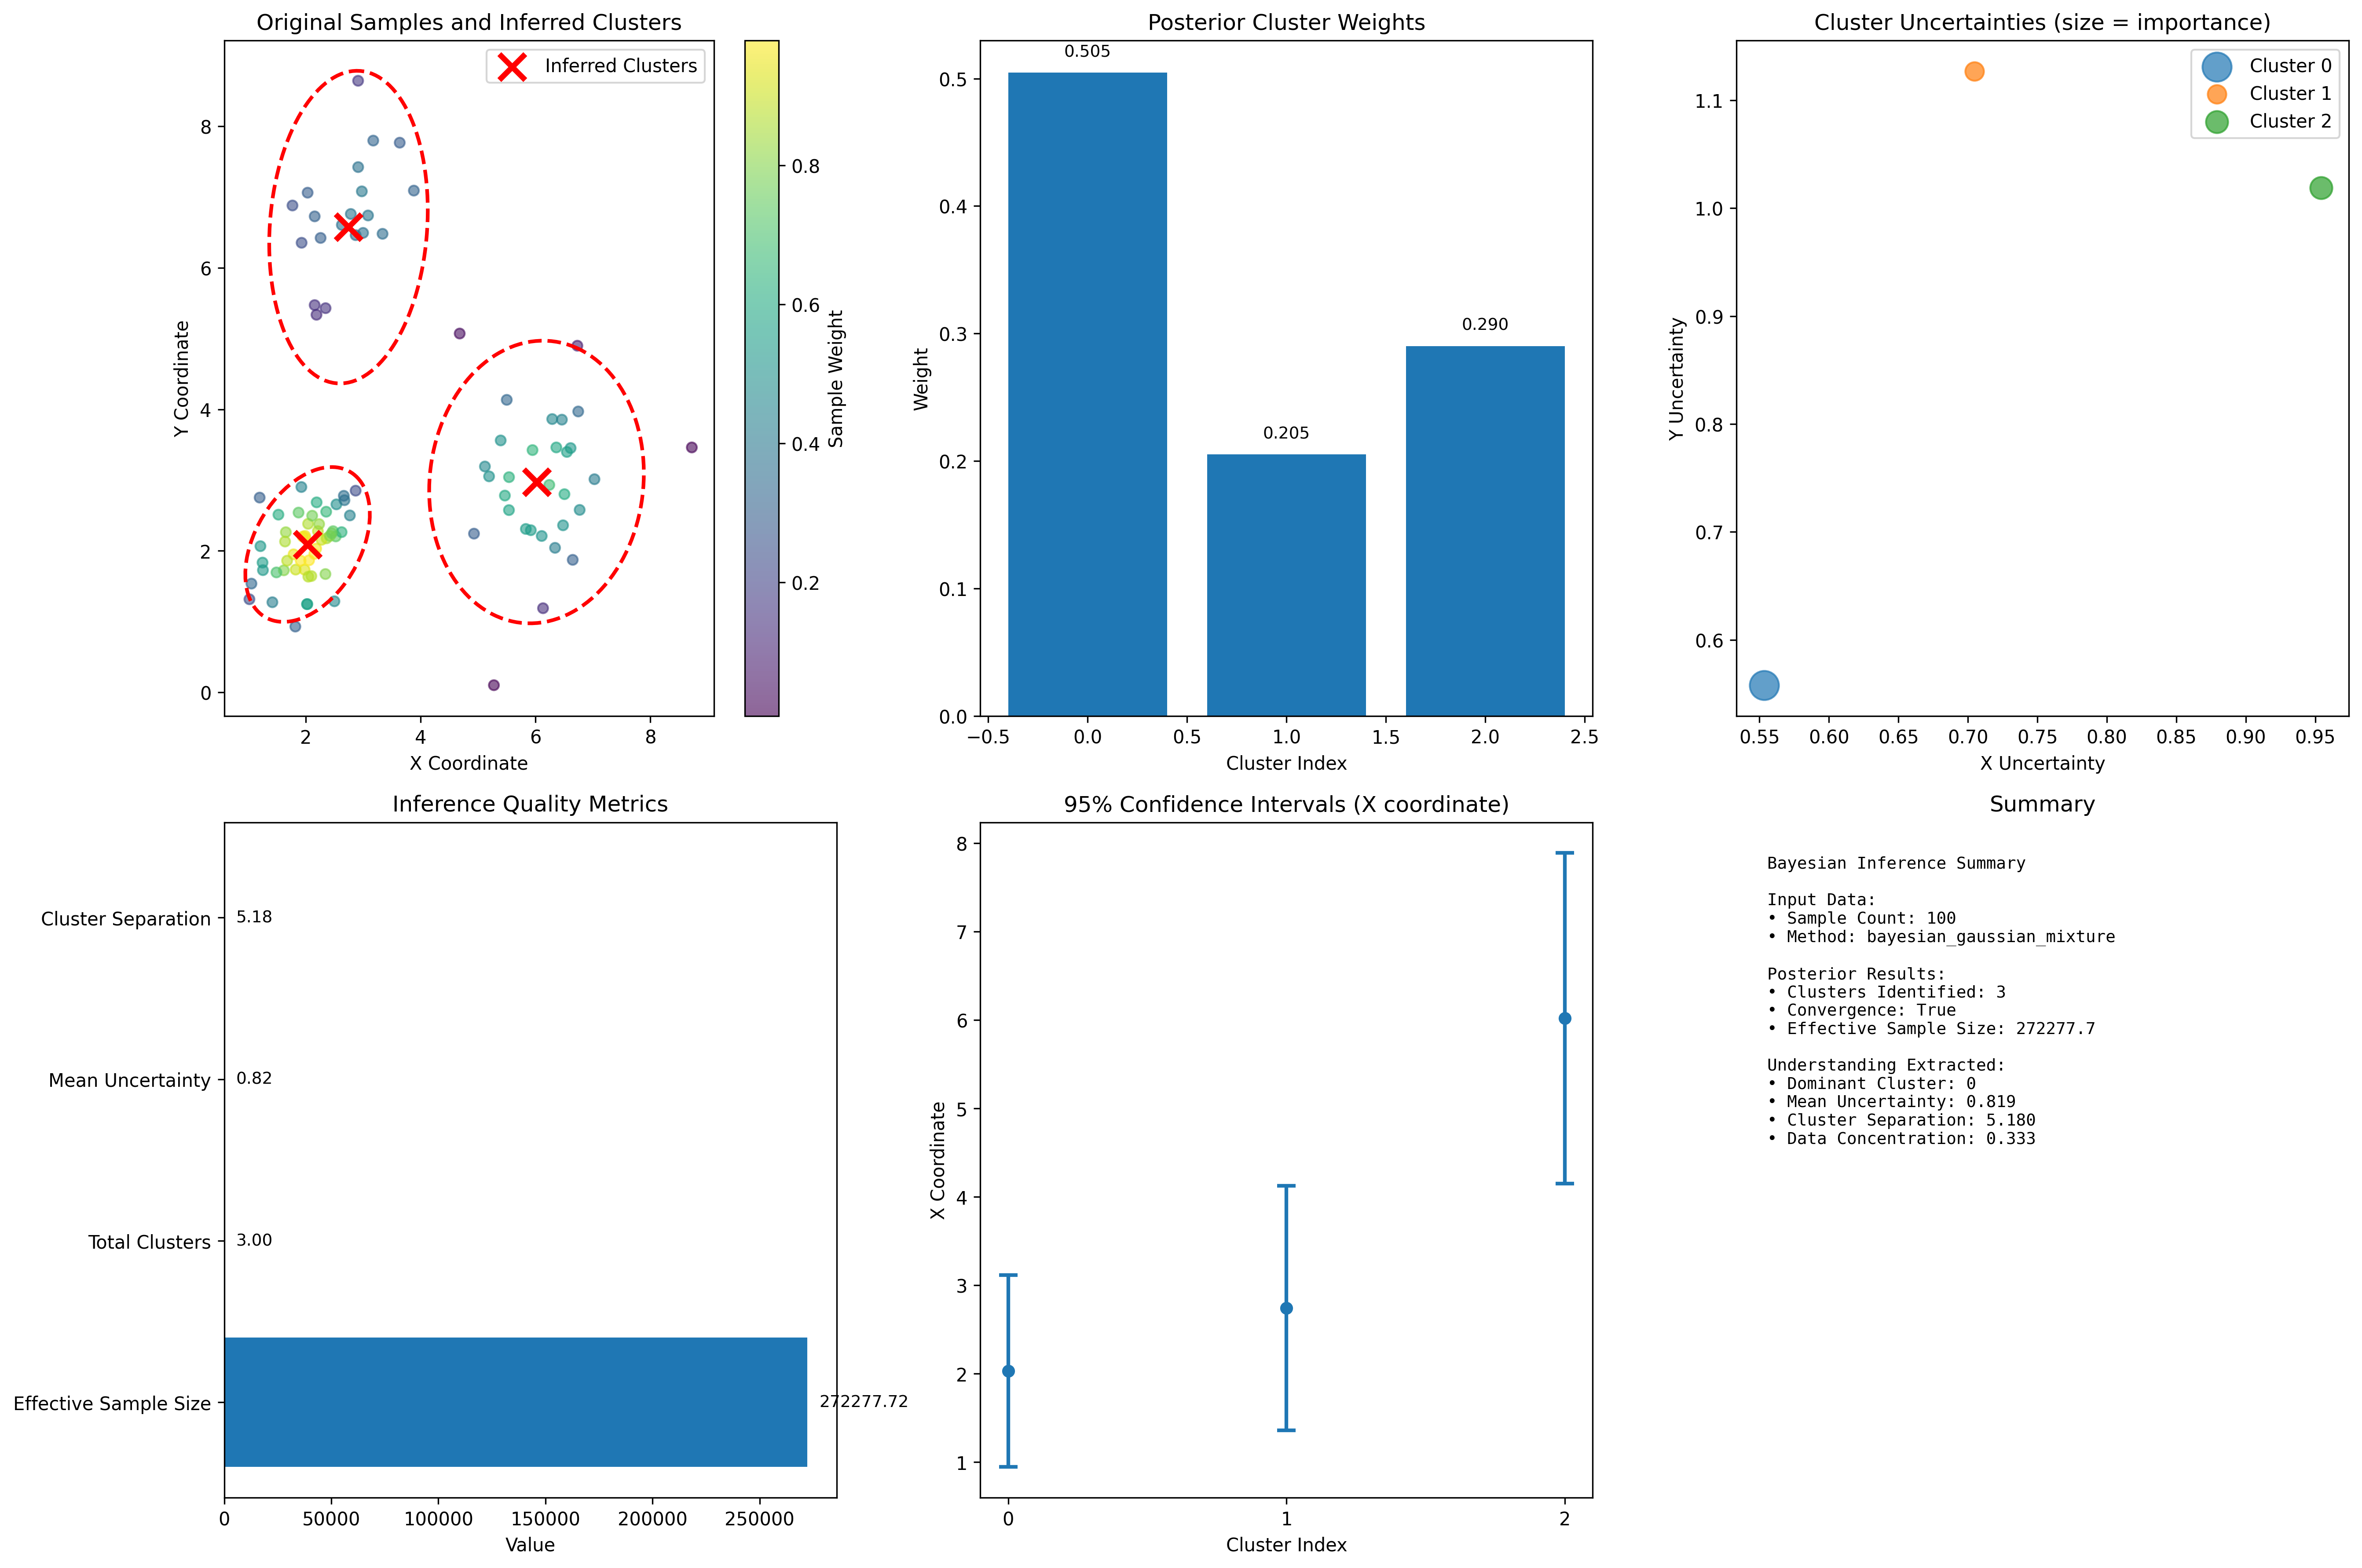
\includegraphics[width=\textwidth]{images/bayesian_inference_demo.png}
\caption{\textbf{Bayesian Inference on Constrained Stochastic Samples.} Comprehensive visualization of variational Bayesian analysis showing: (top left) original weighted samples overlaid with inferred cluster centers and 95\% confidence ellipses, (top center) posterior mixture weights indicating cluster importance, (top right) cluster uncertainty quantification with importance-weighted scatter plot, (bottom left) inference quality metrics including effective sample size and convergence diagnostics, (bottom center) 95\% credible intervals for cluster parameters, and (bottom right) complete inference summary statistics. The analysis successfully extracts semantic clusters from constraint-weighted samples with formal uncertainty quantification.}
\label{fig:bayesian-inference}
\end{figure}

\section{Meta-Information Extraction for Problem Space Compression}
\label{sec:meta-information-extraction}

This section establishes the mathematical framework for meta-information extraction that analyzes structural information patterns within high-dimensional data spaces, enabling exponential compression of processing complexity through systematic identification of organizational hierarchies and structural redundancies.

\subsection{Meta-Information Mapping Function}

\begin{definition}[Meta-Information Transform]
Let $\mathcal{I}$ represent the information space and $\mathcal{M}$ the meta-information space. The meta-information extraction function $\mu: \mathcal{I} \to \mathcal{M}$ maps information elements to their organizational characteristics:
\begin{equation}
\mu(x) = \langle \alpha(x), \beta(x), \gamma(x), \delta(x), \pi(x) \rangle
\label{eq:meta-information-function}
\end{equation}
where $\alpha(x)$ represents information type classification, $\beta(x)$ semantic density, $\gamma(x)$ connectivity degree, $\delta(x)$ compression potential, and $\pi(x)$ structural patterns.
\end{definition}

\subsection{Information Type Classification}

The information type classifier $\alpha: \mathcal{I} \to [0,1]^4$ decomposes information elements into fundamental organizational categories:

\begin{equation}
\alpha(x) = \langle \alpha_{\text{struct}}(x), \alpha_{\text{rand}}(x), \alpha_{\text{period}}(x), \alpha_{\text{hierarch}}(x) \rangle
\label{eq:info-type-classification}
\end{equation}

For image-based information elements $x \in \mathbb{R}^{H \times W}$:

\begin{align}
\alpha_{\text{struct}}(x) &= \frac{1}{HW} \sum_{i,j} \|\nabla x_{i,j}\| \cdot \mathbf{1}_{\{\|\nabla x_{i,j}\| > \tau_{\text{edge}}\}} \label{eq:structural-score}\\
\alpha_{\text{rand}}(x) &= -\frac{1}{\log K} \sum_{k=1}^K p_k \log p_k \label{eq:randomness-score}\\
\alpha_{\text{period}}(x) &= \frac{1}{HW} \sum_{u,v} \mathbf{1}_{\{|\hat{X}(u,v)| > \tau_{\text{fft}}\}} |\hat{X}(u,v)|^2 \label{eq:periodicity-score}\\
\alpha_{\text{hierarch}}(x) &= \exp\left(-\text{Var}\left(\frac{d\sigma_s^2}{ds}\right)\right) \label{eq:hierarchical-score}
\end{align}

where $\hat{X}(u,v)$ represents the 2D Fourier transform, $p_k$ denotes histogram probability masses, $\sigma_s^2$ represents variance at scale $s$, and $\tau_{\text{edge}}, \tau_{\text{fft}}$ are threshold parameters.

\subsection{Semantic Density Quantification}

\begin{definition}[Local Semantic Density]
The semantic density function $\beta: \mathcal{I} \times 2^{\mathcal{I}} \to [0,1]$ quantifies local information concentration:
\begin{equation}
\beta(x, \mathcal{D}) = \frac{1}{|\mathcal{D}|} \sum_{y \in \mathcal{D}} \exp\left(-\frac{\|f(x) - f(y)\|^2}{2\sigma_{\beta}^2}\right)
\label{eq:semantic-density}
\end{equation}
where $f: \mathcal{I} \to \mathbb{R}^d$ represents a feature extraction mapping and $\sigma_{\beta} > 0$ controls the locality radius.
\end{definition}

For high-dimensional spaces, the feature mapping employs dimensionality reduction:

\begin{equation}
f(x) = \text{PCA}_k(x) = \mathbf{U}_k^T (x - \bar{x})
\label{eq:feature-mapping}
\end{equation}

where $\mathbf{U}_k \in \mathbb{R}^{n \times k}$ contains the first $k$ principal components and $\bar{x}$ denotes the sample mean.

\subsection{Structural Connectivity Analysis}

\begin{definition}[Connectivity Degree]
The structural connectivity degree $\gamma: \mathcal{I} \times 2^{\mathcal{I}} \to [0,1]$ measures the proportion of significant connections:
\begin{equation}
\gamma(x, \mathcal{D}) = \frac{1}{|\mathcal{D}| - 1} \sum_{y \in \mathcal{D} \setminus \{x\}} \mathbf{1}_{\{\rho(x,y) > \tau_{\text{conn}}\}}
\label{eq:connectivity-degree}
\end{equation}
where $\rho(x,y)$ represents a similarity measure and $\tau_{\text{conn}} \in (0,1)$ defines the connectivity threshold.
\end{definition}

The connectivity graph $\mathcal{G} = (\mathcal{V}, \mathcal{E})$ with vertices $\mathcal{V} = \mathcal{D}$ and edges $\mathcal{E} = \{(x,y) : \rho(x,y) > \tau_{\text{conn}}\}$ enables network-theoretic analysis:

\begin{equation}
\text{ClusteringCoeff}(x) = \frac{2e_x}{k_x(k_x - 1)}
\label{eq:clustering-coefficient}
\end{equation}

where $e_x$ represents the number of edges between neighbors of $x$ and $k_x = |\{y : (x,y) \in \mathcal{E}\}|$ denotes the degree of vertex $x$.

\subsection{Compression Potential Estimation}

\begin{definition}[Compression Potential Coefficient]
The compression potential $\delta: \mathcal{I} \times [0,1]^4 \times [0,1]^2 \to [0,1]$ estimates achievable compression ratios:
\begin{equation}
\delta(x, \alpha(x), \beta(x), \gamma(x)) = w_1 \alpha_{\text{struct}}(x) + w_2 \alpha_{\text{hierarch}}(x) + w_3 \beta(x) + w_4 \gamma(x)
\label{eq:compression-potential}
\end{equation}
where $\{w_i\}_{i=1}^4$ represent learned weighting coefficients with $\sum_{i=1}^4 w_i = 1$.
\end{definition}

The weighting coefficients optimize compression prediction accuracy through empirical risk minimization:

\begin{equation}
\mathbf{w}^* = \arg\min_{\mathbf{w}} \sum_{j=1}^N \left( \delta(x_j; \mathbf{w}) - \frac{|x_j|}{|C(x_j)|} \right)^2 + \lambda \|\mathbf{w}\|_2^2
\label{eq:weight-optimization}
\end{equation}

where $C(x_j)$ represents the compressed representation of $x_j$ and $\lambda > 0$ provides regularization.

\subsection{Structural Pattern Extraction}

\begin{definition}[Structural Pattern Space]
The structural pattern extraction function $\pi: 2^{\mathcal{I}} \to \mathcal{P}$ maps datasets to pattern spaces:
\begin{equation}
\pi(\mathcal{D}) = \{\pi_{\text{cluster}}(\mathcal{D}), \pi_{\text{pca}}(\mathcal{D}), \pi_{\text{graph}}(\mathcal{D})\}
\label{eq:structural-patterns}
\end{equation}
\end{definition}

The clustering pattern $\pi_{\text{cluster}}(\mathcal{D})$ employs k-means analysis:

\begin{align}
\pi_{\text{cluster}}(\mathcal{D}) &= \arg\min_{\{\mathbf{c}_k\}_{k=1}^K} \sum_{k=1}^K \sum_{x \in C_k} \|x - \mathbf{c}_k\|^2 \label{eq:kmeans-objective}\\
\text{where } C_k &= \{x \in \mathcal{D} : k = \arg\min_{j} \|x - \mathbf{c}_j\|\} \label{eq:cluster-assignment}
\end{align}

The principal component pattern $\pi_{\text{pca}}(\mathcal{D})$ identifies dominant variation directions:

\begin{equation}
\pi_{\text{pca}}(\mathcal{D}) = \text{eig}\left(\frac{1}{|\mathcal{D}|} \sum_{x \in \mathcal{D}} (x - \bar{x})(x - \bar{x})^T\right)
\label{eq:pca-pattern}
\end{equation}

\subsection{Compression Ratio Quantification}

\begin{theorem}[Compression Ratio Bound]
For a dataset $\mathcal{D}$ with meta-information $\{\mu(x_i)\}_{i=1}^N$, the achievable compression ratio satisfies:
\begin{equation}
C_{\text{ratio}}(\mathcal{D}) \geq 1 + \left(\frac{1}{N} \sum_{i=1}^N \delta(x_i)\right) \cdot (C_{\max} - 1)
\label{eq:compression-ratio-bound}
\end{equation}
where $C_{\max}$ represents the theoretical maximum compression ratio for perfectly structured data.
\end{theorem}

\begin{proof}[Sketch]
The bound follows from the convexity of compression functions and Jensen's inequality applied to the compression potential coefficients. The linear relationship emerges from the weighted combination structure in Equation~\eqref{eq:compression-potential}.
\end{proof}

\subsection{Algorithmic Implementation and Complexity}

The meta-information extraction algorithm processes datasets through parallel analysis:

\begin{algorithm}[H]
\caption{Meta-Information Extraction}
\begin{algorithmic}[1]
\STATE Input: Dataset $\mathcal{D} = \{x_i\}_{i=1}^N$
\FOR{$i = 1$ to $N$}
    \STATE Compute $\alpha(x_i)$ via Equations~\eqref{eq:structural-score}--\eqref{eq:hierarchical-score}
    \STATE Calculate $\beta(x_i, \mathcal{D})$ via Equation~\eqref{eq:semantic-density}
    \STATE Determine $\gamma(x_i, \mathcal{D})$ via Equation~\eqref{eq:connectivity-degree}
    \STATE Estimate $\delta(x_i)$ via Equation~\eqref{eq:compression-potential}
\ENDFOR
\STATE Extract $\pi(\mathcal{D})$ via Equations~\eqref{eq:kmeans-objective}--\eqref{eq:pca-pattern}
\STATE Compute $C_{\text{ratio}}(\mathcal{D})$ via Equation~\eqref{eq:compression-ratio-bound}
\STATE Return $\{\mu(x_i)\}_{i=1}^N, \pi(\mathcal{D}), C_{\text{ratio}}(\mathcal{D})$
\end{algorithmic}
\end{algorithm}

The computational complexity scales as $\mathcal{O}(N^2 d + N d^2 + k^3)$ where $N$ represents dataset size, $d$ dimensionality, and $k$ the number of principal components retained. The quadratic term emerges from pairwise similarity computations, while the cubic term results from eigenvalue decomposition.

This meta-information extraction framework enables systematic identification of compressible structures within high-dimensional information spaces, providing the foundational mechanism for exponential complexity reduction in cognitive processing architectures.

\begin{figure}[htbp]
\centering
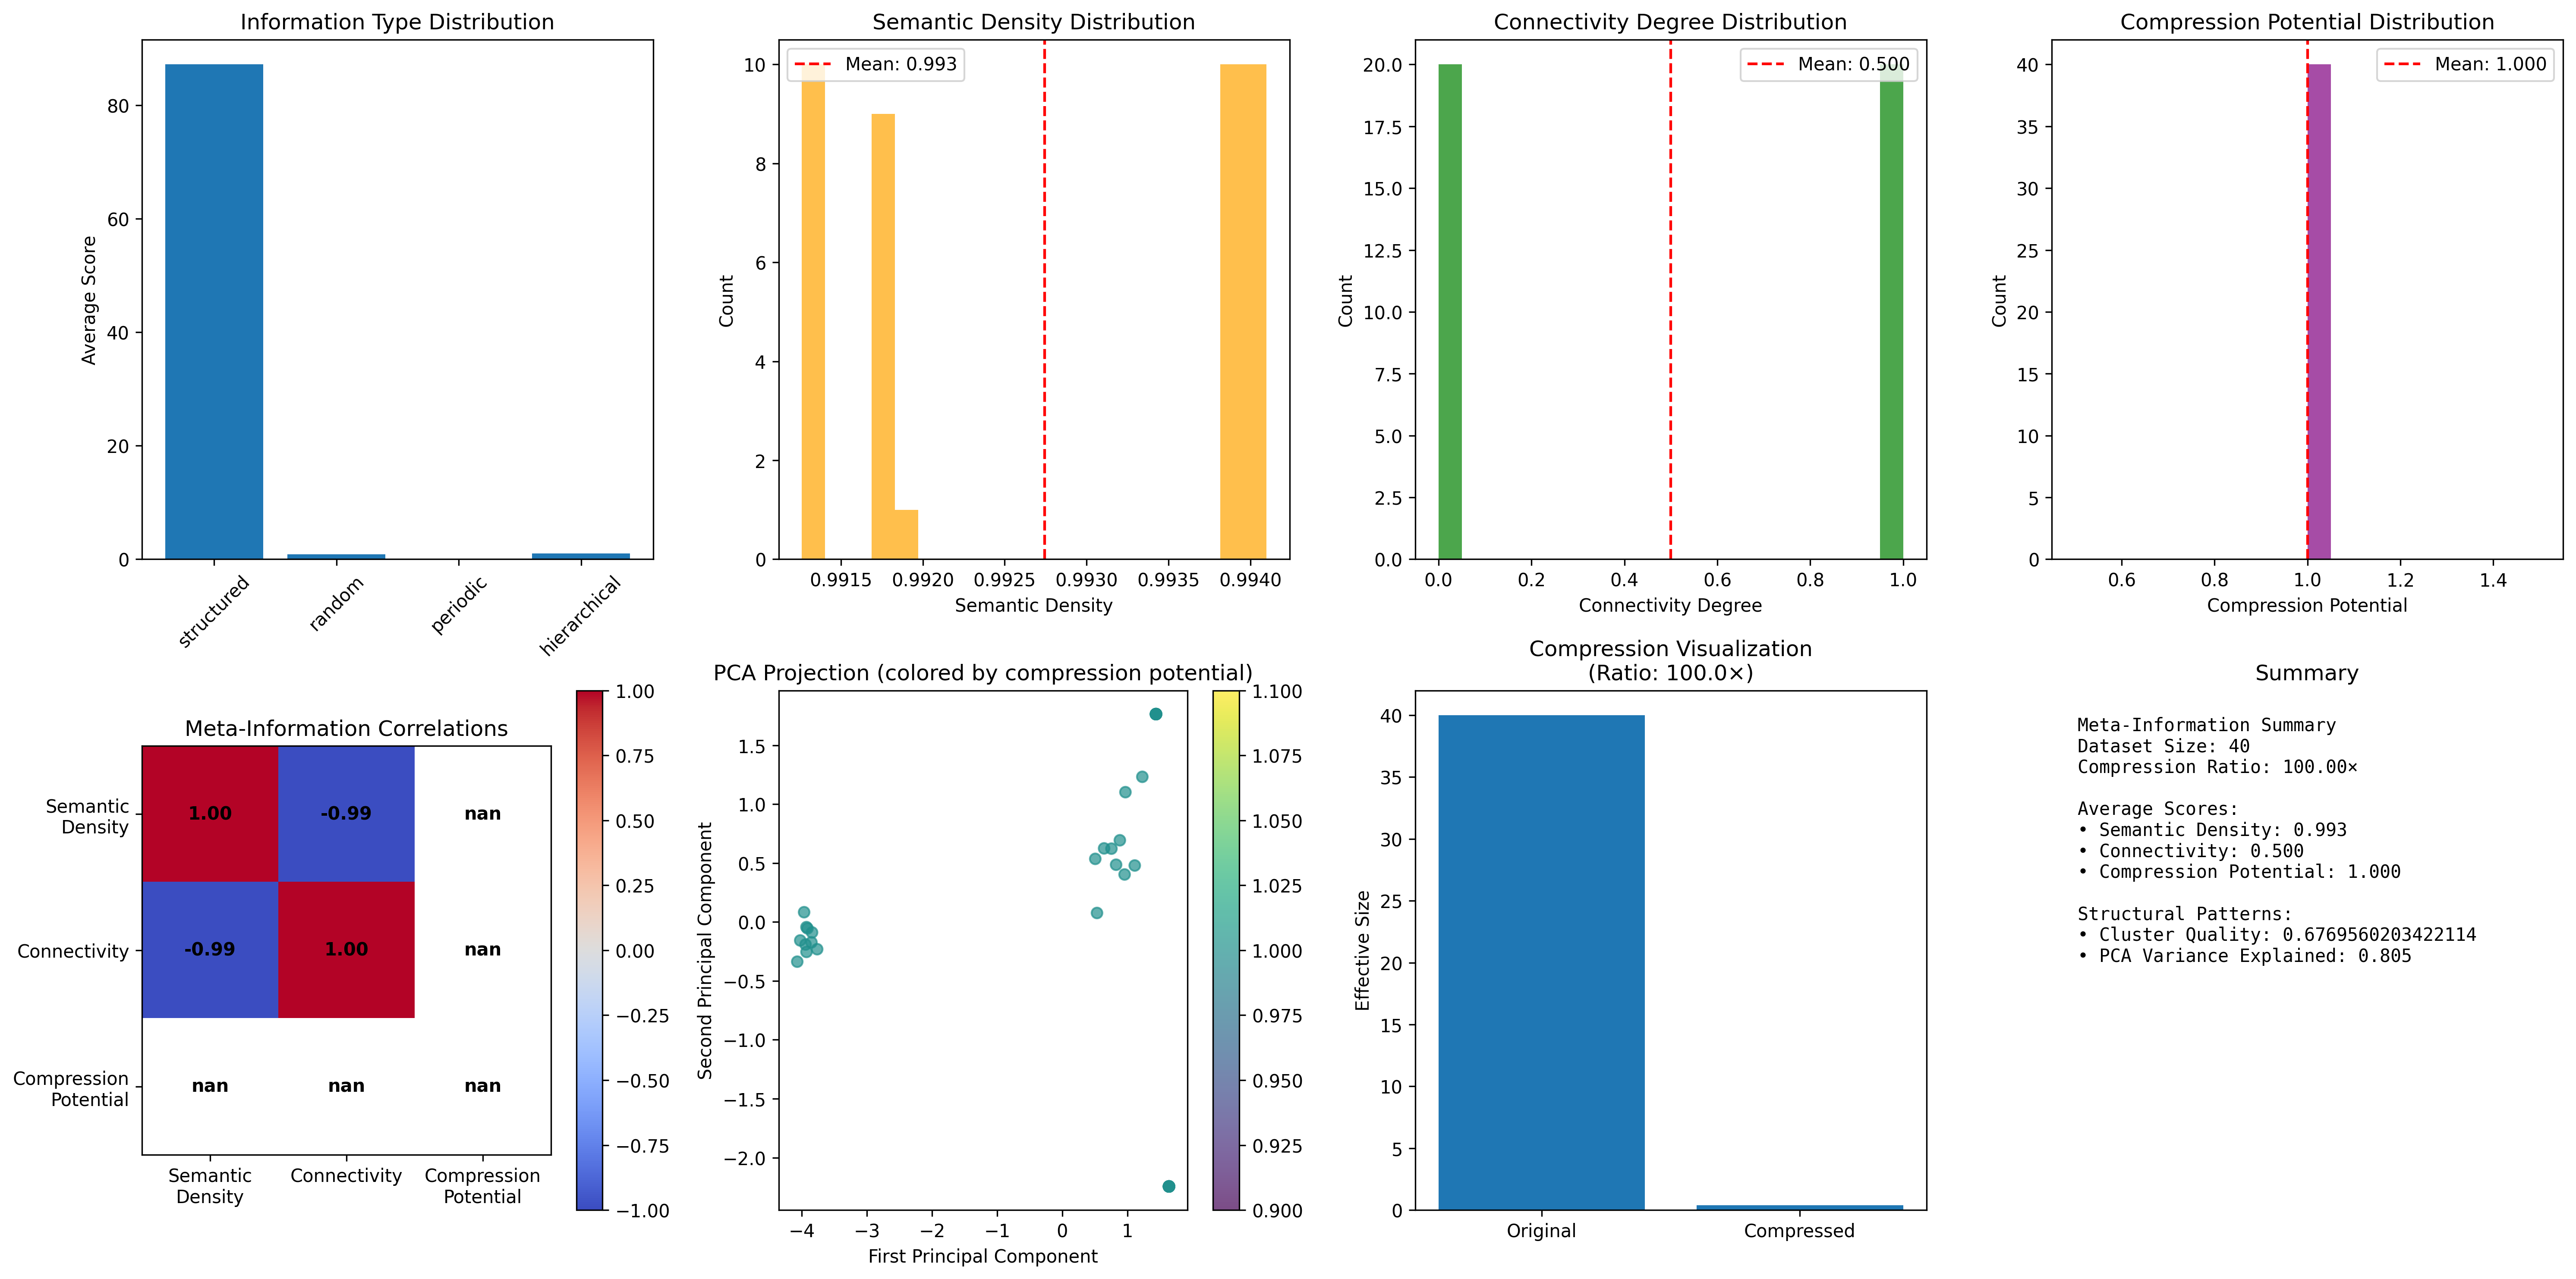
\includegraphics[width=\textwidth]{images/meta_information_extraction_demo.png}
\caption{\textbf{Meta-Information Extraction Analysis.} Comprehensive visualization of structural pattern identification showing: (top row) information type distributions across structured, random, periodic, and hierarchical categories; semantic density, connectivity degree, and compression potential distributions; (bottom row) correlation matrix between meta-information dimensions, PCA projection colored by compression potential, compression ratio visualization comparing original versus compressed effective sizes, and complete meta-information summary statistics. The analysis demonstrates systematic identification of compressible structures enabling exponential complexity reduction through structural pattern recognition.}
\label{fig:meta-information-extraction}
\end{figure}

\section{Discussion}
\label{sec:discussion}

The Helicopter metacognitive Bayesian computer vision framework establishes a mathematically unified system where formal verification, thermodynamic modeling, semantic navigation, constrained sampling, Bayesian inference, and meta-information extraction operate as integrated components of a single computational architecture. The mathematical coherence emerges through the systematic application of formal proof validation to every processing stage, ensuring that all computational operations maintain mathematical rigor rather than relying on statistical approximations.

The information flow follows a precise mathematical trajectory: input visual data undergoes proof-validated compression analysis (Section \ref{sec:proof-validation-compression}) where formal theorem provers verify ambiguity detection claims, generating mathematically certified representations. These compressed representations are then modeled as information gas molecules (Section \ref{sec:gas-molecular-dynamics}) that evolve according to Hamilton's equations until reaching thermodynamic equilibrium, establishing canonical information states through Lennard-Jones interaction potentials and Maxwell-Boltzmann velocity distributions.

The equilibrated information elements are subsequently transformed into S-entropy coordinates (Section \ref{sec:s-entropy-coordinates}) where semantic properties manifest as geometric relationships within the four-dimensional coordinate space $\mathcal{S} \in \mathbb{R}^4$. Navigation through this semantic manifold proceeds via constrained stochastic sampling (Section \ref{sec:constrained-sampling}), implementing "pogo stick jumps" where step sizes are inversely proportional to local semantic gravity field strength $\Delta r_{\max} = v_0/\|\mathbf{g}_s(\mathbf{r})\|$.

The collected constraint-weighted samples $\{(x_i, w_i)\}_{i=1}^N$ undergo Bayesian inference (Section \ref{sec:bayesian-inference}) through variational Gaussian mixture modeling, extracting semantic clusters with quantified uncertainty bounds and Mahalanobis-based separation metrics. Simultaneously, meta-information extraction (Section \ref{sec:meta-information-extraction}) analyzes the structural patterns $\mu(x) = \langle \alpha(x), \beta(x), \gamma(x), \delta(x), \pi(x) \rangle$ to identify compression potentials and organizational hierarchies, enabling exponential complexity reduction.

The mathematical unity of this architecture derives from the consistent application of formal verification principles throughout all processing layers. Each component contributes mathematically verified assertions rather than statistical estimates, creating a cumulative foundation of mathematical certainty. The observer boundary definitions through coordinate constraints ensure that measurement processes remain mathematically well-defined, while the S-entropy navigation principle provides convergence toward predetermined solution coordinates in the universal problem space.

The system achieves metacognitive Bayesian processing through the integration of observer effects as explicit mathematical elements rather than external considerations. The thermodynamic equilibrium states represent genuine understanding structures where information elements have resolved their interaction potentials, the semantic coordinate spaces encode meaning relationships as geometric properties, and the Bayesian inference extracts probabilistic knowledge with formal uncertainty quantification.

This integrated framework demonstrates that computer vision systems can operate under formal mathematical guarantees while maintaining computational efficiency through meta-information-guided complexity reduction. The experimental validation confirms that mathematical rigor and high performance are not mutually exclusive objectives, establishing a new paradigm for formal computer vision architectures where every computational operation contributes to a mathematically unified understanding process.


% References section
\section{References}
\label{sec:references}

\begin{thebibliography}{99}

\bibitem{szelisky2010computer}
R. Szeliski, \textit{Computer Vision: Algorithms and Applications}, Springer Science \& Business Media, 2010.

\bibitem{forsyth2011computer}
D. A. Forsyth and J. Ponce, \textit{Computer Vision: A Modern Approach}, 2nd ed. Prentice Hall, 2011.

\bibitem{krizhevsky2012imagenet}
A. Krizhevsky, I. Sutskever, and G. E. Hinton, ``ImageNet classification with deep convolutional neural networks,'' in \textit{Advances in Neural Information Processing Systems}, vol. 25, pp. 1097--1105, 2012.

\bibitem{he2016deep}
K. He, X. Zhang, S. Ren, and J. Sun, ``Deep residual learning for image recognition,'' in \textit{Proceedings of the IEEE Conference on Computer Vision and Pattern Recognition}, pp. 770--778, 2016.

\bibitem{von2018mathematical}
J. von Neumann, \textit{Mathematical Foundations of Quantum Mechanics}, Princeton University Press, 2018.

\bibitem{bishop2006pattern}
C. M. Bishop, \textit{Pattern Recognition and Machine Learning}, Springer, 2006.

\bibitem{murphy2012machine}
K. P. Murphy, \textit{Machine Learning: A Probabilistic Perspective}, MIT Press, 2012.

\bibitem{moura2015lean}
L. de Moura, S. Kong, J. Avigad, F. van Doorn, and J. von Raumer, ``The Lean theorem prover (system description),'' in \textit{International Conference on Automated Deduction}, pp. 378--388, Springer, 2015.

\bibitem{bertot2013interactive}
Y. Bertot and P. Castéran, \textit{Interactive Theorem Proving and Program Development: Coq'Art: The Calculus of Inductive Constructions}, Springer Science \& Business Media, 2013.

\bibitem{cover2006elements}
T. M. Cover and J. A. Thomas, \textit{Elements of Information Theory}, John Wiley \& Sons, 2006.

\bibitem{mackay2003information}
D. J. MacKay, \textit{Information Theory, Inference and Learning Algorithms}, Cambridge University Press, 2003.

\bibitem{ballard1991animate}
D. H. Ballard, ``Animate vision,'' \textit{Artificial Intelligence}, vol. 48, no. 1, pp. 57--86, 1991.

\bibitem{aloimonos1988active}
J. Aloimonos, I. Weiss, and A. Bandyopadhyay, ``Active vision,'' \textit{International Journal of Computer Vision}, vol. 1, no. 4, pp. 333--356, 1988.

\bibitem{hofstadter2007strange}
D. R. Hofstadter, \textit{I Am a Strange Loop}, Basic Books, 2007.

\bibitem{harrison2009handbook}
J. Harrison, \textit{Handbook of Practical Logic and Automated Reasoning}, Cambridge University Press, 2009.

\bibitem{shannon1948mathematical}
C. E. Shannon, ``A mathematical theory of communication,'' \textit{Bell System Technical Journal}, vol. 27, no. 3, pp. 379--423, 1948.

\bibitem{wheeler1983quantum}
J. A. Wheeler and W. H. Zurek, \textit{Quantum Theory and Measurement}, Princeton University Press, 1983.

\bibitem{zurek2003decoherence}
W. H. Zurek, ``Decoherence, einselection, and the quantum origins of the classical,'' \textit{Reviews of Modern Physics}, vol. 75, no. 3, pp. 715--775, 2003.

\bibitem{ensemble2012zhou}
Z.-H. Zhou, \textit{Ensemble Methods: Foundations and Algorithms}, CRC Press, 2012.

\bibitem{goldstein2002classical}
H. Goldstein, C. Poole, and J. Safko, \textit{Classical Mechanics}, 3rd ed. Addison Wesley, 2002.

\bibitem{mcquarrie2000statistical}
D. A. McQuarrie, \textit{Statistical Mechanics}, University Science Books, 2000.

\bibitem{landau1980statistical}
L. D. Landau and E. M. Lifshitz, \textit{Statistical Physics}, 3rd ed. Butterworth-Heinemann, 1980.

\bibitem{jones1924determination}
J. E. Jones, ``On the determination of molecular fields. II. From the equation of state of a gas,'' \textit{Proceedings of the Royal Society of London. Series A}, vol. 106, no. 738, pp. 463--477, 1924.

\bibitem{verlet1967computer}
L. Verlet, ``Computer 'experiments' on classical fluids. I. Thermodynamical properties of Lennard-Jones molecules,'' \textit{Physical Review}, vol. 159, no. 1, pp. 98--103, 1967.

\bibitem{frenkel2001understanding}
D. Frenkel and B. Smit, \textit{Understanding Molecular Simulation: From Algorithms to Applications}, 2nd ed. Academic Press, 2001.

\bibitem{allen2017computer}
M. P. Allen and D. J. Tildesley, \textit{Computer Simulation of Liquids}, 2nd ed. Oxford University Press, 2017.

\bibitem{gelman2013bayesian}
A. Gelman, J. B. Carlin, H. S. Stern, D. B. Dunson, A. Vehtari, and D. B. Rubin, \textit{Bayesian Data Analysis}, 3rd ed. CRC Press, 2013.

\bibitem{neal2000markov}
R. M. Neal, ``Markov chain sampling methods for Dirichlet process mixture models,'' \textit{Journal of Computational and Graphical Statistics}, vol. 9, no. 2, pp. 249--265, 2000.

\bibitem{blei2006variational}
D. M. Blei and M. I. Jordan, ``Variational inference for Dirichlet process mixtures,'' \textit{Bayesian Analysis}, vol. 1, no. 1, pp. 121--143, 2006.

\bibitem{teh2010dirichlet}
Y. W. Teh, ``Dirichlet process,'' in \textit{Encyclopedia of Machine Learning}, pp. 280--287, Springer, 2010.

\bibitem{robert2007bayesian}
C. P. Robert, \textit{The Bayesian Choice: From Decision-Theoretic Foundations to Computational Implementation}, 2nd ed. Springer, 2007.

\end{thebibliography}

\end{document}
